\documentclass[12pt, a4paper]{report}
\usepackage{graphicx}
\usepackage{colortbl}
\usepackage[brazilian]{babel}
\usepackage[utf8x]{inputenc}
\usepackage{setspace}
\usepackage{hyperref}
\usepackage[small,bf]{caption}
\usepackage{amsmath, amssymb, pxfonts}
\usepackage{textcomp}
\usepackage{nomencl}
\makenomenclature
\usepackage{longtable}
\usepackage{tikz}
\usepackage{pgfplots}
\usepackage{mathrsfs}
\everymath{\displaystyle}
\usepackage[alf]{abntex2cite}
\usepackage{url}
\usepackage{emptypage}
\usepackage{fancyhdr}
\usepackage{lastpage}
\usepackage{nopageno}
\usepackage{indentfirst}
\usepackage{parskip}
\usepackage{titlesec}
\usepackage{listings}
\usepackage{subfig}
\usepackage{verbatim}
\usepackage{multirow}
%\usepackage[makeindex,split]{splitidx}

%%%%%%%%%%%%%%%%%%%%%%%%%%%%%%%%%%%%%%%%%%%%%%%%%%%%%%%%%%%%%%%%%%%%
%%%
%%% Macros 
%%% Curso de Especialização em Sistemas Eletrônicos para Controle
%%% Faculdade SENAI Anchieta - São Paulo - SP
%%% José William Rodrigues Pereira 
%%% Outubro / 2015
%%%
%%%%%%%%%%%%%%%%%%%%%%%%%%%%%%%%%%%%%%%%%%%%%%%%%%%%%%%%%%%%%%%%%%%%

%%%------------------------------------ Dados
\def\autor#1{\gdef\autor{#1}}
\def\nome#1{\gdef\nome{#1}}
\def\ultimonome#1{\gdef\ultimonome{#1}}
\def\titulo#1{\gdef\titulo{#1}}
\def\subtitulo#1{\gdef\subtitulo{#1}}
\def\curso#1{\gdef\curso{#1}}
\def\instituicao#1{\gdef\instituicao{#1}}
\def\sigla#1{\gdef\sigla{#1}}
\def\unidadeacademica#1{\gdef\unidadeacademica{#1}}
\def\grau#1{\gdef\grau{#1}}
\def\tipodotrabalho#1{\gdef\tipodotrabalho{#1}}
\def\orientador#1{\gdef\orientador{#1}}
\def\torientador#1{\gdef\torientador{#1}}
\def\coorientador#1{\gdef\coorientador{#1}}
\def\tcoorientador#1{\gdef\tcoorientador{#1}}
\def\cidade#1{\gdef\cidade{#1}}
\def\ano#1{\gdef\ano{#1}}
\def\npaginas#1{\gdef\npaginas{#1}}
\def\CDU#1{\gdef\CDU{#1}}
\def\areas#1{\gdef\areas{#1}}
\def\examinadorum#1{\gdef\examinadorum{#1}}
\def\texaminadorum#1{\gdef\texaminadorum{#1}}
\def\examinadordois#1{\gdef\examinadordois{#1}}
\def\texaminadordois#1{\gdef\texaminadordois{#1}}
\def\data#1{\gdef\data{#1}}
\def\palavraschave#1{\gdef\palavraschave{#1}}
\def\keywords#1{\gdef\keywords{#1}}

%%%%------------------------------------ Configuração das Páginas
\newcommand{\configuramargens} %%% Define margens
{
  \usepackage[width=210.00mm, height=297.00mm, 
			  left=3.00cm,    right=2.00cm, 
			  top=3.00cm,     bottom=2.00cm] {geometry}
}

%%%------------------------------------ Fonte
%\renewcommand{\familydefault}{\sfdefault} % sans font
\renewcommand{\familydefault}{\rmdefault}  % roman font


%%%------------------------------------ Formatação de Capitulo
\titleformat{\chapter}
  {\Large\bfseries}
  {}
  {0pt}
  {\huge}

%%%------------------------------------ Capa
\newcommand{\capa}
{
  \begin{titlepage}
    \thispagestyle{empty}
    \begin{center}
      \textsc{\instituicao} 		\\[5.0cm]
%      \textsc{\unidadeacademica}	\\[0.0cm]
%      \textsc{Curso de \curso}		\\[4.0cm]
      \textsc{\autor}			\\[5.0cm]
      \textsc{\titulo}			\\[0.0cm]
      \textsc{\subtitulo}               \\[0.4cm]
      \vfill
      \textsc{\cidade}			\\[0.0cm]
      \textsc{\ano}			\\[0.0cm]
    \end{center}
  \end{titlepage}
}
%%%------------------------------------ Natureza
\newcommand{\natureza}
{
  \begin{flushright}
    \thispagestyle{empty}
    \begin{minipage}{0.54\textwidth}
    {
      \tipodotrabalho apresentada ao \instituicao 
      como requisito para 
      obtenção do grau de \grau em \curso
    } 				\\[0.4cm]
    Orientador:   \torientador    \orientador \\
%    Coorientador: \tcoorientador  \coorientador
    \end{minipage}
  \end{flushright}
}
%%%------------------------------------ Folha de Rosto
\newcommand{\folhaderosto}
{
  \begin{titlepage}
    \begin{center}
      \textsc{ }		\\[5.0cm]
      \textsc{\autor}		\\[5.0cm]
      \textsc{\titulo}		\\[0.0cm]
      \textsc{\subtitulo}       \\[4.0cm]
      \natureza
      \vfill
      \textsc{\cidade}		\\[0.0cm]
      \textsc{\ano}		\\[0.0cm]
    \end{center}
  \end{titlepage}
}
%%%------------------------------------ Ficha Catalográfica
\newcommand{\fichacatalografica}
{
  \begin{titlepage}
    \vfil\null
    \vfill
    \fbox
    {
      \begin{tabular}{p{14.0cm}}
        P492c \ultimonome, \nome \\
	\hspace{1cm} \begin{minipage}{0.8\textwidth}
             \hspace{1cm} \titulo \subtitulo\ / \nome\ \ultimonome\ , - - \cidade , \ano .\\
            \npaginas f. : il   					\\
									\\
	    \hspace{1cm} Orientador: \orientador . 			\\
	    \hspace{1cm} \grau (\curso ) - - 				\\
	    \hspace{1cm} \instituicao , \ano .				\\
									\\
            \areas . I. Leão, Tarcisio Fernandes. II. Título. 		\\
									\\
	    \begin{flushright}
            \hfill CDD \CDU
	    \end{flushright}
        \end{minipage}
      \end{tabular} 
    }  
 \end{titlepage}
}
%%%------------------------------------ Folha de Aprovação
\newcommand{\folhadeaprovacao}
{
  \begin{titlepage}
    \thispagestyle{empty}
    \begin{center}
      \textsc{\autor}
      \vfill
      \textsc{ \titulo } \\
      \textsc{ \subtitulo }
      \vfill
    \end{center}
    \natureza
    \vfill
    \centering Aprovado pela banca examinadora em \data \\
    \vfill
    \begin{center}
      {\large\bfseries BANCA EXAMINADORA }\\
      \vfill
      \rule{9.0cm}{0.1mm} \\
      {\torientador \orientador  }\\
      {Orientador } \\
 %     \vfill
 %     \rule{9.0cm}{0.1mm} \\
 %     {\tcoorientador \coorientador} \\
 %     {Coorientador} \\
      \vfill
      \rule{9.0cm}{0.1mm} \\
      {\texaminadorum \examinadorum }\\
      \vfill
      \rule{9.0cm}{0.1mm} \\
      {\texaminadordois \examinadordois}
    \end{center}
  \end{titlepage}
}
%%%------------------------------------ Dedicatória
\newcommand{\dedicatoria}[1]
{
  \begin{titlepage} 
    \thispagestyle{empty}
    \titlepage
    \begin{center}%
        \huge \textbf{Dedicatória}
    \end{center}%
    \null
    \hspace{1cm} #1
    \endtitlepage
  \end{titlepage}

%  \begin{titlepage}
%  \thispagestyle{empty}
%  \hspace{1cm}
%  \vfill
%  \begin{flushright}
%    \begin{minipage}{0.6\textwidth}
%    \textrm
%    {
%      \textit
%      {
%	#1
%      }
%    }    
%    \end{minipage}
%  \end{flushright}
%  \end{titlepage}
}

%%%------------------------------------ Agradecimentos
\newcommand{\agradecimentos}[1]
{
  \begin{titlepage} 
    \thispagestyle{empty}
    \titlepage
    \begin{center}%
        \huge \textbf{Agradecimentos}
    \end{center}%
    \null
    \hspace{1cm} #1
    \endtitlepage
  \end{titlepage}
}

%%%------------------------------------ Epígrafe
\newcommand{\epigrafe}[1]
{
  \begin{titlepage}
    \thispagestyle{empty} 
    \hspace{1cm}
    \vfill
    \begin{flushright}
      \begin{minipage}{0.6\textwidth}
      \textrm
      {
        \textit
        {
	    #1
        }
      }    
      \end{minipage}
    \end{flushright}
  \end{titlepage}
}

%%%------------------------------------ Resumo
\newcommand{\resumo}[1]
{
  \begin{titlepage} 
    \titlepage  
    \thispagestyle{empty}
    \begin{center}%
        \huge \textbf{Resumo}
    \end{center}%
    \null
    #1

    \textbf{\\PALAVRAS-CHAVE:} \palavraschave
    \endtitlepage
  \end{titlepage}
}
%-------------------------------------- Abstract
\newcommand{\resumolinguaestrangeira}[1]
{
  \begin{titlepage} 
    \titlepage
    \thispagestyle{empty}  
    \begin{center}%
        \huge \textbf{Abstract}
    \end{center}%
    \null  
    \hspace{1cm} 
    #1

    \textbf{\\KEYWORDS:} \keywords
    \endtitlepage
  \end{titlepage}
}
%-------------------------------------- Sumário
\newcommand{\sumario}
{
    \tableofcontents
    \thispagestyle{empty}
}
%-------------------------------------- Lista de figuras
\newcommand{\listadefiguras}
{
  \listoffigures
  \thispagestyle{empty}
}
%-------------------------------------- Lista de tabelas
\newcommand{\listadetabelas}
{
  \listoftables
  \thispagestyle{empty}
}

%-------------------------------------- Lista de abreviaturas e siglas
\newcommand{\abreviatura}[2]
{
  \nomenclature{#1}{#2}
  #1
}
\newcommand{\listadeabreviaturasesiglas}
{
  \renewcommand{\nomname}{Lista de abreviaturas e siglas}
  \printnomenclature[5em]
  \thispagestyle{empty}	
}
%%%------------------------------------ Citação
\newcommand{\citacao}[1]
{
  \begin{flushright}
    \begin{minipage}{12cm}
      \footnotesize #1
    \end{minipage}
    \vspace{12pt}
  \end{flushright}
}

%--------------------------------------
%--------------------------------------


%--------------------------------------
%-------------- Estilo do Codigo Fonte
\definecolor{verde}{rgb}{0.25,0.5,0.35}
\definecolor{jpurple}{rgb}{0.5,0,0.36}

\lstset{
  language=C,
  basicstyle=\ttfamily\small,
  keywordstyle=\color{blue},
  stringstyle=\color{verde},
  commentstyle=\color{red},
  extendedchars=true,
  showspaces=false,
  showstringspaces=false,
  numbers=left,
  numberstyle=\small,
  breaklines=true,
  backgroundcolor=\color{green!10},
  breakautoindent=true,
  captionpos=b,
  xleftmargin=0pt,
}

%--------------------------------------:w








%%%----------------------------------- Declarações
\autor{JOSÉ WILLIAM RODRIGUES PEREIRA}
\nome{José William Rodrigues }
\ultimonome{Pereira}
\titulo{ CONTROLE DE SISTEMA DINÂMICO UTILIZANDO LÓGICA PARACONSISTENTE ANOTADA EVIDENCIAL $E\tau$ 
}
\subtitulo{ }
\curso{Automação e Controle de Processos }
\instituicao{Instituto Federal de Educação, Ciência e Tecnologia de São Paulo }
\sigla{IFSP}
\unidadeacademica{Pós-Graduação Stricto Sensu }
\grau{Mestre }
\tipodotrabalho{Dissertação } 
\orientador{Tarcisio Fernandes Leão }
\torientador{Profº Dr. }
\coorientador{ }
\tcoorientador{  }
\cidade{São Paulo}
\ano{2018}
\npaginas{\pageref{LastPage}}
\CDU{003.3}
\areas{	1.Técnicas de Controle 
	2.Lógica Paraconsistente
	3.Controle Não-Convencional}
\examinadorum{ Eduardo Alves da Costa}
\texaminadorum{Profº Dr.}
\examinadordois{Cláudio Rodrigo Torres}
\texaminadordois{Profº Dr. }
\data{01/08/2018 }
\palavraschave{Controle Não Convencional; Lógica Paraconsistente; Técnicas de Controle }
\keywords{ Unconventional control; Paraconsistent logic; Control Techniques; }


%%%%%%%%%%%%%%%%%%%%%%%%%%%%%%%%%%%%%%%%
%%%% Inicio do documento
%%%%%%%%%%%%%%%%%%%%%%%%%%%%%%%%%%%%%%%%
\configuramargens


\setlength{\parindent}{1cm}
\setlength{\parskip}{12pt}



\begin{document}
\capa

\folhaderosto
%\fichacatalografica
\folhadeaprovacao

\dedicatoria{      Dedico este trabalho à minha família, 
      pela paciência;
      aos amigos de curso e professores, 
      pelo companheirismo e dedicação;
      a todos que em algum momento compartilharam 
      ideias, palavras de incentivo e carinho;
      A todos os amantes do saber.
}
\agradecimentos{À minha família e à minha esposa Fernanda, 
que além de apoio incondicional souberam 
compreender todo o esforço e dedicação destinados a este trabalho.

Ao Profº Dr. Tarcisio Fernandes Leão 
por acreditar no potencial deste trabalho,
pela orientação ativa e sempre bem humorada, 
pela dedicação e apoio tanto em sala quanto em conversas informais, 
desde sempre. 

Ao Profº Me. Vander Célio Nunes por apresentar e ensinar a 
Lógica Paraconsistente Anotada Evidencial $E\tau$ , 
pela dedicação e amor ao ensino.

Ao Instituto Federal de Educação Ciência e Tecnologia de São Paulo, 
em todo seu corpo docente de qualidade reconhecida, 
que foram e ainda são um referencial e um objetivo 
de formação profissional e de excelência nos diversos ramos 
do conhecimento educacional, científico e tecnológico, 
tanto na graduação quanto no programa de mestrado. 


À todos os colegas que fizeram parte desta jornada algo muito agradável, 
mostrando as individualidades e as potencialidades, 
ampliando a noção de respeito, parceria e amizade. 

 
}
\epigrafe{{"Pense em nós como uma espécie de símbolo.
  Somos o sonho que a humanidade cria para dar sentido às sombras da
  caverna.
  Muito bem, agora vá em frente."
\\
  (Deuses Americanos)
\\
\\
\textbf{ Neil Gaiman } 
}


%  "Não é o pescado que você leva para casa no fim do dia.
%  É a paz de espírito."


%{"... Reze e trabalhe, fazendo de conta que esta vida é um dia de capina 
%com sol quente, que às vezes custa muito a passar, mas sempre passa. 
%E você ainda pode ter muito pedaço bom de alegria... 
%Cada um tem a sua hora e a sua vez: você há de ter a sua." (Sagarana)
%}
%{
%\\
%\\
%\textbf{ João Guimarães Rosa } 
%}
}
\resumo{%CONTEXTO: Identifica a grande area de pesquisa e sua importancia;

%LACUNA: (however:contudo, all do:todos fazem) O que precisa ser estudado nesse campo e ainda precisa ser entendido, exclarecido. Local aonde o trabalho está inserido;

%PRÓPOSITO: (this paper describes...)o que foi feito e principal objetivo do artigo;

%METODOLOGIA: Maneira geral falar dos métodos

%RESULTADOS: IMPORTANTÍSSIMO!!! Principal achado, resultado de forma bastante clara;

%CONCLUSOES: Mostrar como que os resutados contribuem para o avanço da grande aréa.

% Propósito
O objetivo deste estudo é mostrar uma implementação não convencional
de um controle em malha fechada utilizando a Lógica Paraconsistente
Anotada Evidencial $E\tau$ (LPA$E\tau$),
de forma a atender requisitos específicos de desempenho em um sistema físico proposto.
Sistemas de Controle são amplamente utilizados no setor industrial e
buscam uma maior eficiência de tempo e energia, mantendo uma qualidade
dos processos e do sistema controlado.
% Lacuna
O desenvolvimento de técnicas classificadas como Inteligência
Artificial fez surgirem outras opções para o controle de sistemas,
contudo ainda há escassez de implementações e testes usando técnicas alternativas.
% Metodologia
Para tanto é realizado um levantamento do modelo matemático desse
sistema físico, que é utilizado como referência para a implementação de um
controle clássico, com um controlador PI, bem como a definição dos
requisitos de desempenho do sistema, que norteiam a implementação
proposta utilizando a LPA$E\tau$, possibilitando assim a sua validação
por comparação entre os resultados dos controladores. 
% Resultados
Para o sistema testado,
os resultados entre os controladores
PI e LPA$E\tau$ foram equivalentes,
com ligeira vantagem a depender do
requisito de desempenho utilizado como referência.
Os resultados ainda mostraram algumas
possibilidades para futuras melhorias,
que se direcionam para plantas mais complexas,
como sistemas de segunda ordem,
e ainda permitem trabalhar com sistemas
sem a necessidade de conhecê-lo para controlá-lo,
adaptando seus parâmetros à ocasião
após algumas rodadas de aprendizado.
%Conclusão		
Os estudos e os resultados mostram um grande potencial para a
implementação e exploração da LPA$E\tau$ em sistemas de controle, de forma
semelhante as técnicas mais difundidas como uma Lógica Fuzzy, Redes
Neurais, Controle Adaptativo, Algorítmo Evolutivo, Inteligência
Artificial e Aprendizagem de máquina, inclusive
utilizando-as como suporte de geração de parâmetros de controle.


}
\resumolinguaestrangeira{%CONTEXT: Identifies the large area of ​​research and its importance;

% LACUNA: (however: however, all do: all do)
%What needs to be studied in this field and still needs to be
%understood, clarified.
%Place where the work is inserted;

% PRÓPOSITO: (this paper describes ...) what was done and main objective of the article;

% METHODOLOGY: General way of speaking of methods

% RESULTS: IMPORTANT! Main finding, result quite clear;

% CONCLUSIONS: Show how the results contribute to the advancement of the great area.

% Purpose
The objective of this study is to show an unconventional implementation
of a closed-loop control using the Paraconsistent 
Annotated Logic Evidential $E\tau$ (PAL $E\tau$)
in order to meet specific performance requirements in a proposed physical system.
Control systems are widely used in the industrial sector and
seek efficiency of time and energy,
while maintaining a quality of processes and the controlled system.
% Gap
The development of techniques classified as Intelligence
Artificial has given rise to other options for the control of systems,
however there is still a shortage of implementations and tests using alternative techniques.
% Methodology
For this purpose a survey of the mathematical model of this
physical system, which is used as a reference for the implementation of a
with a PI controller,
as well as system performance requirements,
which guide the implementation of roposing to use PAL $E\tau$,
thus enabling its validation by comparison between the results of the controllers.
% Results
For the system tested,
the results between the controllers
PI and PAL $E\tau$ were equivalent,
with a slight advantage depending on the
performance requirement.
The results still showed some
possibilities for future improvements,
which are directed towards more complex plants,
as second-order systems,
and allow you to work with systems
without the need to know it to control it,
adapting its parameters to the occasion
after a few rounds of learning.
%Conclusion
Initial studies and results show great potential for
implementation and exploitation of PAL$E\tau$ in control systems, in a
similar to the most widespread techniques such as a Fuzzy Logic, Networks
Neural Networks, Adaptive Control, Evolutionary Algorithm, Intelligence
Artificial and Machine Learning, including
using them as support for generation of control parameters.
}
\listadefiguras
\listadetabelas
\listadeabreviaturasesiglas

\chapter*{Lista de símbolos}
\thispagestyle{empty}
\begin{longtable}[l]{p{50pt} p{300pt}}
  $V$ & Verdadeiro\\ \\
  $F$ & Falso\\ \\
  $\top$ & Incerto\\ \\
  $\bot$ & Paracompleto\\ \\
  $\mu $ & grau de evidência favorável \\ \\
  $\lambda $ & grau de evidência contrária \\ \\
  $\delta$ & Fator de correção \\ \\
  $\mu_{ER}$ & Grau de Evidência Real \\ \\
  $\mu_{ER}\delta$ & Grau de Evidência Real com fator de correção   \\ \\
  $\tau$ & Em controle clássico: Intervalo de tempo que uma curva de
  1º grau alcança 64\% do valor de regime; Em LPA$E\tau$: representa
  um reticulado\\ \\
  $\rightarrow$ & Em lógica: Implica; Em cálculo: tende a\\ \\
  $\sim$ & Negação\\ \\
  $\leftrightarrow$ & Transposta\\ \\
  $\forall$ & Para todo\\ \\
  $\neg$ & Negação\\ \\
  $\vee$ & Disjunção\\ \\
  $\wedge$ & Conjunção\\ \\
  $\Re$ & Conjunto dos números reais\\ \\
  $\in$ & Pertence\\ \\
  $\subset$ & Está contido em\\ \\
  $\mathscr{L} $ & Operador da Transformada de Laplace \\ \\
  $\mathscr{L}^{-1}$ & Operador da Transformada Inversa de Laplace\\ \\
  $s$ & Variável complexa de Laplace\\ \\
  $a$ & Polo da função \\ \\
  $c$ & Número real constante\\ \\
  $K$ & Constante de proporcionalidade\\ \\
  $e$ & Número de Euler, função exponencial\\ \\
  
\end{longtable}




\sumario

%\singlespacing 	% espaçamento simples
\onehalfspacing		% espaçamento de 1,5
%\doublespacing		% espaçamento duplo

\pagestyle{myheadings}
%\pagestyle{fancy}

%\fancyhf{}
%\lhead{\pageref{LastPage}}
%\rhead{\thepage}

\setcounter{page}{16}
\chapter[Introdução]{1. Introdução}

Tendo em vista que estudos de novas formas de lógicas não clássicas estão em curso, a lógica paraconsistente surge como uma promissora ferramenta para tomada de decisão em diversos campos de aplicação como a robótica, automação industrial, inteligência artificial, logística, controle, entre outras\cite{JoaoInacio}.
 
Segundo o Dr. Krause(\citeyear{DecioKrause}), professor e pesquisador do departamento de Filosofia da Universidade Federal de Santa Catarina: "Alguns dos campos mais férteis de aplicação dessas lógicas têm sido a ciência da computação, a engenharia e a medicina." e cita ainda que:
\begin{citacao}{
 "... na inteligência artificial essas lógicas foram usadas a partir da década de 1980 por H. Blair e V. S. Subrahmanian, da Universidade de Siracusa, Estados Unidos, e colaboradores, na elaboração de sistemas para serem utilizados especialmente em medicina." 
}
\end{citacao}

A Lógica Clássica, que utiliza um modelo lógico binário, foi de forma
muito natural adaptado ao funcionamento dos transistores utilizados
como chave liga/desliga, e este funcionamento embasou toda a
tecnologia digital que vemos hoje em dia, baseada em princípios bem
definidos e reais. Assim, surge a indagação sobre a utilização de
Lógicas Paraconsistentes aplicadas ao mundo real \cite{JISF2011}:

\begin{citacao}{
Dentro desta percepção, surge a ideia da possibilidade real de um Sistema Lógico Paraconsistente que, assim como na lógica clássica, é um conjunto de axiomas e regras de inferência que objetivam representar formalmente raciocínio válido. Sendo assim, o Sistema Lógico Paraconsistente pode ser representado através de um algoritmo que tem sua utilização como o núcleo de um programa computacional com aplicações diretas em sistemas de Inteligência Artificial.
}
\end{citacao}



Algumas das Lógicas Paraconsistentes ainda não tiveram  uma abordagem prática de sua implementação, ou ainda, tais abordagens são muito escassas, seja com dispositivos simples ou com os mais complexos. 

\nomenclature{$LP$}{Lógica Paraconsistente}

Visando uma melhor compreensão da Lógica Paraconsistente, 
e vislumbrando sua utilização em controle de sistemas dinâmicos 
utilizando um ramo denominado 
Lógica Paraconsistente Anotada Evidencial $E\tau$ (LPA$E\tau$), 
pressupõe-se um estudo de uma aplicação inicial 
como forma de desbravar uma nova possibilidade da utilização 
de uma lógica que vem sendo aplicado com sucesso em 
Inteligência Artificial no segmento de Controle.

\nomenclature{$LPAE\tau$}{Lógica Paraconsistente Anotada Evidencial $E\tau$}



%%%%%%%%%%%%%%%%%%%%%%%%%%%%%%%%%%%%%%%%%%%%%%%%%%%%%%%%%%%%
\section{A LPA$E\tau$ e suas aplicações}
%%%%%%%%%%%%%%%%%%%%%%%%%%%%%%%%%%%%%%%%%%%%%%%%%%%%%%%%%%%%

Os Sistemas Inteligentes estão cada vez mais presentes em diversas
aplicações modernas, há um predomínio de
Lógicas Não-Clássicas no suporte à tomada de decisão desses sistemas \cite{JISF2011}. O sucesso na aplicação de técnicas como a LPA$E\tau$, que é uma extensão da Lógica Paraconsistente Anotada, se dá em grande medida pelo uso de algorítmos baseados em estudos dos reticulados representativos e efetiva tradução matemática gerando um modelo eficiente aplicado em situações reais.

Assumindo que a lógica filosófica trata da descrição formal da linguagem natural e define a sua estrutura de declaração, então, sendo encontrada a linguagem adequada é possível traduzir o raciocínio formal em LPA, modelando raciocínios com a possibilidade de tratar contradições ou incoerências, e trabalhar com situações reais, da mesma forma que o Modelo Clássico, que aplica regras computacionais, a LPA$E\tau$ possui um conjunto de axiomas e regras de inferência que possibilitam um raciocínio válido em situações reais.

\nomenclature{$LPA$}{Lógica Paraconsistente Anotada}

\subsubsection{Robótica}

Os algorítmos baseados no estudo do Reticulado Representativo gera Estados Lógicos Paraconsistentes através da descrição do algorítmo Para-Analisador da LPA$E\tau$, possibilitando que o sistema receba informação através dos graus de evidência favorável e contrária ($\mu, \lambda$), processe os graus de certeza e incerteza ($G_{ce}$ e $G_{in}$) e chegue a uma conclusão, de alta contradição ou incerteza e busque por mais dados ou um alto grau de certeza, que de um modo geral, implica em tomar uma ação. 

Os Graus de Certeza e Incerteza podem gerar um Grau de Certeza Real, que pode servir de entrada para outra célula ou Nó de Análise Paraconsistente (NAP), possibilitando uma rede de análises para a tomada de decisão, como apresentado na construção e aperfeiçoamentos realizados no Robô Emmy, \cite{JoaoInacio}\cite{ClaudioRodrigoTorres} desenvolvendo e aplicando tais técnicas ao sistema de movimentação.


\subsubsection{Engenharia de Produção}

A LPA$E\tau$ pode ser aplicada em diversas áreas sendo um outro
exemplo a sua aplicação na área de engenharia de produção,
em que artigos e trabalhos mostram um estudo para avaliação do projeto
de uma fábrica, como são selecionadas as variáveis relevantes, ou
fatores, como são chamados, níveis de exigência para tomada de decisão, 
atribuição de pesos aos fatores de decisão, para obtenção dos graus de
crença\footnote{Grau de evidência favorável} e
descrença\footnote{Grau de evidência contrária}. 
Construção de uma base de dados, sua pesquisa e obtenção dos
resultados, análise e fidedignidade utilizando um Método de Análise
pelo Baricentro
\cite{FabioIsraelJair}.


\subsubsection{Logística}

No segmento logístico pode-se citar a dissertação do Profº Me. Vander Célio Nunes \cite{Vander}, que aplicou a Lógica $E\tau$ ao processo de paletização através da medição de peças e do tratamento de incertezas relacionadas a possibilidade de seu depósito ou encaixe na pilha de palets, levando à otimização de cargas armazenadas em um determinado espaço. 
O seu trabalho, utilizando uma célula de manufatura com um braço robótico industrial, permite a extrapolação da sua aplicação para portos e armazens de containers.



\subsubsection{Medicina}

Em aplicações de apoio à medicina através de algoritmos para
auxílio de diagnóstico de patologias,
onde a Lógica Paraconsistente é aplicada na análise de mamografias
\cite{MauricioCM}.



\subsubsection{Sistema de Controle Híbrido}

No segmento de controle, a Lógica $E\tau$ é utilizada em conjunto com um sistema Proporcional-Integral - PI de modo que as ações convencionais são executadas pelo bloco PI, mas são estruturadas utilizando a Lógica $E\tau$ no tratamento dos sinais externos, 
em uma planta de controle de nível e um controlador lógico programável
 \cite{Marcelo}. 
O sistema Híbrido é posto em operação e comparado com técnicas consagradas como o controle puramente PI, ajustado com o método de Ziegler-Nichols e com o método interno do controlador. 




%%%%%%%%%%%%%%%%%%%%%%%%%%%%%%%%%%%%%%%%%%%%%%%%%%%%%%%%%%%%
%\section{Justificativa}
%%%%%%%%%%%%%%%%%%%%%%%%%%%%%%%%%%%%%%%%%%%%%%%%%%%%%%%%%%%%

%Função:aperfeiçoamento, 
%	através de crescente acervo de conhecimento, 
%	da relação do homem com o seu mundo.



%%%%%%%%%%%%%%%%%%%%%%%%%%%%%%%%%%%%%%%%%%%%%%%%%%%%%%%%%%%%
\section{Objetivo Geral}
%%%%%%%%%%%%%%%%%%%%%%%%%%%%%%%%%%%%%%%%%%%%%%%%%%%%%%%%%%%%

O objetivo geral do presente trabalho é realizar uma análise e implementação da LPA$E\tau$, como uma lógica não-convencional, em um sistema embarcado para controle dinâmico de um motor de corrente contínua.


Contribuir para a ampliação do conhecimento em uma nova forma de lidar com o mundo, afim de possibilitar a geração de novas aplicações nessa área ainda pouco explorada. 




%%%%%%%%%%%%%%%%%%%%%%%%%%%%%%%%%%%%%%%%%%%%%%%%%%%%%%%%%%%%
\subsection{Objetivos Específicos}
%%%%%%%%%%%%%%%%%%%%%%%%%%%%%%%%%%%%%%%%%%%%%%%%%%%%%%%%%%%%

Estudar a LPA$E\tau$ e desenvolver um algoritmo 
que possa ser embarcado para 
atuar no controle dinâmico de um sistema físico.


Realizar a construção de um sistema físico bem como a malha para 
o controle de velocidade em um motor de corrente contínua, 
de modo a utilizá-lo para a realização dos ensaios utilizando um
algorítmo da LPA$E\tau$.




\section{Relevância do trabalho}

A aplicação da LPA$E\tau$ é ampla e possui abordagens bem sucedidas em
diversas áreas do conhecimento, assim o presente trabalho vem com a
proposta de dar início à pesquisa de sua aplicação em
sistemas de controle, desbravando um caminho ainda não explorado,
mas com a tranquilidade de que são os primeiros passos na união dessas
áreas.

A maior relevância do trabalho está no fato de poder mostrar e balisar
um novo caminho para futuros trabalhos, expondo pontos positivos, dificuldades
iniciais e possibilidades para se trabalhar com a LPA$E\tau$ em
controle de sistemas.






\chapter[RevisãoBibliográfica]{2. Revisão Bibliográfica}
A modificação, de forma controlada, no comportamento de um sistema, garantindo uma maior eficiência é o objetivo do controle de sistemas, que é estudado desde os antigos, mas que obteve grande relevância na necessidade trazida com a revolução industrial, e hoje conta com o seu segmento específico da engenharia, com diversos trabalhos nessa área e uma infinidade de aplicações. 
 

A principal tarefa de um engenheiro é,
"o processo de concepção ou invenção de formas, partes e detalhes de
um sistema para alcançar um propósito específico"
\cite{dorf2011modern},
processo este que soma a grande capacidade de análise e a criatividade para atender as demandas da função, como é o caso de projeto em engenharia no segmento de Sistemas de Controle, cujo objetivo é obter a configuração, as especificações e a identificação de processos para atender uma necessidade real. 


Uma concepção semelhante é
"Um sistema de controle consiste em subsistemas e processos(ou plantas) construídos com o objetivo de se obter uma saída desejada com desempenho desejado para uma entrada específica fornecida"
\cite{nise2009engenharia}.


Os sistemas de controle atuam basicamente gerando respostas específicas para estímulos específicos de forma controlada e automática, trazendo vantagens nas aplicações em diversas áreas, tais como, 
na movimentação de grandes equipamentos com precisão, em locais remotos ou perigosos, na compensação de perturbações, manipulando os dados de forma conveniente.



Tanto sistemas de controle, como as mais diversas formas de transcrever o mundo físico, os sistemas de engeharia, computação, eletrônica, por exemplo, passam pelo paradigma da lógica clássica, sendo tal visão cunhada por Aristóteles na forma lógica de lidar com o mundo, que estabeleceu as regras que permearam a história até o presente momento, e seguirão válidas por um prazo ainda indeterminado, mas que, no século XX foram questionadas, procurando-se novas formas e ferramentas para tratar de questões que fogem das regras vigentes, como o tratamento de contradições e incertezas. A Lógica Paraconsistente é uma das ferramenta que se apresenta com o potencial de ir além dos limites da lógica clássica.

A Lógica Paraconsistente Anotada Evidencial $\tau$ (LPA$E\tau$) é a uma vertente da Lógica Paraconsistente que vem sendo explorada para finalidades práticas, tais como o reconhecimento de padrões em banco de dados, tomada de decisão e tratamento de incertezas em sistemas robóticos e logísticos, mas todas as áreas com uma abordagem ligada à Inteligência Artificial ou ao controle discreto do processo, ainda há escassez de trabalhos no controle contínuo de sistemas dinâmicos. 


A análise da implementação da LPA$E\tau$ no universo das lógicas não-convencionais implica em possibilitar uma nova forma de controle de sistemas, sua definição permite um embasamento para criar novas possibilidades de seu uso, e ajudar a sedimentar a nova ferramenta no meio acadêmico. 



%%%%%%%%%%%%%%%%%%%%%%%%%%%%%%%%%%%%%%%%%%%%%%%%%%%%%%%%%%%%
%\section{Hipótese e Relevância do Trabalho}
%%%%%%%%%%%%%%%%%%%%%%%%%%%%%%%%%%%%%%%%%%%%%%%%%%%%%%%%%%%%
%A Lógica Paraconsistente Anotada Evidencial $E\tau$ 
%pode ser utilizada para o controle de sistemas dinâmicos, 
%hipótese esta que confirmada pode elevar ainda mais a sua relevância e 
%elencar mais uma alternativa para aplicações técnicas e científicas. 

A lógica paraconsistente vem ganhando relevância e adeptos 
principalmente a partir do final da década de 90 do século XX, 
quando houve o Primeiro Congresso Mundial sobre 
Paraconsistência em Gent na Bélgica em 1997, 
no ano 2000 o segundo congresso realizado em São Sebastião, São Paulo e o 
terceiro em Toulouse, França em julho de 2003, 
atraindo cada vez mais pesquisadores interessados de 
diversos centros de pesquisa do mundo \cite{DecioKrause}. 

Em meados de setembro de 2016, 
aconteceu o pela primeira vez no Brasil a 
XVI Conferência Internacional de Lógica: 
\texttt{Tendências da Lógica} (\emph{Trends In Logic XVI - 
Studia Logica International Conference}) \cite{trendsinlogic}, 
realizada pelo Centro de Lógica, Epistemologia e História da Ciência (CLE) da 
Universidade Estadual de Campinas, 
que reuniu estudiosos brasileiros e de diversos países com 
trabalhos e apresentações sob o tema: 
Consistência, Contradição, Paraconsistência e Racioncínio 
(\emph{Consistency, Contradiction, Paraconsistency, and Reasoning}).

Atualmente as pesquisas estão focadas no estudo da 
aplicação da Lógica Paraconsistente, 
e ganhar espaço no universo técnico e científico, 
contribuindo com uma nova e eficiente forma de trabalho.










\section{Lógica Não-Convencional}




%O controle moderno trata de sistemas multivariáveis, 
%não lineares ou variantes no tempo 
%de forma mais apropriada do que o controle clássico, 
%reduzindo a complexidade das expressões para que 
%haja a possibilidade de um processamento satisfatório.
%Dentro do universo do controle moderno, 
%existe ainda o controle convencional que utiliza a 
%análise de sistemas de controle no espaço de estados, 
%que utiliza n-equações de primeira ordem 
%combinadas em uma equação diferencial vetor-matricial, 
%de forma a simplificar e possibilitar 
%o trabalho com uma quantidade de variáveis alta 
%sem que haja um grande impacto no processamento
%\cite{Ogata}.
O controle não convencional, 
que também é classificado como controle moderno e que
apresenta uma grande diversidade de técnicas, 
tais como o controle adaptativo, 
algorítmo adaptativo e genético, 
redes neurais, 
as lógicas Fuzzy e Paraconsistente, 
esta última sendo o alvo da abordagem do presente trabalho, 
entre outras.


A lógica, como ramo filosófico que trata das 
relações de coerência racional e discursiva, proposições e conclusões, 
tem como origem a Grécia Antiga com o seu primeiro arranjo formal em 
\emph{Tópicos} de Aristóteles por volta de 340 a.C. 
Apesar de suas bases serem conhecidas e discutidas por 
diversos pensadores anteriores, 
não havia a formalização de uma teoria bem fundada, 
apenas o tratamento de ideias como 
consistência e consequências da contraditoriedade por exemplo. 

Os princípios da lógica enunciadas por Aristóteles são 
basilares para a teoria clássica e 
moldaram o pensamento e a noção de consistência, ou não contraditoriedade, 
estreitamente conectadas ao conceito de completude e 
podem ser descritos formalmente assim:


\begin{enumerate}
\item Princípio de Identidade: 
    \begin{math}
	A \rightarrow B 
	\textrm{ ou } 
	\forall x(x=x);
    \end{math}

\item Princípio do Terceiro Excluído:
    \begin{math}
	A \vee \neg A
	\textrm{ ou }
	\forall x(Ax \vee \neg Ax);
    \end{math}

\item Princípio da Não Contradição: 
    \begin{math}
	\neg (A \wedge \neg A)
	\textrm{ ou }
	\forall x\neg(Ax \wedge \neg Ax).
    \end{math}

\end{enumerate}

O grande desenvolvimento da lógica, 
principalmente nos séculos XIX e XX, 
forneceu ferramental para caracterização e 
tratamento preciso da lógica clássica 
e também possibilitou o desenvolvimento de sistemas lógicos não clássicos, 
rearranjos, experimentações e 
questionamentos de dogmas secularmente estabelecidos.

Uma questão que já havia sido objeto de estudo por diversos pensadores desde os pré-socráticos, 
como Heráclito e sua doutrina da harmonia dos opostos, 
é a questão da contradição, 
que por vezes incomodou-os 
mas que nunca havia sofrido um tratamento formal 
como o desenvolvido por 
Newton C. A. da Costa(1929-presente data) e 
Stanislaw Jaskiwski(1906-1965), 
que propuseram e desenvolveram sistemas lógicos que fossem capazes de lidar com essas inconsistências \cite{DecioKrause}. 





%%%%%%%%%%%%%%%%%%%%%%%%%%%%%%%%%%%%%%%%%%%%%%%%%%%%%%%%%%%
\section{A Lógica Paraconsistente}
%%%%%%%%%%%%%%%%%%%%%%%%%%%%%%%%%%%%%%%%%%%%%%%%%%%%%%%%%%%





Ao restringir-se o princípio da não contradição, 
em um certo sistema lógico, 
obtém-se um resultado que pertence à lógica denominada Paraconsistente, 
desenvolvida por da Costa e Jaskiwski. 

%Para (da Costa e Marconi, 1989), ao restringir em um certo sistema lógico o princípio da não contradição, obtém-se um resultado que pertence à lógica denominada Paraconsistente.


Assim sendo, para uma dada teoria, 
se houver um símbolo de negação, 
como por exemplo "\emph{$\neg $}", 
se em qualquer fórmula fechada \emph{A} não for demonstrável \emph{$A$} e \emph{$\neg A $}, 
a teoria é consistente (não contraditória), 
senão, ela é inconsistente(contraditória).


Teoria é definida por Gomes(\citeyear{Gomes2013} p.4) como sendo:
\citacao
{
...um conjunto de fórmulas(expressões bem formuladas) de uma linguagem, 
fechadas por uma determinada relação de consequência, 
que caracteriza a lógica subjacente à teoria, 
da qual ela herda todas as suas características estruturais como, 
por exemplo, consistência(não contraditoriedade) e completude.
}

Na lógica clássica, 
uma teoria é completa, 
se e somente se, for consistente para toda a fórmula fechada \emph{A} 
onde \emph{A} e \emph{$\neg A$} é teorema da teoria 
e a teoria é trivial ou supercompleta se todas as fórmulas expressáveis forem demonstráveis, 
tanto \emph{A} quanto \emph{$ \neg A$}.


Sendo que toda a lógica paraconsistente, 
não se pode deduzir qualquer fórmula à partir de uma fórmula \emph{A} e sua negação \emph{$\neg A$}, 
mostrando assim que as noções de inconsistência (contraditoriedade) e trivialidade são de fato independentes.



%A lógica paraconsistente, segundo (Evandro Luis Gomes, 2013) 
%"Apesa do problema da existência de contradições aceitáveis já vir chamando a atenção de lógicos e filósofos pelo menos desde o tempo de Aristóteles, até o aparecimento das lógicas paraconsistentes não se dispunha de um aparato lógico para o estudo das contradiçẽos." 
%Arruda(1990, p.5-6) in Evandro Luis Gomes, 2013 p.5

%"E, como da Costa mesmo reconhecera antes, em 1958, a não trivialidade é que é decisiva ao exercício teórico-racional."
%Evandro Luis Gomes, 2013 p.439



%%%%%%%%%%%%%%%%%%%%%%%%%%%%%%%%%%%%%%%%%%%%%%%%%%%%%%%%%%%%
\subsection{Reticulado de Hasse}
%%%%%%%%%%%%%%%%%%%%%%%%%%%%%%%%%%%%%%%%%%%%%%%%%%%%%%%%%%%%

A Lógica Paraconsistente sendo apropriada para tratar dados inconsistentes foi utilizada em 1987, 
por H. Blair e V. S. Subrahmanian para representar e codificar o funcionamento de bancos de dados inconsistentes. 
\cite{Abe1992} 
Pouco depois Costa, Subrahmanian e Vago propuseram a lógica paraconsistente anotada e sua extensão a uma lógica de predicados paraconsistente anotada de primeira ordem. 

Nas Lógicas Paraconsistentes Anotadas, uma proposição $P$ utiliza um reticulado formado por pares ordenados tal que: 

\begin{center}
\begin{equation}
\tau = \{ ( \mu , \lambda ) \mid \mu ,\lambda \in [0,1] \subset \Re \}
\end{equation}
\end{center}

de acordo com graus de evidência das constantes anotacionais do reticulado 
associado à Lógica Paraconsistente Anotada Evidencial $E\tau$, 
formalmente descritas como 

\begin{center}
\begin{equation}
  \tau = \{ \top , V, F, \bot \}
\end{equation}
\end{center}

os quais descrevem os extremos do reticulado como sendo 
inconsistente,% ($\top$), 
verdadeiro, %(V), 
falso e % (F) e 
paracompleto,% ($\bot$), 
respectivamente, e são representadas conforme Figura \ref{fig:reticuladoHasse}; 




%\begin{figure}[!htb]
%\caption{Reticulado finito de Hasse}
%\center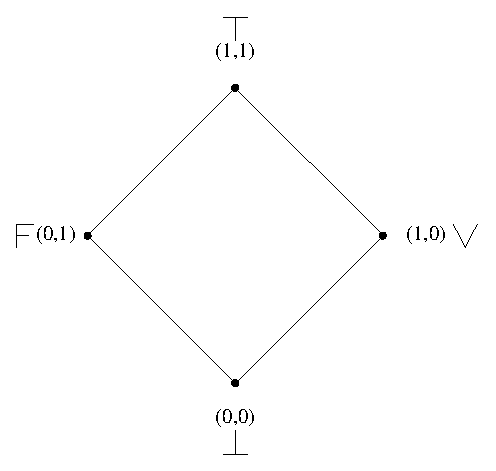
\includegraphics[scale=1.0]{./imagens/C421reticuladoHasse.eps}
%\label{fig:reticuladoHasse1}
%{\small Fonte: \cite{JoaoInacio} }
%\end{figure}


\begin{figure}[!h]
\centering
\caption{Representação do reticulado finito de Hasse }
\begin{tikzpicture}[scale=0.6]
\tikzset{ >=latex, inner sep=0pt, outer sep=0pt,  }

%\draw [lightgray, dashed](0,0) grid (10,10);

\node at (5.0,9.5) {$(1,1)$};
\node at (9.9,4.8) {$(1,0)$};
\node at (5.0,0.5) {$(0,0)$};
\node at (0.1,4.8) {$(0,1)$};

\node at (5.0,10.2) {$\top$};
\node at (9.9,5.5) {V};
\node at (5.0,-0.2) {$\bot$};
\node at (0.1,5.5) {F};

\node [fill=black, circle] (V) at (9,5) {:};
\node [fill=black, circle] (F) at (1,5) {:};
\node [fill=black, circle] (T) at (5,9) {:};
\node [fill=black, circle] (L) at (5,1) {:};

\draw [thick] (V) -- (T);
\draw [thick] (T) -- (F);
\draw [thick] (F) -- (L);
\draw [thick] (L) -- (V);

\end{tikzpicture}
\label{fig:reticuladoHasse}

{\small Fonte: \cite{JoaoInacio}}
\end{figure}








Para toda proposição $P$ há um par de valores, chamada de anotação, $(\mu , \lambda )$, onde $\mu$ é o grau de evidência favorável e $\lambda $ é o grau de evidência contrária, representada como  $P_{( \mu , \lambda )}$ \cite{Abe2014} .

%$P_{( \mu , \lambda )}$
Como exemplificação, para uma proposição $P \equiv$ \emph{"A velocidade de rotação do motor atingiu o valor desejado."}, assume-se dois especialistas para realizarem a leitura dos valores da anotação. Em um sistema físico, os especialistas geralmente são sensores, como neste caso, poderia ser um encoder ou sensor óptico como contador de voltas associado a uma base de tempo.

\begin{itemize}
\item 
$\mu$ = grau de evidência favorável (especialista 1), ou seja, com quanto de certeza, em um intervalo fechado $[0,1]$, sendo 0 para grau nulo de certeza e 1 grau máximo de certeza para a dada proposição $P$;

\item
$\lambda$ = grau de evidência contrária (especialista 2), ou seja, com quanto de certeza, em um intervalo fechado $[0,1]$, sendo 0 o grau nulo de certeza à evidência contrária e 1 o grau máximo de certeza à evidência contrária para a dada proposição $P$.

\end{itemize}


Assim, podemos interpretar da seguinte forma os valores da anotação para as posições extremas do reticulado finito de Hasse:

\begin{itemize}
\item 
$(\mu, \lambda ) = (1,0)$ : Há um grau de evidência favorável total e um grau de evidencia contrária nulo, ou seja, a afirmação da proposição é máxima e sua negação é nula, assim,  $P$ é \emph{Verdadeira} e \emph{A velocidade de rotação do motor atingiu o valor desejado};

\item 
$(\mu, \lambda ) = (0,1)$ : Há um grau de evidência favorável nulo e um grau de evidencia contrária máximo, ou seja, a afirmação da proposição é nula e sua negação é máxima, assim,  $P$ é \emph{Falsa} e \emph{A velocidade de rotação do motor não atingiu o valor desejado};

\item 
$(\mu, \lambda ) = (1,1)$ : Há um grau de evidência favorável máximo e também um grau de evidencia contrária máximo, ou seja, a afirmação da proposição é máxima e sua negação também é máxima, assim,  $P$ é \emph{Inconsistente} e \emph{A velocidade de rotação do motor atingiu e não atigiu o valor desejado}, contradição;

\item 
$(\mu, \lambda ) = (0,0)$ : Há um grau de evidência favorável nulo e também um grau de evidencia contrária nulo, ou seja, a afirmação da proposição é nula e sua negação também é nula, assim,  $P$ é \emph{Indeterminada} e \emph{A velocidade de rotação do motor nem atingiu o valor desejado e nem não atingiu o valor desejado}, situação paracompleta.

\end{itemize}

Os graus de evidência podem assumir valores não extremos:

\begin{itemize}
\item 
$(\mu, \lambda ) = (0.8,0.3)$ : Crê-se com grau de evidência favorável de 80\% e um grau de evidencia contrária de 30\%  que \emph{A velocidade rotação do motor atingiu do valor desejado}.
\end{itemize}

\subsubsection{Operações Lógicas}

Algumas operações lógicas booleanas são definidas 
a partir de duas anotações 
$(\mu _1, \lambda _1)$ e $(\mu _2, \lambda _2)$ 
pertencentes a mesma proposição P 
\cite{JISFeAS} \cite{Abe2014},
aqui denominadas respectivamente $P_1$ e $P_2$:

\begin{itemize}

\item Negação: $\sim$$P _1$ = $(\lambda _1, \mu _1)$ ou 
$\neg$$P _1$ = $(\lambda _1, \mu _1)$

\item Disjunção: $P _1 \vee P _2 = 
(min\{\mu _1, \mu _2\},max\{\lambda _1, \lambda _2\})$ 

\item Conjunção: $P _1 \wedge P _2 = 
(max\{\mu _1, \mu _2\},min\{\lambda _1, \lambda _2\})$ 


\end{itemize}




%%%%%%%%%%%%%%%%%%%%%%%%%%%%%%%%%%%%%%%%%%%%%%%%%%%%%%%%%%%%
\subsection{Quadrado Unitário no Plano Cartesiano - QUPC}
%%%%%%%%%%%%%%%%%%%%%%%%%%%%%%%%%%%%%%%%%%%%%%%%%%%%%%%%%%%%
\nomenclature{$QUPC$}{Quadrado Unitário no Plano Cartesiano}

Uma outra forma de representação da anotação é utilizando o Quadrado Unitário no Plano Cartesiano (QUPC) no qual são transpostos os pontos extremos às respectivas posições de acordo com o par ordenado,  $(\mu, \lambda ) \leftrightarrow (x,y) $, assim o eixo $x$ corresponde ao grau de evidência favorável e o eixo $y$ corresponde ao grau de evidência contrária, conforme mostrado na Figura \ref{fig:reticuladoQUPC}.




%\begin{figure}[!htb]
%\caption{Representação do reticulado no quadrado unitário no plano cartesiano}
%\center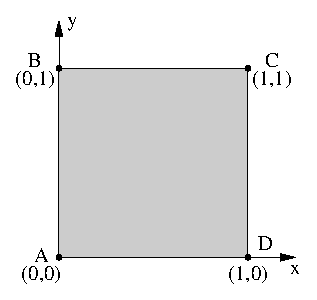
\includegraphics[scale=1.0]{./imagens/C422qupc.eps}
%\label{fig:reticuladoQUPC1}
%
%{\small Fonte: \cite{JoaoInacio} }
%\end{figure}


\begin{figure}[!h]
\centering
\caption{Representação do reticulado no quadrado unitário no plano cartesiano}
\begin{tikzpicture}[scale=0.6]
\tikzset{ >=latex, inner sep=0pt, outer sep=0pt,  }

%\draw [lightgray, dashed](0,0) grid (10,10);

\node at (1.2,9.4) {$y$};
\node at (9.4,0.8) {$x$};

\node at (0.0,0.3) {$(0,0)$};%A
\node at (0.0,7.5) {$(0,1)$};%B
\node at (9.0,7.5) {$(1,1)$};%C
\node at (8.0,0.3) {$(1,0)$};%D

\node at (0.0,1.1) {A};
\node at (0.0,8.5) {B};
\node at (8.5,8.5) {C};
\node at (8.5,1.5) {D};

\node [fill=black, circle] (V) at (8,1) {:};
\node [fill=black, circle] (F) at (1,8) {:};
\node [fill=black, circle] (T) at (8,8) {:};
\node [fill=black, circle] (L) at (1,1) {:};

\draw [thick] (V) -- (T);
\draw [thick] (T) -- (F);
\draw [thick] (F) -- (L);
\draw [thick] (L) -- (V);

\draw [->, thick] (0.8,1.0) -- (9.0,1.0);
\draw [->, thick] (1.0,0.8) -- (1.0,9.0);

\end{tikzpicture}
\label{fig:reticuladoQUPC}

{\small Fonte: \cite{JoaoInacio} }
\end{figure}







Os pontos extremos assim representam:

\begin{itemize}
\item $A: (0,0) = \bot \Rightarrow $ Paracompleto;
\item $B: (0,1) = F \Rightarrow $ Falso;
\item $C: (1,1) = \top \Rightarrow $ Inconsistente;
\item $D: (1,0) = V \Rightarrow $ Verdade.
\end{itemize}

O segmento de reta $\overline{BD}$, entre os pontos referentes às condições $Verdade$ e $Falso$, conforme mostrado na Figura \ref{fig:retaPerfeitamenteDefinida}, é denominada de \emph{Reta Perfeitamente Definida} e dada uma anotação $(\mu, \lambda )$ situada nela, a soma das evidências anotadas é sempre o valor unitário do quadro. 

%\begin{figure}[!htb]
%\caption{Representação da Reta Perfeitamente Definida}
%\center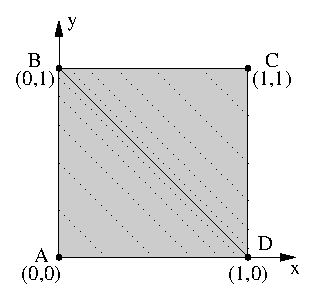
\includegraphics[scale=1.25]{./imagens/C424retaPerfeitamenteDefinida.eps}
%\label{fig:retaPerfeitamenteDefinida1}
%
%{\small Fonte: \cite{JoaoInacio}}
%\end{figure}

\begin{figure}[!h]
\centering
\caption{Representação da Reta Perfeitamente Definida}
\begin{tikzpicture}[scale=0.6]
\tikzset{ >=latex, inner sep=0pt, outer sep=0pt,  }

%\draw [lightgray, dashed](0,0) grid (10,10);

\node at (1.2,9.4) {$\lambda$};
\node at (9.4,0.8) {$\mu$};

\node at (0.0,0.3) {$(0,0)$};%A
\node at (0.0,7.5) {$(0,1)$};%B
\node at (9.0,7.5) {$(1,1)$};%C
\node at (8.0,0.3) {$(1,0)$};%D

\node at (0.0,1.1) {A};
\node at (0.0,8.5) {B};
\node at (8.5,8.5) {C};
\node at (8.5,1.5) {D};

\draw [gray,thick] (V) -- (T);
\draw [gray,thick] (T) -- (F);
\draw [gray,thick] (F) -- (L);
\draw [gray,thick] (L) -- (V);
\draw [] (F) -- (V);

\draw [->,gray, thick] (0.8,1.0) -- (9.0,1.0);
\draw [->,gray, thick] (1.0,0.8) -- (1.0,9.0);

\node [fill=black, circle] (V) at (8,1) {:};
\node [fill=black, circle] (F) at (1,8) {:};
\node [fill=black, circle] (T) at (8,8) {:};
\node [fill=black, circle] (L) at (1,1) {:};

\end{tikzpicture}
\label{fig:retaPerfeitamenteDefinida}

{\small Fonte: \cite{JoaoInacio}}
\end{figure}








A relação dos graus de evidência da anotação quando coincidente à Reta Perfeitamente Definida é: 

\begin{center}
\begin{equation}
\mu + \lambda = 1
\label{eq:evidenciaUnitaria1}
\end{equation}
\end{center}

Assim, temos que:

\begin{center}
\begin{equation}
\mu + \lambda - 1 = 0
\label{eq:evidenciaUnitaria}
\end{equation}
\end{center}


Os graus de evidência não precisam apresentar valores complementares, possuem independência entre si, assim das Equações  
\ref{eq:evidenciaUnitaria1} e 
\ref{eq:evidenciaUnitaria} 
é elaborado o conceito de 
\emph{Grau de Incerteza}($G_{in}$), 
e temos que: 

\nomenclature{$G_{in}$}{Grau de Incerteza}

\begin{center}
\begin{equation}
G_{in} = \mu + \lambda - 1
\label{eq:grauContradicao}
\end{equation}
\end{center}

pois quanto mais próximo da Reta Perfeitamente Definida, menor é o grau de incerteza apresentado pelos graus de evidência, sendo zero quando não houver inconsistência e o ponto de anotação situar-se sobre a Reta Perfeitamente Definida. 
Quanto mais afastado da Reta Perfeitamente Definida estiver o ponto de anotação, e mais próximo aos pontos A ou C, maior é o Grau de Incerteza. 

Quando a anotação estiver situada na região entre os pontos BCD, acima da reta perfeitamente definida, o Grau de Incerteza é denominado 
\emph{Grau de Inconsistência} ($G_{ic}$), 
e isso ocorre quando, $\mu \ge \lambda $, de forma oposta, quando $\mu < \lambda $ a anotação está situada na região entre os pontos BAD, abaixo da reta perfeitamente definida, e o grau de Incerteza é denominado 
\emph{Grau de Paracompleteza} ($G_{pa}$), 
então pode-se dizer que:

\nomenclature{$G_{pa}$}{Grau de Paracompleteza}
\nomenclature{$G_{ic}$}{Grau de Inconsistência}

\begin{center}
\begin{equation}
-1 \le G _{pa}  <  0 \le G _{ic} \le 1
\label{eq:grauInconsistenciaIndefinicao}
\end{equation}
\end{center}
e
\begin{center}
\begin{equation}
-1 \le G _{in} \le 1
\label{eq:grauInconsistenciaIndefinicao1}
\end{equation}
\end{center}


O segmento de reta $\overline{ AC }$ , entre os pontos referentes às
condições \emph{Paracompletude} e \emph{Inconsistência}, conforme mostrado
na Figura \ref{fig:retaPerfeitamenteIndefinida}, é denominada de
\emph{Reta Perfeitamente Indefinida} e dada uma anotação $(\mu,
\lambda )$ situada nela, a subtração das evidências anotadas é sempre
zero, ou seja, $\mu = \lambda$, e de forma contrária,
quando a anotação está posicionada de forma não coincidente à Reta
Perfeitamente Indefinida,
significa que $\mu \neq \lambda$.

%\begin{figure}[!htb]
%\caption{Representação da Reta Perfeitamente Indefinida}
%\center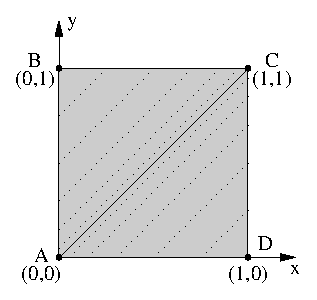
\includegraphics[scale=1.25]{./imagens/C426retaPerfeitamenteIndefinida.eps}
%\label{fig:retaPerfeitamenteIndefinida1}
%
%{\small Fonte: \cite{JoaoInacio} }
%\end{figure}



\begin{figure}[!h]
\centering
\caption{Representação da Reta Perfeitamente Indefinida}
\begin{tikzpicture}[scale=0.6]
\tikzset{ >=latex, inner sep=0pt, outer sep=0pt,  }

%\draw [lightgray, dashed](0,0) grid (10,10);

\node at (1.2,9.4) {$\lambda$};
\node at (9.4,0.8) {$\mu$};

\node at (0.0,0.3) {$(0,0)$};%A
\node at (0.0,7.5) {$(0,1)$};%B
\node at (9.0,7.5) {$(1,1)$};%C
\node at (8.0,0.3) {$(1,0)$};%D

\node at (0.0,1.1) {A};
\node at (0.0,8.5) {B};
\node at (8.5,8.5) {C};
\node at (8.5,1.5) {D};

\draw [gray,thick] (V) -- (T);
\draw [gray,thick] (T) -- (F);
\draw [gray,thick] (F) -- (L);
\draw [gray,thick] (L) -- (V);
\draw [thick] (T) -- (L);

\draw [->,gray, thick] (0.8,1.0) -- (9.0,1.0);
\draw [->,gray, thick] (1.0,0.8) -- (1.0,9.0);

\node [fill=black, circle] (V) at (8,1) {:};
\node [fill=black, circle] (F) at (1,8) {:};
\node [fill=black, circle] (T) at (8,8) {:};
\node [fill=black, circle] (L) at (1,1) {:};

\end{tikzpicture}
\label{fig:retaPerfeitamenteIndefinida}

{\small Fonte: \cite{JoaoInacio} }
\end{figure}











A relação dos graus de evidência para uma anotação cuja posição coincide com a Reta Perfeitamente Indefinida é: 

\begin{center}
\begin{equation}
\mu - \lambda = 0
\label{eq:evidenciaIndefinida}
\end{equation}
\end{center}

De forma análoga ao Grau de Inconsistência, da Equação \ref{eq:evidenciaIndefinida} é elaborado o conceito de \emph{Grau de Certeza} ($G_{ce}$), assim temos que: 

\nomenclature{$G_{ce}$}{Grau de Certeza}

\begin{center}
\begin{equation}
G _{ce} = \mu - \lambda
\label{eq:grauCerteza}
\end{equation}
\end{center}

Quando os graus de evidência, favorável e contrário, são iguais, não há certeza em relação à proposição, mas quando são diferentes, alguma certeza pode ser inferida, até a condição máxima onde uma das evidências é total (1) e a outra é nula (0), caracterizando a condição verdadeira ou falsa, afastando o ponto anotado da Reta Perfeitamente Indefinida. 

Quando a anotação situa-se entre os pontos ABC do QUPC, o grau de certeza é denominado \emph{Grau de Falsidade ($G _{fa}$)}, e tal condição ocorre quando $\mu < \lambda $, caso contrário, se $\mu \ge \lambda $, a anotação situa-se entre os pontos ACD do QUPC, e o grau de certeza é denominado \emph{Grau de Veracidade ($G _{ve})$}, então pode-se dizer que:

\nomenclature{$G_{fa}$}{Grau de Falsidade}
\nomenclature{$G_{ve}$}{Grau de Veracidade}

\begin{center}
\begin{equation}
-1 \le G_{fa}  <  0 \le G_{ve} \le 1
\label{eq:grauVerdadeFalsidade}
\end{equation}
\end{center}
e
\begin{center}
\begin{equation}
-1 \le G_{ce} \le 1
\label{eq:grauCertezaIntervalo}
\end{equation}
\end{center}

Graficamente são representadas como mostra a Figura \ref{fig:retasgcgct}:

%\begin{figure}[!htb]
%\caption{Representação dos Graus de Certeza e Incerteza em um plano cartesiano}
%\center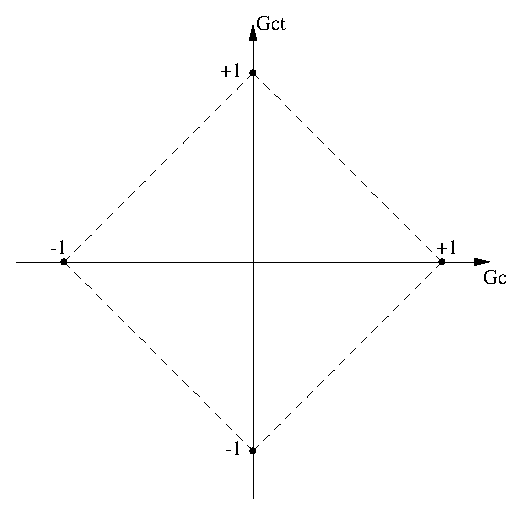
\includegraphics[scale=1.0]{./imagens/C428retasgcgct.eps}
%\label{fig:retasgcgct1}
%
%{\small Fonte: \cite{JoaoInacio}}
%\end{figure}

\begin{figure}[!h]
\centering
\caption{Representação dos Graus de Certeza e Incerteza em um plano cartesiano}
\begin{tikzpicture}[scale=0.8]
\tikzset{ >=latex, inner sep=0pt, outer sep=0pt,  }

%\draw [lightgray, dashed](0,0) grid (10,10);

\node at ( 5.5,10.0) {$G_{in}$};
\node at (10.0, 5.5) {$G_{ce}$};

\node at (9.0,4.5) {$+1$};
\node at (0.5,5.5) {$-1$};
\node at (4.5,9.4) {$+1$};
\node at (4.5,0.6) {$-1$};

\draw [->,gray, thick] (5.0,0.0) -- ( 5.0,10.0);
\draw [->,gray, thick] (0.0,5.0) -- (10.0, 5.0);

\node [fill=black, circle] (V) at (9,5) {.};
\node [fill=black, circle] (F) at (1,5) {.};
\node [fill=black, circle] (T) at (5,9) {.};
\node [fill=black, circle] (L) at (5,1) {.};

\draw [dashed] (V)--(T);
\draw [dashed] (T)--(F);
\draw [dashed] (F)--(L);
\draw [dashed] (L)--(V);

\end{tikzpicture}
\label{fig:retasgcgct}

{\small Fonte: \cite{JoaoInacio}}
\end{figure}











A representação ainda é dividia em algumas partes, dependendo da aplicação, estabelecendo quais são os limites que definem cada estado, Verdadeiro, Falso, Paracompleto, Inconsistente e outros mais que forem pertinentes à aplicação, estão representados pelas linhas tracejadas na Figura \ref{fig:valorControle} e são definidos como:

\begin{itemize}
\item \emph{$V_{scc}$ : Valor limite superior de Controle de Certeza};
\item \emph{$V_{icc}$ : Valor limite inferior de Controle de Certeza};
\item \emph{$V_{sci}$ : Valor limite superior de Controle de Incerteza};
\item \emph{$V_{ici}$ : Valor limite inferior de Controle de Incerteza}.
\end{itemize}

\nomenclature{$V_{scc}$}{ Valor limite superior de controle de certeza}
\nomenclature{$V_{icc}$}{ Valor limite inferior de controle de certeza}
\nomenclature{$V_{sci}$}{ Valor limite superior de controle de incerteza}
\nomenclature{$V_{ici}$}{ Valor limite inferior de controle de incerteza}


%\begin{figure}[!htb]
%\caption{Representação dos valores de controle}
%\center\includegraphics[scale=1.0]{./imagens/C429valorControle.eps}
%\label{fig:valorControle1}
%
%{\small Fonte: \cite{JoaoInacio}}
%\end{figure}

\begin{figure}[!h]
\centering
\caption{Representação dos valores de controle}
\begin{tikzpicture}[scale=0.8]
\tikzset{ >=latex, inner sep=0pt, outer sep=0pt,  }

%\draw [lightgray, dashed](0,0) grid (10,10);

\node at ( 5.5,10.0) {$G_{in}$};
\node at (10.0, 5.5) {$G_{ce}$};

\node at (9.0,4.5) {$+1$};
\node at (0.5,5.5) {$-1$};
\node at (4.5,9.4) {$+1$};
\node at (4.5,0.6) {$-1$};

\draw [->, thick] (5.0,0.0) -- ( 5.0,10.0);
\draw [->, thick] (0.0,5.0) -- (10.0, 5.0);

\node [fill=black, circle] (V) at (9,5) {.};
\node [fill=black, circle] (F) at (1,5) {.};
\node [fill=black, circle] (T) at (5,9) {.};
\node [fill=black, circle] (L) at (5,1) {.};

\draw [thick] (V)--(T);
\draw [thick] (T)--(F);
\draw [thick] (F)--(L);
\draw [thick] (L)--(V);

\draw [dashed] (7,7)--(3,7)--(3,3)--(7,3)--(7,7);

\end{tikzpicture}
\label{fig:valorControle}

{\small Fonte: \cite{JoaoInacio}}
\end{figure}














Uma divisão em 12 partes é mostrada na Figura \ref{fig:reticuladoLPA2v} com seus respectivos estados intermediários definidos conforme \citeauthor{JoaoInacio}(\citeyear{JoaoInacio}), sendo 4 regiões extremas:


%\begin{figure}[!htb]
%\center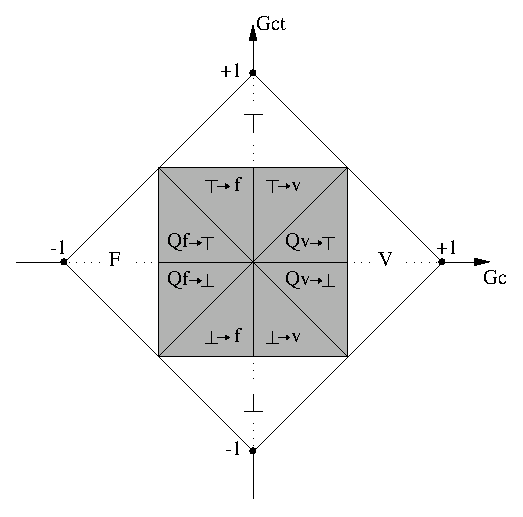
\includegraphics[scale=1.5]{./pic/C430gcgct.eps}
%\caption{Representação do reticulado da LPA2v subdividido em 12 regiões}
%\label{fig:reticuladoLPA2v}
%\end{figure}


\begin{figure}[!h]
\centering
\caption{Representação do reticulado da Lógica $E\tau$ subdividido em 12 regiões}
\begin{tikzpicture}[scale=1.0]
\tikzset{ >=latex, inner sep=0pt, outer sep=0pt,  }

%\draw [lightgray, dashed](0,0) grid (10,10);

\node [fill=black, circle] (V) at (9,5) {:};
\node [fill=black, circle] (F) at (1,5) {:};
\node [fill=black, circle] (T) at (5,9) {:};
\node [fill=black, circle] (L) at (5,1) {:};

\node [fill=black, circle] (N) at (5,7) { };
\node [fill=black, circle] (S) at (5,3) { };
\node [fill=black, circle] (E) at (7,5) { };
\node [fill=black, circle] (W) at (3,5) { };

\node [fill=black, circle] (NE) at (7,7) { };
\node [fill=black, circle] (SE) at (7,3) { };
\node [fill=black, circle] (NW) at (3,7) { };
\node [fill=black, circle] (SW) at (3,3) { };


%\draw [dashed] (F) -- (V);
%\draw [dashed] (T) -- (L);
\draw [->, thick] (V)   -- (10,5);
\draw [    thick] (0,5) -- (F);
\draw [->, thick] (T)   -- (5,10);
\draw [    thick] (5,0) -- (L);

\draw [thick] (V) -- (T);
\draw [thick] (T) -- (F);
\draw [thick] (F) -- (L);
\draw [thick] (L) -- (V);

\draw [thick] (N) -- (S);
\draw [thick] (E) -- (W);
\draw [thick] (NE) -- (SW);
\draw [thick] (SE) -- (NW);


\draw[thick] (SW) rectangle (NE);
\fill[nearly transparent] (SW) rectangle (NE);

\node at (8,5) {V};
\node at (2,5) {F};
\node at (5,8) {$\top$};
\node at (5,2) {$\bot$};

\node at (6.2,5.3) {Qv$\rightarrow\top$ };
\node at (6.2,4.7) {Qv $\rightarrow  \bot$ };
\node at (3.8,5.3) {Qf $\rightarrow  \top$ };
\node at (3.8,4.7) {Qf $\rightarrow  \bot$ };
\node at (4.2,6.6) {$\top \rightarrow $ f };
\node at (5.8,6.6) {$\top \rightarrow $ v };
\node at (4.2,3.4) {$\bot \rightarrow $ f };
\node at (5.8,3.4) {$\bot \rightarrow $ v };

\node at (10,4.5) {$G_{ce}$};
\node at (5.5,10) {$G_{in}$};

\node at (4.5,9.2) {$+1$};
\node at (9.0,5.5) {$+1$};
\node at (5.5,1.0) {$-1$};
\node at (1.0,4.5) {$-1$};

\end{tikzpicture}
\label{fig:reticuladoLPA2v}

{\small Fonte: \cite{JoaoInacio} }
\end{figure}




\begin{itemize}
\item V : Verdadeiro;
\item F : Falso;
\item $\top$ : Inconsistente;
\item $\bot$ : Paracompleto.
\end{itemize}
e 8 regiões intermediárias: 
\begin{itemize}
\item Qv $\rightarrow  \top$ : Quase Verdade tendendo à Inconsistência;
\item Qv $\rightarrow  \bot$ : Quase Verdade tendendo à  Paracompletude;
\item Qf $\rightarrow  \top$ : Quase Falso tendendo à Inconsistência;
\item Qf $\rightarrow  \bot$ : Quase Falso tendendo à Paracompletude;
\item $\top \rightarrow $ f : Inconsistência tendendo à Falsidade;
\item $\top \rightarrow $ v : Inconsistência tendendo à Veracidade;
\item $\bot \rightarrow $ f : Paracompleto tendendo à Falsidade;
\item $\bot \rightarrow $ v : Paracompleto tendendo à Veracidade.

\end{itemize}

O reticulado subdividido em 12 regiões como mostrado, é aplicado em situações nas quais a tomada de decisão utiliza estados discretos bem definidos para atuação, onde para cada posição da anotação e respectivamente um estado do reticulado, uma ação é tomada, assim sendo, a quantidade de subdivisões está fortemente dependente da aplicação.


O reticulado pode ser dividido de outras formas, dependendo dos limites dos Graus de Certeza e Incerteza que o sistema permite. A Figura \ref{fig:reticuladoLPA2v2} mostra uma das possibilidades com a representação de 8 regiões do reticulado. 


\begin{figure}[!h]
\centering
\caption{Representação do reticulado da Lógica $E\tau$ subdividido em 8 regiões}
\begin{tikzpicture}[scale=1.0]
\tikzset{ >=latex, inner sep=0pt, outer sep=0pt,  }

%\draw [lightgray, dashed](0,0) grid (10,10);

\node at (10,4.5) {$G_{ce}$};
\node at (5.5,10) {$G_{in}$};

\node at (4.5,9.2) {$+1$};
\node at (9.0,5.5) {$+1$};
\node at (5.5,1.0) {$-1$};
\node at (1.0,4.5) {$-1$};

\node [fill=black, circle] (V) at (9,5) {:};
\node [fill=black, circle] (F) at (1,5) {:};
\node [fill=black, circle] (T) at (5,9) {:};
\node [fill=black, circle] (L) at (5,1) {:};

\node [fill=black, circle] (N) at (5,7) { };
\node [fill=black, circle] (S) at (5,3) { };
\node [fill=black, circle] (E) at (7,5) { };
\node [fill=black, circle] (W) at (3,5) { };

\node [fill=black, circle] (NE) at (8,6) { };
\node [fill=black, circle] (SE) at (8,4) { };
\node [fill=black, circle] (NW) at (2,6) { };
\node [fill=black, circle] (SW) at (2,4) { };

\draw [->, thick] (V)   -- (10,5);
\draw [    thick] (0,5) -- (F);
\draw [->, thick] (T)   -- (5,10);
\draw [    thick] (5,0) -- (L);

\draw [thick] (V) -- (T);
\draw [thick] (T) -- (F);
\draw [thick] (F) -- (L);
\draw [thick] (L) -- (V);

\draw [thick] (NE) -- (SW);
\draw [thick] (SE) -- (NW);

\draw[thick] (SW) rectangle (NE);
\fill[nearly transparent] (SW) rectangle (NE);

\node at (8.5,5.0) {V};
\node at (1.5,5.0) {F};
\node at (5.0,8.0) {$\top$};
\node at (5.0,2.0) {$\bot$};

\node at (7.0,5.0) {Qv};
\node at (3.0,5.0) {Qf};
\node at (5.0,5.5) {Q$\top$};
\node at (5.0,4.5) {Q$\bot$};

\end{tikzpicture}
\label{fig:reticuladoLPA2v2}

{\small Fonte: Próprio autor}
\end{figure}

Sendo 4 regiões extremas,
\begin{itemize}
\item V : Verdadeiro;
\item F : Falso;
\item $\top$ : Inconsistente;
\item $\bot$ : Paracompleto.
\end{itemize}
e 4 regiões intermediárias: 
\begin{itemize}
\item Qv: Quase Verdade;
\item Qf: Quase Falso;
\item Q$\top$: Quase Inconsistente;
\item Q$\bot$: Quase Paracompleto.

\end{itemize}


%###

É possível e desejável que se possa utilizar um valor resultante que
exclua os efeitos das paracompletudes ou inconsistências \cite{JairJoaoGermano}:

\begin{citacao}
{
"Um sistema de decisão capaz de analisar dados originários de Conhecimento Incerto terá maior robustez quando, 
ao final da análise,
apresentar um resultado que represente o valor de certeza puro, 
isto é, não contaminado pelos efeitos das incertezas."
}
\end{citacao}

O valor que elimina o efeito da incerteza é denominado \emph{Grau de Certeza Real - $G_{CR}$} 
e é calculado pela distância (D) do Ponto de análise, $(G_{ce},G_{in})$, 
em relação ao ponto de máximo Grau de Certeza $V$,
no vértice direito do reticulado, 
conforme mostrado na Figura \ref{fig:reticuladoGer}.

\nomenclature{$G_{CR}$}{Grau de Certeza Real}

\begin{figure}[!h]
\centering
\caption{Representação do Grau de Certeza Real no reticulado }
\begin{tikzpicture}[scale=1.0]
\tikzset{ >=latex, inner sep=0pt, outer sep=0pt,  }

%\draw [lightgray, dashed](0,0) grid (10,10);

\node at (10,4.5) {$G_{ce}$};
\node at (5.5,10) {$G_{in}$};

\node at (4.5,9.2) {$+1$};
\node at (9.0,5.5) {$+1$};
\node at (5.5,1.0) {$-1$};
\node at (1.0,4.5) {$-1$};

\node at (9.0,4.5) {V};
\node at (1.0,5.5) {F};
\node at (5.5,9.0) {$\top$};
\node at (4.5,1.0) {$\bot$};

\node [fill=black, circle] (V) at (9,5) {:};
\node [fill=black, circle] (F) at (1,5) {:};
\node [fill=black, circle] (T) at (5,9) {:};
\node [fill=black, circle] (L) at (5,1) {:};

\draw [thick] (V) -- (T);
\draw [thick] (T) -- (F);
\draw [thick] (F) -- (L);
\draw [thick] (L) -- (V);

\draw [->, thick] (V)   -- (10,5);
\draw [    thick] (0,5) -- (F);
\draw [->, thick] (T)   -- (5,10);
\draw [    thick] (5,0) -- (L);

\draw [lightgray,dashed] (V) -- (F);
\draw [lightgray,dashed] (T) -- (L);

\node [fill=black, circle] (P) at (6.0,7.0) {:};
\node [fill=gray,  circle] (p) at (5.4,5.0) [gray] {:};
\node [fill=black, circle] (r) at (6.0,5.0) [gray]{.};

\draw [blue,ultra thick] (P) -- (V);
\draw [green ] (r) -- (V);
\draw [yellow] (P) -- (r);
%\draw [green,ultra thick] (9.0,4.9) -- (5.4,4.9);

\draw [red, ultra thick,<-]  (p) to [out=85, in=236] (P);

\node at (7.0,6.0) [blue]{D};
\node at (5.7,7.4) {($G_{ce}$,$G_{in}$)};
\node at (5.5,4.6) {$G_{CR}$};

\end{tikzpicture}
\label{fig:reticuladoGer}

{\small Fonte: \cite{JairJoaoGermano}}
\end{figure}


O Grau de Certeza Real ($G_{CR}$) 
é calculado utilizando o Teorema de Pitágoras para achar a distância D 
conforme Equação \ref{eq:grauCertezaReal}. 

\begin{center}
\begin{equation}
D = \sqrt{(1-|G_{ce}|)^2+G_{in}^2}
\label{eq:grauCertezaReal}
\end{equation}
\end{center}

Para valores de $G_{ce} \geq 0$: 

\begin{center}
\begin{equation}
G_{CR} = (1-D)
\end{equation}
\end{center}

Para valores de $G_{ce} < 0$:

\begin{center}
\begin{equation}
G_{CR} = (D-1)
\end{equation}
\end{center}


O Grau de Evidência Real é representado por $\mu_{ER}$ 
e é utilizado para converter o $G_{ce}$ ou $G_{CR}$ 
em uma variável dentro do intervalo fechado $[0,1]$, 
permitindo que o resultado de um bloco LPA$E\tau$ 
possa ser utilizado como entrada em outro bloco. 
Para a conversão é efetuada a equação \ref{eq:muer}:

%\nomenclature{$\mu_{ER}$}{Grau de Evidência Real}

\begin{equation}
\mu_{ER} = \frac{G_{ce} + 1}{2}
\label{eq:muer}
\end{equation}


Tanto o Grau de Certeza Real quanto o Grau de Evidência Real 
ou os estados ou regiões do reticulado 
podem ser utilizados para realizar o controle dos mais diversos tipos de sistemas, 
dependendo apenas do tipo de controle e de sistema que deve ser implementado. 




\chapter[Desenvolvimento]{3. Desenvolvimento}
%%%%%%%%%%%%%%%%%%%%%%%%%%%%%%%%%%%%%%%%%%%%%%%%%%%%%%%%%%%%
%%%%%%%%%%%%%%%%%%%%%%%%%%%%%%%%%%%%%%%%%%%%%%%%%%%%%%%%%%%%
%\section{A proposição e a anotação}

Como ponto de partida,
é definida uma proposição como sendo a variável manipulada em seu valor máximo.
Como o sistema proposto neste trabalho tem um controle de motor de corrente contínua,
sendo a tensão média aplicada ao motor, para controle da sua velocidade,
através de um acionamento do tipo modulação por largura de pulso (\emph{PWM}),
cujo parâmetro é o \emph{duty cycle}, ou seja, o percentual em que o nível lógico
da modulação está atuando,
assim, quando a variável manipulada for máxima,
significa que a proposição alcançou a verdade.
Pode-se então definir a proposição como sendo:
"P: O acionamento do motor está ajustado para velocidade máxima."

A velocidade de rotação do motor é a variável controlada,
e a sua relação com a variável manipulada se dá pela relação direta
no processo de calibração do controlador,
em que a velocidade máxima do sistema é definida como ponto de verdade do reticulado.
Assim, o controlador opera como um sistema em malha aberta,
ajustando a variável manipulada para o máximo,
deve-se obter o máximo da variável controlada,
definindo assim o ponto de verdade do reticulado.
De forma análoga, ajustando a variável manipulada para o mínimo,
normalmente zero, deve-se obter o mínimo da variável controlada,
velocidade zero, ponto de falsidade do reticulado.

Como os pontos de verdade e falsidade definem os respectivos de
máxima e mínima da variável controlada, velocidade de rotação do motor,
toda extensão de velocidades está contida sobre a reta perfeitamente definida,
assim a reta do grau de certeza contém todas as possibilidades de velocidade,
dado um erro zero entre valor desejado, valor de referência ou \emph{set point},
e o valor lido pelo sensor de velocidade, variável controlada.

O valor desejado então é representado pelo grau de evidência favorável ($\mu$),
enquanto que o complemento do valor do sensor é o grau de evidência contrário ($\lambda$).
Como o $\lambda$ é o complemento do sensor,
pode-se assumir o sensor como um segundo segundo grau de evidência favorável.
Assim adota-se $\mu_0 = \mu$ e $\mu_1 = (1 - \lambda)$.



O diagrama da Figura \ref{fig:diagramaBlocosLPAEt} apresenta 
a planta do sistema $g(t)$ tendo como saída a 
variável controlada $c(t)$, 
que é a velocidade de rotação do disco 
acoplado ao eixo do motor, 
e como entrada a variável manipulada $u(t)$, 
que é o parâmetro do \emph{PWM} 
que produz a sinal aplicado à planta.



\begin{figure}[!h]%%%%%%%%%%%%%%%%%%%%%%%%%%%%%%%%fg
\centering
\caption{Diagrama de blocos do controle utilizando a LPA$E\tau$}
\begin{tikzpicture}[scale=1.0]
\tikzset{ >=latex, inner sep=0pt, outer sep=0pt,  }

%\draw [lightgray, dashed](0,0) grid (15,4.2);

%%% Blocos 

% Kn normalização rps -> 0..1
\node [fill=black, circle] (KSP0) at (2.0,4.0) { };
\node [fill=black, circle] (KSP1) at (3.0,3.0) { };
\draw[thick] (KSP0) rectangle (KSP1);
\fill[white, nearly transparent] (KSP0) rectangle (KSP1);
\node [fill=black, circle] (KSPin)  at (2.0,3.5) { }; 
\node [fill=black, circle] (KSPout) at (3.0,3.5) { }; 
\node (Kn1) at (2.5,3.5) {$K_n$};

% Kn Sensor
\node [fill=black, circle] (KS0) at (2.0,2.0) { };
\node [fill=black, circle] (KS1) at (3.0,1.0) { };
\draw[thick] (KS0) rectangle (KS1);
\fill[white, nearly transparent] (KS0) rectangle (KS1);
\node [fill=black, circle] (KSin)  at (2.0,1.5) { };
\node [fill=black, circle] (KSout) at (3.0,1.5) { };
\node (Kn2) at (2.5,1.5) {$K_n$};

% LPAEt
\node [fill=black, circle] (LPA0) at (4,4.0) { };
\node [fill=black, circle] (LPA1) at (7,1.0) { };
\draw[thick] (LPA0) rectangle (LPA1);
\fill[white, nearly transparent] (LPA0) rectangle (LPA1);
\draw [thick] (5.5,4.0) -- (7.0,2.5) -- (5.5,1.0) -- (4.0,2.5) -- (5.5,4.0);
\node (LPA2v) at (5.5,2.5) {$LPAE\tau$};
\node [fill=black, circle] (LPAu0)  at (4.0,3.5) { };
\node [fill=black, circle] (LPAu1)  at (4.0,1.5) { };
\node [fill=black, circle] (LPAgc)  at (7.0,3.5) { };
\node [fill=black, circle] (LPAs)   at (7.0,2.5) { };
\node [fill=black, circle] (LPAgct) at (7.0,1.5) { };
\node (LPA2vu0)  at (3.4,3.7) {$\mu _0$};
\node (LPA2vu1)  at (3.4,1.7) {$\mu _1$};

% Kn u(t)
\node [fill=black, circle] (KU0) at (8.0,3.0) { };
\node [fill=black, circle] (KU1) at (9.0,2.0) { };
\draw[thick] (KU0) rectangle (KU1);
\fill[white, nearly transparent] (KU0) rectangle (KU1);
\node [fill=black, circle] (KUin)  at (8.0,2.5) { };
\node [fill=black, circle] (KUout) at (9.0,2.5) { };
\node (Ku2) at (8.5,2.5) {$K_u$};


% Planta
\node [fill=black, circle] (GT0) at (10,4.0) { };
\node [fill=black, circle] (GT1) at (13,1.0) { };
\draw[thick] (GT0) rectangle (GT1);
\fill[white, nearly transparent] (GT0) rectangle (GT1);
\node [fill=black, circle] (GTin)  at (10.0,2.5) { };
\node [fill=black, circle] (GTout) at (13.0,2.5) { };
\node (planta) at (11.5,2.5) {$g(t)$};



%%% Linhas 

% set point
\draw [->, thick] (0.0,3.5) -- (KSPin);
\node (rt) at (1.0,3.8) {$r(t)$};

% GT -> fim
\draw [->, thick] (GTout) -- (15,2.5);
\node (ct) at (14.0,2.8) {$c(t)$};
\node (ct) at (1.0,1.8) {$c(t)$};

% normalização 0..1 -> LPA2v u0
\draw [->, thick] (KSPout) -- (LPAu0);

% normalização 0..1 -> LPA2v u1
\draw [->, thick] (KSout) -- (LPAu1);

% LPAEt -> Ku
\draw [->, thick] (LPAs) -- (KUin);
\node (ut) at (7.5,2.8) {$\mu_{ER}\delta$};

% Ku -> GT
\draw [->, thick] (KUout) -- (GTin);
\node (ut) at (9.5,2.8) {$u(t)$};

% GT -> Kn Sensor
\draw [->, thick] (GTout) -- (14.0,2.5) -- (14.0,0.0) -- (1.0,0.0) -- (1.0,1.5) -- (KSin);


\end{tikzpicture}
\label{fig:diagramaBlocosLPAEt}

{\vspace{0.2cm} \small Fonte: Próprio autor}
\end{figure}
%%%%%%%%%%%%%%%%%%%%%%%%%%%%%%%%%%%%%%%%



A variável manipulada $u(t)$ é produzida pelo 
bloco controlador $LPAE\tau$, 
e este recebe seus parâmetros no formato dos 
graus de evidência favoráveis $\mu_0$ e $\mu_1$.
Sendo o parâmetro $\mu_1$ 
convertido internamente em $\lambda$ 
como grau de evidência contrária.

Os dois parâmetros que vão gerar os graus de evidência 
possuem a mesma natureza, a mesma escala, 
são a velocidade desejada e a velocidade lida pelo sensor,
de modo a poder comparar e utilizá-las nas operações da
LPA$E\tau$. 
Para adequação da escala das grandezas 
de referência $r(t)$ e da variável controlada $c(t)$
ao intervalo de trabalho dos parâmetros da LPA$E\tau$, 
é inserido um bloco de normalização do sinal em cada entrada,
bem como na saída.


Para a normalização os blocos $K_n$ realizam as seguinte operações:

\begin{equation}%%%%%%%%%%%%%%%%%%%%%%%%%%%%%%%%%% eq
\mu_0 = \frac{ r(t)}{c(t)_{\text{máx}}} \ \ \ \ \ \ \ \ \mu_1 = \frac{c(t)}{c(t)_{\text{máx}}}
\label{eq:nomaliza}
\end{equation}%%%%%%%%%%%%%%%%%%%%%%%%%%%%%%%%%%%%
\vspace{-0.4cm}
onde:

$c(t)_{\text{máx}}$: é a velocidade máxima produzida pelo sistema.


Para a normalização do bloco $K_u$ é realizada a seguinte operação:

\begin{equation}
u(t) = \mu_{ER}\delta . 100
\end{equation}

\vspace{-0.4cm}
onde:

$\mu_{ER}\delta$: valor contido no intervalo fechado [0, 1].

$u(t)$: valor contido no intervalo [0, 100] 
referente ao parâmetro(\%) do acionamento PWM.




%%%%%%%%%%%%%%%%%%%%%%%%%%%%%%%%%%%%%%%%%%%%%%%%%%%%%%%%%%%%
%%%%%%%%%%%%%%%%%%%%%%%%%%%%%%%%%%%%%%%%%%%%%%%%%%%%%%%%%%%%
%\newpage

Tendo o $\mu_1 (\mu)$ e o $\mu_1 (1-\lambda)$ ajustados dessa forma,
tem-se que todas as possibilidades consideráveis estão contidas dentro do reticulado,
e a sua divisão em regiões é mandatória para a realização do controle e o tratamento de
falhas, mas que seus limiares vão depender intrinsecamente do sistema controlado.

As regiões aqui definidas para a realização do controle proposto
são expostas de forma incremental e complementar no reticulado,
definindo o controlador aqui proposto,
bem como as nomenclaturas para tal aplicação,
diferentes das implementações em trabalhos anteriores,
por ser uma abordagem diferenciada destes.


\section{Região de incerteza positiva e negativa}

A região de incerteza está contemplada em toda a região diferente da
reta perfeitamente definida, local em que o Grau de Incerteza vale zero,
tendo acima desta a denominação de região de incerteza positiva
enquanto que abaixo a denominação é região de incerteza negativa,
denominações que serão utilizados no reticulado para a aplicação
apresentada neste trabalho.


%%%%%%%%%%%%%%%%%%%%%%%%%%%%%%%%%%%%%%%%%%%%%%%%%%%%%%%%% Fg
\begin{figure}[!h]%%%%%%%%%%%%%%%%%%%%%%%%%%%%%%%%%%%%%%%%%%
\centering
\caption{Representação das regiões de incerteza não nulas (positiva e negativa)}
\begin{tikzpicture}[scale=0.80]
\tikzset{ >=latex, inner sep=0pt, outer sep=0pt,  }

%\draw [lightgray, dashed](0,0) grid (10,10);

\node [fill=black, circle] (V) at (9,5) {:};
\node [fill=black, circle] (F) at (1,5) {:};
\node [fill=black, circle] (T) at (5,9) {:};
\node [fill=black, circle] (L) at (5,1) {:};

\draw [->, thick] (V)   -- (10,5);
\draw [    thick] (0,5) -- (F);
\draw [->, thick] (T)   -- (5,10);
\draw [    thick] (5,0) -- (L);

\draw [thick] (V) -- (T);
\draw [thick] (T) -- (F);
\draw [thick] (F) -- (L);
\draw [thick] (L) -- (V);

\node at (10,4.5) {$G_{ce}$};
\node at (5.5,10) {$G_{in}$};

\node at (4.5,9.2) {$+1$};
\node at (9.0,5.5) {$+1$};
\node at (5.5,1.0) {$-1$};
\node at (1.0,4.5) {$-1$};

\node at (9.0,4.5) {V};
\node at (1.0,5.5) {F};
\node at (5.5,9.2) {$\top$};
\node at (4.5,1.0) {$\bot$};

\draw [fill, green,nearly transparent] (5.0,9.0) -- (1.0,5.0) -- (9.0,5.0) -- (5.0,9.0);
\draw [fill,  blue,nearly transparent] (5.0,1.0) -- (1.0,5.0) -- (9.0,5.0) -- (5.0,1.0);
\draw [white, thick] (1.0,5.0) -- (9.0,5.0);

\node at (9,8) {Região de Incerteza};
\node at (9,7) {Positiva};
\draw [->,thick] (7.5,7.6) -- (5.5,6);

\node at (1,2) {Região de Incerteza};
\node at (1,1) {Negativa};
\draw [->,thick] (2,2.5) -- (4,3.5);
%\draw [dashed, green] (8.5,5.5) -- (8.5,4.5);
\end{tikzpicture}
\label{fig:regiaoIncentezaPosNeg}

{\small Fonte: Próprio autor }
\end{figure}
%%%%%%%%%%%%%%%%%%%%%%%%%%%%%%%%%%%%%%%%%%%%%%%%%%%%%%%%%%%%


Utilizando as regiões de incerteza positiva e negativa de forma
correlata as respectivas ações de controle liga e desliga,
é possível produzir uma equivalência ao controlador de mesmo nome.


\subsection{Ação de controle Liga-Desliga}

Assim como pode ser encontrado em Ação de Controle no Anexo A, 
o tipo mais simples de controlador, o Liga-Desliga,
pode ser implementado dividindo o reticulado em duas partes
e sua representação para a condição em que o $Gin$ define o estado
de Ligar ou Desligar o sistema é mostrado na 
Figura \ref{fig:reticuladoEtOnOff}.





%%%%%%%%%%%%%%%%%%%%%%%%%%%%%%%%%%%%%%%%%%%%%%%%%%%%
\begin{figure}[!h]%%%%%%%%%%%%%%%%%%%%%%%%%%%%%%%%fg
\centering
\caption{Representação do reticulado da LPA$E\tau$ dividido em duas partes}
\begin{tikzpicture}[scale=0.60]
\tikzset{ >=latex, inner sep=0pt, outer sep=0pt,  }

%\draw [lightgray, dashed](0,0) grid (10,10);

\node [fill=black, circle] (V) at (9,5) {:};
\node [fill=black, circle] (F) at (1,5) {:};
\node [fill=black, circle] (T) at (5,9) {:};
\node [fill=black, circle] (L) at (5,1) {:};

\draw [->, thick] (V)   -- (10,5);
\draw [    thick] (0,5) -- (F);
\draw [->, thick] (T)   -- (5,10);
\draw [    thick] (5,0) -- (L);

\draw [thick] (V) -- (T);
\draw [thick] (T) -- (F);
\draw [thick] (F) -- (L);
\draw [thick] (L) -- (V);

\draw [gray,thick] (V) -- (F);

\node at (10,4.5) {$G_{ce}$};
\node at (5.5,10) {$G_{in}$};

\node at (4.2,9.2) {$+1$};
\node at (9.0,5.8) {$+1$};
\node at (5.8,1.0) {$-1$};
\node at (0.7,4.2) {$-1$};

\node at (9.0,4.3) {V};
\node at (1.0,5.7) {F};
\node at (5.5,9.2) {$\top$};
\node at (4.5,1.0) {$\bot$};

\node at (5.0,6.5) {\Large{Ligar}};
\node at (5.0,3.5) {\Large{Desligar}};

\end{tikzpicture}
\label{fig:reticuladoEtOnOff}

{\small Fonte: Próprio autor }
\end{figure}%%%%%%%%%%%%%%%%%%%%%%%%%%%%%%%%%%%%%%
%%%%%%%%%%%%%%%%%%%%%%%%%%%%%%%%%%%%%%%%%%%%%%%%%%





Utilizando o $G_{in}$ como variável condicionante:

\begin{itemize}
\item $Gin > 0 $: 
Para todas as combinaçãos de valores que produzam 
$\mu_0 > \mu_1$, 
ou seja, a variável de referência do sistema é 
maior do que a variável controlada,
o Grau de incerteza encontra-se na condição de 
\textit{Inconsistência}, conforme exposto na Equação 
\ref{eq:grauInconsistenciaIndefinicao}.

Substituindo $\mu$ por $\mu_0$ e 
$\lambda$ por $(1-\mu_1)$, 
utilizando a Equação \ref{eq:grauContradicao} 
( $Gin = \mu + \lambda - 1 $ )
temos:



\begin{equation}%%%%%%%%%%%%%%%%%%%%%%%%%%%%%%% Eq
Gin = \mu_0 + (1-\mu_1) -1
\end{equation}%%%%%%%%%%%%%%%%%%%%%%%%%%%%%%%%%%%%



simplificando temos então:



\begin{equation}%%%%%%%%%%%%%%%%%%%%%%%%%%%%%%% Eq
Gin = \mu_0 - \mu_1
\label{eq:gctmu0mu1}
\end{equation}%%%%%%%%%%%%%%%%%%%%%%%%%%%%%%%%%%%%



Supondo que o \emph{Valor desejado} indique que 
o valor da variável controlada é 25\% do valor máximo, 
o grau de evidência favorável 0 é $\mu_0 = 0,25$, 
enquanto que o \emph{sensor} indique que 
seu valor é de 20\% do valor máximo, 
o grau de evidência favorável 1 é $\mu_1 = 0,20$. 
Substituindo $\mu_0$ e $\mu_1$ em \ref{eq:gctmu0mu1}:



\begin{equation}%%%%%%%%%%%%%%%%%%%%%%%%%%%%%%% Eq
Gin = 0,25 - 0,20 = 0,05
\end{equation}%%%%%%%%%%%%%%%%%%%%%%%%%%%%%%%%%%%%



O ponto de operação do sistema 
localiza-se, então, acima da reta perfeitamente definida,
para todo grau de incerteza positivo, 
como é mostrado na Figura \ref{fig:gctpos}.



\item $Gin < 0 $: 
Para todas as combinações de valores que produzam 
$\mu_0 < \mu_1$, 
ou seja, a variável de referência do sistema é 
menor do que a variável controlada. 
O Grau de incerteza encontra-se na condição de 
\textit{Paracompleteza}, conforme exposto na Equação 
\ref{eq:grauInconsistenciaIndefinicao}.

Supondo agora que 
\emph{Valor desejado} continue indicando que 
o valor da variável controlada é 25\% do valor máximo,
o grau de evidência favorável 0 é $\mu_0 = 0,25$, 
mas o \emph{sensor} indique agora que
seu valor é de 30\% do valor máximo,
o grau de evidência favorável 1 é $\mu_1 = 0,30$.
Substituindo $\mu_0$ e $\mu_1$ em \ref{eq:gctmu0mu1}:



\begin{equation}%%%%%%%%%%%%%%%%%%%%%%%%%%%%%%% Eq
Gin = 0,25 - 0,30 = -0,05
\end{equation}%%%%%%%%%%%%%%%%%%%%%%%%%%%%%%%%%%%%



O ponto de operação do sistema 
localiza-se, então, abaixo da reta perfeitamente definida,
para todo grau de incerteza negativo,
como é mostrado na Figura \ref{fig:gctneg}.



\item $Gin = 0 $: 
Para todas as combinações de valores que produzam 
$\mu_0 = \mu_1$, 
ou seja, a variável de referência do sistema é 
igual a variável controlada,
não havendo necessidade de correções. 
O Grau de incerteza encontra-se na condição nula.

\end{itemize}




%%%%%%%%%%%%%%%%%%%%%%%%%%%%%%%%%%%%%%%%%%%%%%% Fg
\begin{figure}[!htb]%%%%%%%%%%%%%%%%%%%%%%%%%%%%%%
\centering
\caption{Representação do reticulado da LPA$E\tau$ para ação de controle Liga-Desliga}
\subfloat[$Gin$ positivo ($\mu_0 > \mu_1$)]{\label{fig:gctpos}

\begin{tikzpicture}[scale=0.65]
\tikzset{ >=latex, inner sep=0pt, outer sep=0pt,  }
%\draw [lightgray, dashed](0,0) grid (10,10);

\node [fill=black, circle] (V) at (9,5) {:};
\node [fill=black, circle] (F) at (1,5) {:};
\node [fill=black, circle] (T) at (5,9) {:};
\node [fill=black, circle] (L) at (5,1) {:};

\draw [->, thick] (V)   -- (10,5);
\draw [    thick] (0,5) -- (F);
\draw [->, thick] (T)   -- (5,10);
\draw [    thick] (5,0) -- (L);

\draw [thick] (V) -- (T);
\draw [thick] (T) -- (F);
\draw [thick] (F) -- (L);
\draw [thick] (L) -- (V);

\draw [gray,thick] (V) -- (F);

\node at (10,4.5) {$G_{ce}$};
\node at (5.5,10) {$G_{in}$};

\node at (4.5,9.2) {$+1$};
\node at (9.0,5.5) {$+1$};
\node at (5.5,1.0) {$-1$};
\node at (1.0,4.5) {$-1$};

\node at (9.0,4.5) {V};
\node at (1.0,5.5) {F};
\node at (5.5,9.2) {$\top$};
\node at (4.5,1.0) {$\bot$};

\node [fill=red, circle] (MU) at (3.0,5.3) {x};

\end{tikzpicture} }
\subfloat[$Gin$ negativo ($\mu_0<\mu_1$)]{\label{fig:gctneg}
\begin{tikzpicture}[scale=0.65]
\tikzset{ >=latex, inner sep=0pt, outer sep=0pt,  }
%\draw [lightgray, dashed](0,0) grid (10,10);

\node [fill=black, circle] (V) at (9,5) {:};
\node [fill=black, circle] (F) at (1,5) {:};
\node [fill=black, circle] (T) at (5,9) {:};
\node [fill=black, circle] (L) at (5,1) {:};

\draw [->, thick] (V)   -- (10,5);
\draw [    thick] (0,5) -- (F);
\draw [->, thick] (T)   -- (5,10);
\draw [    thick] (5,0) -- (L);

\draw [thick] (V) -- (T);
\draw [thick] (T) -- (F);
\draw [thick] (F) -- (L);
\draw [thick] (L) -- (V);

\draw [gray,thick] (V) -- (F);

\node at (10,4.5) {$G_{ce}$};
\node at (5.5,10) {$G_{in}$};

\node at (4.5,9.2) {$+1$};
\node at (9.0,5.5) {$+1$};
\node at (5.5,1.0) {$-1$};
\node at (1.0,4.5) {$-1$};

\node at (9.0,4.5) {V};
\node at (1.0,5.5) {F};
\node at (5.5,9.2) {$\top$};
\node at (4.5,1.0) {$\bot$};

\node [fill=blue, circle] (MU1) at (3.0,4.7) {x};

\end{tikzpicture}}


{\small Fonte: Próprio autor}
\end{figure}%%%%%%%%%%%%%%%%%%%%%%%%%%%%%%%%%%%%%%
%%%%%%%%%%%%%%%%%%%%%%%%%%%%%%%%%%%%%%%%%%%%%%%%%%





Podemos então notar que 
a diferença existente entre os graus de evidência favoráveis 
é equivalente ao erro, 
como é denominado no sistema clássico de controle, 
mas que na representação da LPA$E\tau$ utilizando o reticulado,
pode ser considerado como 
o Grau de Incerteza, haja visto que,
na condição em que a variável controlada é igual a 
variável de referência, não há erro, e a inconsistência é zero, 
entretando se forem diferentes, 
tanto o erro quanto o grau de incerteza
serão não nulos. 

A opção pela ação de controle Liga-Desliga
é interessante do ponto de vista da velocidade 
de resposta ao degrau, 
porém apresenta uma oscilação que, 
a depender da dinâmica do sistema que está sendo trabalhado,
pode gerar uma amplitude maior do que o aceitável.
%como pôde ser visto na 
%Figura \ref{fig:acaoControleLigaDesliga}.

%Outra estratégia simples é a 
%utilização do sistema sem realimentação, 
%aplicando à saída o valor proporcional desejado.


%\section{A variável manipulada e a equivalência do controle em malha aberta}
\section{O Grau de Certeza ($G_{ce}$) como variável manipulada }

Assumindo não haver contradição, inconsistência, 
e para a Proposição adotada: 
\emph{"P: O acionamento do motor está ajustado para velocidade máxima."}, 
temos a Reta Perfeitamente Definida como referencial,
a Figura \ref{fig:gc25} então mostra o ponto de operação 
para uma velocidade de 25\% da proposição, 
e a Figura \ref{fig:gc90} mostra o ponto de operação
para a velocidade de 90\% da proposição.


%%%%%%%%%%%%%%%%%%%%%%%%%%%%%%%%%%%%%%%
%%%%%%%%%%%%%%%%%%%%%%%%%%%%%%%%%%%%%%%
\begin{figure}[!htb]
\centering
\caption{Representação do reticulado da LPA$E\tau$}
\subfloat[$Gce = -0,50 \ \ \ \mu_{ER} = 0,25$]{\label{fig:gc25}

\begin{tikzpicture}[scale=0.75]
\tikzset{ >=latex, inner sep=0pt, outer sep=0pt,  }
%\draw [lightgray, dashed](0,0) grid (10,10);

\node [fill=black, circle] (V) at (9,5) {:};
\node [fill=black, circle] (F) at (1,5) {:};
\node [fill=black, circle] (T) at (5,9) {:};
\node [fill=black, circle] (L) at (5,1) {:};

\draw [->, thick] (V)   -- (10,5);
\draw [    thick] (0,5) -- (F);
\draw [->, thick] (T)   -- (5,10);
\draw [    thick] (5,0) -- (L);

\draw [thick] (V) -- (T);
\draw [thick] (T) -- (F);
\draw [thick] (F) -- (L);
\draw [thick] (L) -- (V);

\draw [gray,thick] (V) -- (F);

\node at (10,4.5) {$G_{ce}$};
\node at (5.5,10) {$G_{in}$};

\node at (4.5,9.2) {$+1$};
\node at (9.0,5.5) {$+1$};
\node at (5.5,1.0) {$-1$};
\node at (1.0,4.5) {$-1$};

\node at (9.0,4.5) {V};
\node at (1.0,5.5) {F};
\node at (5.5,9.2) {$\top$};
\node at (4.5,1.0) {$\bot$};

\node [fill=purple, circle] (MU) at (3.0,5.0) {x};

\end{tikzpicture} }
\subfloat[$Gce = 0,80 \ \ \ \mu_{ER} = 0,90$]{\label{fig:gc90}
\begin{tikzpicture}[scale=0.75]
\tikzset{ >=latex, inner sep=0pt, outer sep=0pt,  }

\node [fill=black, circle] (V) at (9,5) {:};
\node [fill=black, circle] (F) at (1,5) {:};
\node [fill=black, circle] (T) at (5,9) {:};
\node [fill=black, circle] (L) at (5,1) {:};

\draw [    thick] (0,5) -- (F);
\draw [->, thick] (T)   -- (5,10);
\draw [    thick] (5,0) -- (L);

\draw [thick] (V) -- (T);
\draw [thick] (T) -- (F);
\draw [thick] (F) -- (L);
\draw [thick] (L) -- (V);

\draw [gray,thick] (V) -- (F);

\node at (10,4.5) {$G_{ce}$};
\node at (5.5,10) {$G_{in}$};

\node at (4.5,9.2) {$+1$};
\node at (9.0,5.5) {$+1$};
\node at (5.5,1.0) {$-1$};
\node at (1.0,4.5) {$-1$};

\node at (9.0,4.5) {V};
\node at (1.0,5.5) {F};
\node at (5.5,9.2) {$\top$};
\node at (4.5,1.0) {$\bot$};

\node [fill=purple, circle] (MU1) at (8.2,5.0) {x};

\end{tikzpicture}}

\label{fig:sistPrimeiraOrdem}

{\small Fonte: Próprio autor}
\end{figure}





%%%%%%%%%%%%%%%%%%%%%%%%%%%%%%%%%%%%%%%%%%%%%%%%%%
%%%%%%%%%%%%%%%%%%%%%%%%%%%%%%%%%%%%%%%%%%%%%%%%%%



\vspace{3cm}

Considerando o Grau de Incerteza nulo:

\begin{equation}
Gin = \mu + \lambda - 1 = 0 \rightarrow \mu = 1 - \lambda
\end{equation}

como $\mu_1 = 1 - \lambda$ e $\mu = \mu_0$:

\begin{equation}
\mu_0 = \mu_1
\label{eq:mu0eqmu1}
\end{equation}

e tal condição denota o ponto de operação
sobre a reta perfeitamente definida.
Assim a variação no processo de operação,
representado pelas anotações,
varia do estado
\emph{falso} para o
\emph{verdadeiro} no reticulado,
representando respectivamente
as condições de mínima e máxima velocidade,
sendo este intervalo o já denominado
Grau de Certeza (\emph{Gce}).

Como \emph{$G_{ce}$} excursiona no intervalo $[-1,1]$,
é realizada uma normalização e seu valor é
definido como Grau de Evidência Real $\mu_{ER}$,
assim, utilizando a Eq. \ref{eq:muer} e
substituindo $G_{ce}$ por $\mu - \lambda$, sendo $\mu = \mu_0$ e $\lambda = 1 - \mu_1$, temos que:


\begin{equation}
\mu_{ER} = \frac{G_{ce} + 1}{2} \rightarrow \mu_{ER} = \frac{(\mu_0 + \mu_1 - 1) + 1}{2} \rightarrow \mu_{ER} = \frac{\mu_0 + \mu_1}{2}
\label{eq:uermu0mu1}
\end{equation}

aplicando \ref{eq:mu0eqmu1} em \ref{eq:uermu0mu1}:

\begin{equation}
\mu_{ER} = \frac{\mu_0 + \mu_0}{2} = \frac{2.\mu_0}{2} = \mu_0
\end{equation}


Assim, adota-se como valor para a variável manipulada 
o valor $\mu_{ER}$, que é o próprio valor do 
grau de evidência favorável ($\mu_0$), 
e pode ser exemplificado na 
Figura \ref{fig:gc25} e na 
Figura \ref{fig:gc90}, 
respectivamente para valores de referência de 25\% e 90\%
do valor máximo da variável controlada.


\subsection{A equivalência ao controle em malha aberta}

Uma outra estratégia de controle simples, 
é a implementação equivalente a um controle em malha aberta,
onde é aplicado à entrada da planta, 
através da variável manipulada,
um valor proporcional ao valor desejado na saída,
que é a variável controlada, 
porém a planta controlada necessita apresentar um 
comportamento linear. 

Considerando o sistema linear,
pode-se então utilizar o $\mu_0$ como variável desejada, referência,
e o $\mu_{ER}$ como variável manipulada,
de forma equivalente a um sistema em malha aberta.

O controle em malha aberta apresenta simplicidade e facilidade mas
não atende a maioria dos usuários em suas necessidades,
sendo a presença de não linearidades,
um dos grandes problemas, 
comuns na maioria dos sistemas,
o que dificulta consideravelmente qualquer aplicação de controle.
Não havendo um rigor tão grande na aplicação,
uma certa parte dos sistemas pode ser controlado através de
uma configuração de malha aberta ou equivalente.


%%%%%%%%%%%%%%%%%%%%%%%%%%%%%%%%%%%%%%%%%%%%%%%%%%%%%%%%%%%%
%%%%%%%%%%%%%%%%%%%%%%%%%%%%%%%%%%%%%%%%%%%%%%%%%%%%%%%%%%%%

\section{Tratamento de não linearidades}

O tratamento de não linearidades não é contemplado pelos controles com lógica clássica,
sendo estes ajustados para operar em uma região linearizada do sistema,
e mudanças de região acompanham mudanças de configuração do controlador.
Utilizando a $LPAE\tau$ é possível prever e implementar o tratamento
das principais não linearidades diretamente no controlador,
sem que haja um rearranjo ou reconfiguração deste.

\subsection{A região de falsidade ( zona morta )}

O sistema possui uma região de operação 
que não é possível realizar o controle, 
pois é a região onde a inércia do sistema parado
impede a movimentação do eixo do motor para um baixo valor na variável manipulada,
em automação é costumeiramente denominada de Zona Morta, 
%o que deixa de acontecer em torno dos 10\% do valor do PWM.
e no reticulado em construção pode ser representada por uma região
próxima à falsidade.
O limiar da região de falsidade depende do sistema controlado,
e inicialmente, é estipulado um valor em torno dos 10\% do valor máximo de rotação,
como mostrado na Figura \ref{fig:zonaMorta}.





%%%%%%%%%%%%%%%%%%%%%%%%%%%%%%%%%%%%%%%%%%%%%%%%%%%%%%%%% Fg
\begin{figure}[!h]%%%%%%%%%%%%%%%%%%%%%%%%%%%%%%%%%%%%%%%%%%
\centering
\caption{Representação da zona morta no reticulado da LPA$E\tau$}
\begin{tikzpicture}[scale=0.80]
\tikzset{ >=latex, inner sep=0pt, outer sep=0pt,  }

%\draw [lightgray, dashed](0,0) grid (10,10);

\node [fill=black, circle] (V) at (9,5) {:};
\node [fill=black, circle] (F) at (1,5) {:};
\node [fill=black, circle] (T) at (5,9) {:};
\node [fill=black, circle] (L) at (5,1) {:};

\draw [->, thick] (V)   -- (10,5);
\draw [    thick] (0,5) -- (F);
\draw [->, thick] (T)   -- (5,10);
\draw [    thick] (5,0) -- (L);

\draw [thick] (V) -- (T);
\draw [thick] (T) -- (F);
\draw [thick] (F) -- (L);
\draw [thick] (L) -- (V);

\node at (10,4.5) {$G_{ce}$};
\node at (5.5,10) {$G_{in}$};

\node at (4.5,9.2) {$+1$};
\node at (9.0,5.5) {$+1$};
\node at (5.5,1.0) {$-1$};
\node at (1.0,4.5) {$-1$};

\node at (9.0,4.5) {V};
\node at (1.0,5.5) {F};
\node at (5.5,9.2) {$\top$};
\node at (4.5,1.0) {$\bot$};

\draw [fill, red,nearly transparent] (1.0,5.0) -- (1.5,5.5) -- (1.5,4.5) -- (1.0,5.0);
\draw [thick] (5.0,9.0) -- (1.0,5.0);
\draw [gray,thick] (V) -- (F);
\draw [dashed, red] (1.5,5.5) -- (1.5,4.5);
\end{tikzpicture}
\label{fig:zonaMorta}

{\small Fonte: Próprio autor }
\end{figure}
%%%%%%%%%%%%%%%%%%%%%%%%%%%%%%%%%%%%%%%%%%%%%%%%%%%%%%%%%%%%

A região de falsidade atende a uma condição de não linearidade que é bem comum de forma
consistente, sem a necessidade de tratamento externo ao controlador,
como é comum em controle clássico.



\subsection{A região de veracidade ( Saturação )}

A saturação de um acionamento ocorre quando a variável controlada atingiu o seu valor máximo
e a variável manipulada ainda não, sendo que qualquer incremento desta, até seu máximo valor,
não produz mais qualquer alteração na variável controlada.

A Figura \ref{fig:zonaSaturacao} evidencia a região de veracidade,
em que pode ocorrer a saturação do sistema. 


%%%%%%%%%%%%%%%%%%%%%%%%%%%%%%%%%%%%%%%%%%%%%%%%%%%%%%%%% Fg
\begin{figure}[!h]%%%%%%%%%%%%%%%%%%%%%%%%%%%%%%%%%%%%%%%%%%
\centering
\caption{Representação da saturação no reticulado da LPA$E\tau$}
\begin{tikzpicture}[scale=0.80]
\tikzset{ >=latex, inner sep=0pt, outer sep=0pt,  }

%\draw [lightgray, dashed](0,0) grid (10,10);

\node [fill=black, circle] (V) at (9,5) {:};
\node [fill=black, circle] (F) at (1,5) {:};
\node [fill=black, circle] (T) at (5,9) {:};
\node [fill=black, circle] (L) at (5,1) {:};

\draw [->, thick] (V)   -- (10,5);
\draw [    thick] (0,5) -- (F);
\draw [->, thick] (T)   -- (5,10);
\draw [    thick] (5,0) -- (L);

\draw [thick] (V) -- (T);
\draw [thick] (T) -- (F);
\draw [thick] (F) -- (L);
\draw [thick] (L) -- (V);

\node at (10,4.5) {$G_{ce}$};
\node at (5.5,10) {$G_{in}$};

\node at (4.5,9.2) {$+1$};
\node at (9.0,5.5) {$+1$};
\node at (5.5,1.0) {$-1$};
\node at (1.0,4.5) {$-1$};

\node at (9.0,4.5) {V};
\node at (1.0,5.5) {F};
\node at (5.5,9.2) {$\top$};
\node at (4.5,1.0) {$\bot$};

\draw [fill, purple,nearly transparent] (9.0,5.0) -- (8.5,5.5) -- (8.5,4.5) -- (9.0,5.0);
\draw [thick] (5.0,9.0) -- (1.0,5.0);
\draw [gray,thick] (V) -- (F);
\draw [dashed, red] (8.5,5.5) -- (8.5,4.5);
\end{tikzpicture}
\label{fig:zonaSaturacao}

{\small Fonte: Próprio autor }
\end{figure}
%%%%%%%%%%%%%%%%%%%%%%%%%%%%%%%%%%%%%%%%%%%%%%%%%%%%%%%%%%%%

Em função da normalização, conforme Equação \ref{eq:nomaliza},
a região de veracidade tende a zero,
no sentido que o sistema não apresenta saturação,
o máximo da variável manipulada produz o máximo da variável controlada.
Esta condição é produzida no processo de configuração das variáveis do sistema,
em que deve ser ajustado de acordo com as necessidades de implementação
específicos da aplicação.

\newpage



\subsection{A região de máxima inconsistência positiva/negativa tendendo a falsidade}
%(Travamento do motor ou falha do sensor)}

As regiões de máxima inconsistência positiva e negativa tendendo a falsidade
representam regiões de falha,
tanto por travamento do eixo do motor e acionamento involuntário,
quanto por falha do sensor de velocidade de rotação.

%A Figura \ref{fig:regiaoMaxInconsistencia} mostra
%as duas regiões para tratamento de falhas.





%%%%%%%%%%%%%%%%%%%%%%%%%%%%%%%%%%%%%%%
%%%%%%%%%%%%%%%%%%%%%%%%%%%%%%%%%%%%%%%
\begin{figure}[!htb]
\centering
\caption{Regiões de máxima inconsistência tendendo a falsidade}
\subfloat[Positiva: $\mu_0 > 0 e \mu_1 = 0$]{\label{fig:maxIncPos}

\begin{tikzpicture}[scale=0.75]
\tikzset{ >=latex, inner sep=0pt, outer sep=0pt,  }

%\draw [lightgray, dashed](0,0) grid (10,10);

\node [fill=black, circle] (V) at (9,5) {:};
\node [fill=black, circle] (F) at (1,5) {:};
\node [fill=black, circle] (T) at (5,9) {:};
\node [fill=black, circle] (L) at (5,1) {:};

\draw [->, thick] (V)   -- (10,5);
\draw [    thick] (0,5) -- (F);
\draw [->, thick] (T)   -- (5,10);
\draw [    thick] (5,0) -- (L);

\draw [thick] (V) -- (T);
\draw [thick] (T) -- (F);
\draw [thick] (F) -- (L);
\draw [thick] (L) -- (V);

\node at (10,4.5) {$G_{ce}$};
\node at (5.5,10) {$G_{in}$};

\node at (4.5,9.2) {$+1$};
\node at (9.0,5.5) {$+1$};
\node at (5.5,1.0) {$-1$};
\node at (1.0,4.5) {$-1$};

\node at (9.0,4.5) {V};
\node at (1.0,5.5) {F};
\node at (5.5,9.2) {$\top$};
\node at (4.5,1.0) {$\bot$};

\draw [fill, purple, nearly transparent] (1.5,5.5) -- (5.0,9.0) -- (5.2,8.8) -- (1.5,5.5);
\draw [dashed, purple] (5.2,8.8) -- (1.5,5.5);
\draw [thick] (5.0,9.0) -- (1.0,5.0);
\draw [gray,thick] (V) -- (F);

\end{tikzpicture} }
\subfloat[Negativa: $\mu_0 = 0 e \mu_1 > 0$]{\label{fig:maxIncNeg}
\begin{tikzpicture}[scale=0.75]
\tikzset{ >=latex, inner sep=0pt, outer sep=0pt,  }

%\draw [lightgray, dashed](0,0) grid (10,10);

\node [fill=black, circle] (V) at (9,5) {:};
\node [fill=black, circle] (F) at (1,5) {:};
\node [fill=black, circle] (T) at (5,9) {:};
\node [fill=black, circle] (L) at (5,1) {:};

\draw [->, thick] (V)   -- (10,5);
\draw [    thick] (0,5) -- (F);
\draw [->, thick] (T)   -- (5,10);
\draw [    thick] (5,0) -- (L);

\draw [thick] (V) -- (T);
\draw [thick] (T) -- (F);
\draw [thick] (F) -- (L);
\draw [thick] (L) -- (V);

\node at (10,4.5) {$G_{ce}$};
\node at (5.5,10) {$G_{in}$};

\node at (4.5,9.2) {$+1$};
\node at (9.0,5.5) {$+1$};
\node at (5.5,1.0) {$-1$};
\node at (1.0,4.5) {$-1$};

\node at (9.0,4.5) {V};
\node at (1.0,5.5) {F};
\node at (5.5,9.2) {$\top$};
\node at (4.5,1.0) {$\bot$};

\draw [fill, purple, nearly transparent] (1.5,4.5) -- (5.0,1.0) -- (5.2,1.2) -- (1.5,4.5);
\draw [dashed, purple] (5.2,1.2) -- (1.5,4.5);
\draw [thick] (5.0,9.0) -- (1.0,5.0);
\draw [gray,thick] (V) -- (F);

\end{tikzpicture}}

\label{fig:regiaoMaxInconsistencia}

{\small Fonte: Próprio autor}
\end{figure}



%A Figura \ref{fig:maxIncPos} mostra a região de operação para a condição
%em que o $\mu_0$ apresenta valor diferente de nulo e o
%$\mu_1$ igual a zero ou menor do que um valor limiar,
%que pode ser definido a depender da aplicação.

%De forma análoga, a Figura \ref{fig:maxIncNeg} mostra a região de oparação para a condição
%em que o $\mu_0$ apresenta valor nulo ou próximo a zero,
%menor do que o limiar estabelecido para a aplicação e o
%$\mu_1$ apresente valor nulo.



%%%%%%%%%%%%%%%%%%%%%%%%%%%%%%%%%%%%%%%%%%%%%%%%%%
%%%%%%%%%%%%%%%%%%%%%%%%%%%%%%%%%%%%%%%%%%%%%%%%%%

%\subsubsection{Tratamento de falha}


O sistema pode falhar apresentando um travamento inesperado do eixo do motor,
produzindo, para o grau de evidência contrário,
que está associado ao sensor, um valor máximo,
pelo seu caráter complementar, equivalendo a velocidade nula do eixo do motor,
para o grau de evidência favorável não nulo, ou seja,
para uma velocidade desejada diferente de zero.

Outra possibilidade de falha é caso o sensor de velocidade apresente falha,
indicando sempre uma velocidade nula,
tanto pela falta de um acoplamento sensor/disco de leitura quanto pela
falta de sinal elétrico ou alimentação.

A Figura \ref{fig:maxIncPos} mostra a região do reticulado que pode
evidencia as anormalidades citadas,
podendo produzir uma tomada de decisão no acionamento e na sinalização do sistema.


Nesta condição o controlador pode tomar a decisão de 
desligar o sistema controlado, 
levá-lo a condição de falha e 
sinalizar ao operador a irregularidade, 
a depender do tipo de sistema a ser controlado.



%\subsection{A região de máxima inconsistência negativa tendendo a falsidade (acionamento involuntário)}

Na eventualidade de haver uma falha do circuito de acionamento,
produzindo um sinal de acionamento indevido do motor,
este produz no sensor um sinal diferente de zero,
tornando o grau de evidência contrário tendendo a zero e
o grau de evidência favorável nulo,
pois não houve acioamento voluntário.
A região para tratamento de acionamento involuntário
é apresentada na Figura \ref{fig:maxIncNeg}.

Esta é uma falha crítica do hardware que não pode ser tratada pelo controlador,
pois a variável manipulada está comprometida por
um sinal eventual de falha de hardware,
mas pode ser sinalizada e de alguma forma tratado pelo operador do sistema.


%%%%%%%%%%%%%%%%%%%%%%%%%%%%%%%%%%%%%%%%%%%%%%% Fg
%\begin{figure}[!h]%%%%%%%%%%%%%%%%%%%%%%%%%%%%%%%%
%\centering
%\caption{Representação da região de máxima inconsistência positiva tendendo a falsidade }
%\begin{tikzpicture}[scale=0.80]
%\tikzset{ >=latex, inner sep=0pt, outer sep=0pt,  }

%\draw [lightgray, dashed](0,0) grid (10,10);

%\node [fill=black, circle] (V) at (9,5) {:};
%\node [fill=black, circle] (F) at (1,5) {:};
%\node [fill=black, circle] (T) at (5,9) {:};
%\node [fill=black, circle] (L) at (5,1) {:};

%\draw [->, thick] (V)   -- (10,5);
%\draw [    thick] (0,5) -- (F);
%\draw [->, thick] (T)   -- (5,10);
%\draw [    thick] (5,0) -- (L);

%\draw [thick] (V) -- (T);
%\draw [thick] (T) -- (F);
%\draw [thick] (F) -- (L);
%\draw [thick] (L) -- (V);

%\node at (10,4.5) {$G_{ce}$};
%\node at (5.5,10) {$G_{in}$};

%\node at (4.5,9.2) {$+1$};
%\node at (9.0,5.5) {$+1$};
%\node at (5.5,1.0) {$-1$};
%\node at (1.0,4.5) {$-1$};

%\node at (9.0,4.5) {V};
%\node at (1.0,5.5) {F};
%\node at (5.5,9.2) {$\top$};
%\node at (4.5,1.0) {$\bot$};

%\draw [fill, purple, nearly transparent] (1.5,5.5) -- (5.0,9.0) -- (5.2,8.8) -- (1.5,5.5);
%\draw [dashed, purple] (5.2,8.8) -- (1.5,5.5);
%\draw [thick] (5.0,9.0) -- (1.0,5.0);
%\draw [gray,thick] (V) -- (F);
%\end{tikzpicture}
%\label{fig:travamentoEixo}

%{\small Fonte: Próprio autor }
%\end{figure}
%%%%%%%%%%%%%%%%%%%%%%%%%%%%%%%%%%%%%%%%%%%%%%%%%%






%%%%%%%%%%%%%%%%%%%%%%%%%%%%%%%%%%%%%%%%%%%%%%% Fg
%\begin{figure}[!h]%%%%%%%%%%%%%%%%%%%%%%%%%%%%%%%%
%\centering
%\caption{Representação da região de máxima inconsistência positiva tendendo a falsidade }
%\begin{tikzpicture}[scale=0.80]
%\tikzset{ >=latex, inner sep=0pt, outer sep=0pt,  }

%\draw [lightgray, dashed](0,0) grid (10,10);

%\node [fill=black, circle] (V) at (9,5) {:};
%\node [fill=black, circle] (F) at (1,5) {:};
%\node [fill=black, circle] (T) at (5,9) {:};
%\node [fill=black, circle] (L) at (5,1) {:};

%\draw [->, thick] (V)   -- (10,5);
%\draw [    thick] (0,5) -- (F);
%\draw [->, thick] (T)   -- (5,10);
%\draw [    thick] (5,0) -- (L);

%\draw [thick] (V) -- (T);
%\draw [thick] (T) -- (F);
%\draw [thick] (F) -- (L);
%\draw [thick] (L) -- (V);

%\node at (10,4.5) {$G_{ce}$};
%\node at (5.5,10) {$G_{in}$};

%\node at (4.5,9.2) {$+1$};
%\node at (9.0,5.5) {$+1$};
%\node at (5.5,1.0) {$-1$};
%\node at (1.0,4.5) {$-1$};

%\node at (9.0,4.5) {V};
%\node at (1.0,5.5) {F};
%\node at (5.5,9.2) {$\top$};
%\node at (4.5,1.0) {$\bot$};

%\draw [fill, purple, nearly transparent] (1.5,4.5) -- (5.0,1.0) -- (5.2,1.2) -- (1.5,4.5);
%\draw [dashed, purple] (5.2,1.2) -- (1.5,4.5);
%\draw [thick] (5.0,9.0) -- (1.0,5.0);
%\draw [gray,thick] (V) -- (F);
%\end{tikzpicture}
%\label{fig:acionaInvoluntarioEixo}

%{\small Fonte: Próprio autor }
%\end{figure}
%%%%%%%%%%%%%%%%%%%%%%%%%%%%%%%%%%%%%%%%%%%%%%%%%%





%\section{A região de incerteza (trivialidade) admitida }
\section{A região de incerteza  admitida }

Em torno da reta perfeitamente definida,
eixo que denota o Grau de Certeza ($G_{ce}$),
ou para a região em que o Grau de Incerteza é próximo a zero
o suficiente para produzir um erro aceitável,
a essa região é denominada de Região de Incerteza Admitida.

Essa região é mostrada na Figura \ref{fig:zonaIncertezaAdmitida},
podendo os limiares superior e inferior apresentar distâncias diferentes
em relação ao zero do $G_{in}$. 


%%%%%%%%%%%%%%%%%%%%%%%%%%%%%%%%%%%%%%%%%%%%%%%%%%%%%%%%% Fg
\begin{figure}[!h]%%%%%%%%%%%%%%%%%%%%%%%%%%%%%%%%%%%%%%%%%%
\centering
\caption{Representação da região de Incerteza Admitida}
\begin{tikzpicture}[scale=0.80]
\tikzset{ >=latex, inner sep=0pt, outer sep=0pt,  }

%\draw [lightgray, dashed](0,0) grid (10,10);

\node [fill=black, circle] (V) at (9,5) {:};
\node [fill=black, circle] (F) at (1,5) {:};
\node [fill=black, circle] (T) at (5,9) {:};
\node [fill=black, circle] (L) at (5,1) {:};

\draw [->, thick] (V)   -- (10,5);
\draw [    thick] (0,5) -- (F);
\draw [->, thick] (T)   -- (5,10);
\draw [    thick] (5,0) -- (L);

\draw [thick] (V) -- (T);
\draw [thick] (T) -- (F);
\draw [thick] (F) -- (L);
\draw [thick] (L) -- (V);

\node at (10,4.5) {$G_{ce}$};
\node at (5.5,10) {$G_{in}$};

\node at (4.5,9.2) {$+1$};
\node at (9.0,5.5) {$+1$};
\node at (5.5,1.0) {$-1$};
\node at (1.0,4.5) {$-1$};

\node at (9.0,4.5) {V};
\node at (1.0,5.5) {F};
\node at (5.5,9.2) {$\top$};
\node at (4.5,1.0) {$\bot$};

\draw [fill, gray,nearly transparent] (1.0,5.0) -- (2.0,6.0) -- (8.0,6.0) -- (9.0,5.0) -- (1.0,5.0);
\draw [fill, gray,nearly transparent] (1.0,5.0) -- (1.5,4.5) -- (8.5,4.5) -- (9.0,5.0) -- (1.0,5.0);
\draw [thick] (5.0,9.0) -- (1.0,5.0);
\draw [gray,thick] (V) -- (F);
\draw [dashed, blue] (2.0,6.0) -- (8.0,6.0);
\draw [dashed, blue] (1.5,4.5) -- (8.5,4.5);
\end{tikzpicture}
\label{fig:zonaIncertezaAdmitida}

{\small Fonte: Próprio autor }
\end{figure}
%%%%%%%%%%%%%%%%%%%%%%%%%%%%%%%%%%%%%%%%%%%%%%%%%%%%%%%%%%%%









\subsection{A incerteza admitida como histerese ou erro de regime estacionário}

Como essa região é a admissão de uma incerteza,
ela pode conter uma não linearidade,
denominada em automação de histerese,
que de um modo geral é produzida pela diferença entre resposta
no avanço e retrocesso do sinal da variável manipulada,
ou seja,
os caminhos de excursão na subida do sinal e na descida diferem.

Ao entrar em estabilidade,
é possível que haja uma diferença em relação a referência,
e tal diferença é denominada de erro de regime estacionário.

A incerteza admitida deve possuir limiar que contemple
a histerese ou o erro de regime estacionário
a depender do sistema controlado. 


\subsection{ A região de operação }

A região de incerteza admitida é a região de operação para o sistema em regime, 
quando ele entra em estabilidade,
e é estipulado um valor de grau de incerteza admissível que 
pode ser alterado posteriormente a testes empíricos.

O grau de incerteza admitido está definido entre
o intervalo menor ou igual a 0,1 ($Gin \le 0,1$) 
e maior ou igual a -0,05 ($Gin \ge -0,05$).

%Assumindo um valor inicial para
%a variável manipulada equivalente a um controle em malha aberta, sendo
%assim a resposta do controlador é o próprio $\mu_0$.
%como mostra a Figura \ref{fig:regiaoAtiva}.



A variável manipulada assume o valor da entrada $\mu_0$,
enviando à saída um valor proporcional ao valor desejado.
Mas como a relação entre o valor de referência e a 
velocidade de rotação do motor não é perfeitamente linear,
para cada região ou patamar da velocidade do motor,
pode haver um erro considerável,
inclusive sendo maior do que o valor permitido pela 
tolerância. 

Assim para reduzir o grau de incerteza
em decorrência dessa não linearidade, 
é somado ao $\mu_0$ um valor de correção denominado $\delta$(delta).

Então a representação do reticulado da LPA$E\tau$ 
fica conforme é apresentada na Figura \ref{fig:regiaoAtivaMuDelta}. 





%%%%%%%%%%%%%%%%%%%%%%%%%%%%%%%%%%%%%%%%%%%%%% Fig
\begin{figure}[!h]%%%%%%%%%%%%%%%%%%%%%%%%%%%%%%%%
\centering
\caption{Representação da região ativa no reticulado acrescido do $\delta$}
\begin{tikzpicture}[scale=0.70]
\tikzset{ >=latex, inner sep=0pt, outer sep=0pt,  }

%\draw [lightgray, dashed](0,0) grid (10,10);

\node [fill=black, circle] (V) at (9,5) {:};
\node [fill=black, circle] (F) at (1,5) {:};
\node [fill=black, circle] (T) at (5,9) {:};
\node [fill=black, circle] (L) at (5,1) {:};

\draw [->, thick] (V)   -- (10,5);
\draw [    thick] (0,5) -- (F);
\draw [->, thick] (T)   -- (5,10);
\draw [    thick] (5,0) -- (L);

\draw [thick] (V) -- (T);
\draw [thick] (T) -- (F);
\draw [thick] (F) -- (L);
\draw [thick] (L) -- (V);

\node at (10,4.5) {$G_{ce}$};
\node at (5.5,10) {$G_{in}$};

\node at (4.5,9.2) {$+1$};
\node at (9.0,5.5) {$+1$};
\node at (5.5,1.0) {$-1$};
\node at (1.0,4.5) {$-1$};

\node at (9.0,4.5) {V};
\node at (1.0,5.5) {F};
\node at (5.5,9.2) {$\top$};
\node at (4.5,1.0) {$\bot$};


%\draw [fill, gray,nearly transparent] (1.0,5.0) -- (2.0,6.0) -- (8.0,6.0) -- (9.0,5.0) -- (1.0,5.0);
%\draw [fill, gray,nearly transparent] (1.0,5.0) -- (1.5,4.5) -- (8.5,4.5) -- (9.0,5.0) -- (1.0,5.0);
\draw [fill, gray,nearly transparent] (1.0,5.0) -- (2.0,6.0) -- (8.0,6.0) -- (9.0,5.0) -- (8.5,4.5)--(1.5,4.5) -- (1.0,5.0);
%\draw [thick] (5.0,9.0) -- (1.0,5.0);
%\draw [gray,thick] (V) -- (F);
\draw [dashed, blue] (2.0,6.0) -- (8.0,6.0);
\draw [dashed, blue] (1.5,4.5) -- (8.5,4.5);

\node at (5.0,5.0) {$\mu_0 + \delta$};

\end{tikzpicture}
\label{fig:regiaoAtivaMuDelta}

{\small Fonte: Próprio autor }
\end{figure}
%%%%%%%%%%%%%%%%%%%%%%%%%%%%%%%%%%%%%%%%%%%%%%%%%%





A região ativa então pode ser dividida em 
tantas partes quantas forem necessárias 
para garantir um $\delta$ satisfatório para tal região,
pois esse valor não garante erro nulo para toda extensão
possível.



Para gerar um divisão de valores alvo, 
em que o erro seja de no máximo 5\%, 
foi gerada uma tabela que tem como valor inicial
o 10, pois é assumido que para o sistema em estudo,
valores abaixo são considerados zona morta.

A cada incremento de 10\% aproximadamente, 
é gerado o próximo elemento, até o máximo valor menor do que
100, equivalente à 100\% do valor máximo de saída.


%%%%%%%%%%%%%%%%%%%%%%%%%%%%%%%%%%%%%%%%%%%%%% Fig
\begin{figure}[!h]%%%%%%%%%%%%%%%%%%%%%%%%%%%%%%%%
\centering
\caption{Representação da região ativa no reticulado acrescido de subdivisões $\delta$}
\begin{tikzpicture}[scale=0.70]
\tikzset{ >=latex, inner sep=0pt, outer sep=0pt,  }

%\draw [lightgray, dashed](0,0) grid (10,10);

\node [fill=black, circle] (V) at (9,5) {:};
\node [fill=black, circle] (F) at (1,5) {:};
\node [fill=black, circle] (T) at (5,9) {:};
\node [fill=black, circle] (L) at (5,1) {:};

\draw [->, thick] (V)   -- (10,5);
\draw [    thick] (0,5) -- (F);
\draw [->, thick] (T)   -- (5,10);
\draw [    thick] (5,0) -- (L);

\draw [thick] (V) -- (T);
\draw [thick] (T) -- (F);
\draw [thick] (F) -- (L);
\draw [thick] (L) -- (V);

\node at (10,4.5) {$G_{ce}$};
\node at (5.5,10) {$G_{in}$};

\node at (4.5,9.2) {$+1$};
\node at (9.0,5.5) {$+1$};
\node at (5.5,1.0) {$-1$};
\node at (1.0,4.5) {$-1$};

\node at (9.0,4.5) {V};
\node at (1.0,5.5) {F};
\node at (5.5,9.2) {$\top$};
\node at (4.5,1.0) {$\bot$};


\draw [fill, gray,nearly transparent] (1.0,5.0) -- (2.0,6.0) -- (8.0,6.0) -- (9.0,5.0) -- (8.5,4.5)--(1.5,4.5) -- (1.0,5.0);
\draw [gray, dashed] (2.0,4.5) -- (2.0,6.0);
\draw [gray, dashed] (3.0,4.5) -- (3.0,6.0);
\draw [gray, dashed] (4.0,4.5) -- (4.0,6.0);
\draw [gray, dashed] (6.0,4.5) -- (6.0,6.0);
\draw [gray, dashed] (7.0,4.5) -- (7.0,6.0);
\draw [gray, dashed] (8.0,4.5) -- (8.0,6.0);
%\draw [gray,thick] (V) -- (F);
\draw [dashed, blue] (2.0,6.0) -- (8.0,6.0);
\draw [dashed, blue] (1.5,4.5) -- (8.5,4.5);

\node at (5.0,5.0) {$\mu_0 + \delta$};

\end{tikzpicture}
\label{fig:regiaoAtivaMuDeltaN}

{\small Fonte: Próprio autor }
\end{figure}
%%%%%%%%%%%%%%%%%%%%%%%%%%%%%%%%%%%%%%%%%%%%%%%%%%



Sendo assim segue a 
Tabela \ref{tab:correcaoDelta} 
com os respectivos valores alvo, 
os limites inferiores e superiores, 
que são calculados baseados em decremento de 5\% e
incremento de 5\%, respectivamente, ao valor alvo.

Para todo valor alvo, uma variação positiva ou negativa
de 5\% está enquadrada dentro dos limites motrados na Tabela.

Esses intervalos abrangem todo o intervalo entre 
o valor 10 e o 100, mínimo e máximo, 
de modo a qualquer valor desejado fique 
dentro de algum intervalo, 
e possua um valor alvo bem próximo.


\begin{table}[h]
\centering
\caption{Valores de correção para a condição de inconsistência}
\label{tab:correcaoDelta}

\begin{tabular}{c|c|c||c}
\hline
%Intervalo de amostras  &  erro médio relativo \\ \hline
Limite Inferior & Alvo & Limite Superior & Valor de Correção\\ \hline
\hline
%0 a 1 $\tau$ & 83,40 \% \\ \hline
 9,5 & 10 & 10,5 & $\delta_0$ \\ \hline
10,5 & 11 & 11,5 & $\delta_1$ \\ \hline
11,5 & 12 & 12,5 & $\delta_2$ \\ \hline
12,5 & 13 & 14,0 & $\delta_3$ \\ \hline
14,0 & 15 & 15,5 & $\delta_4$ \\ \hline
15,5 & 16 & 17,0 & $\delta_5$ \\ \hline
17,0 & 18 & 19,0 & $\delta_6$ \\ \hline
19,0 & 20 & 21,0 & $\delta_7$ \\ \hline
21,0 & 22 & 23,0 & $\delta_8$ \\ \hline
23,4 & 24 & 25,4 & $\delta_9$ \\ \hline
25,4 & 27 & 28,4 & $\delta_{10}$ \\ \hline
28,4 & 30 & 31,4 & $\delta_{11}$ \\ \hline
31,4 & 33 & 34,4 & $\delta_{12}$ \\ \hline
34,4 & 36 & 37,4 & $\delta_{13}$ \\ \hline
37,4 & 39 & 40,9 & $\delta_{14}$ \\ \hline
40,9 & 43 & 44,9 & $\delta_{15}$ \\ \hline
44,9 & 47 & 48,9 & $\delta_{16}$ \\ \hline
48,9 & 51 & 53,4 & $\delta_{17}$ \\ \hline
53,4 & 56 & 58,9 & $\delta_{18}$ \\ \hline
58,9 & 62 & 64,9 & $\delta_{19}$ \\ \hline
64,9 & 68 & 71,3 & $\delta_{20}$ \\ \hline
71,3 & 75 & 78,3 & $\delta_{21}$ \\ \hline
78,3 & 82 & 86,3 & $\delta_{22}$ \\ \hline
86,3 & 91 &100,0 & $\delta_{23}$ \\ \hline

\end{tabular}

{\vspace{0.2cm} \small Fonte: Próprio autor}
\end{table}


Para cada valor alvo, há um valor $\delta$ associado, 
que é um valor de correção.
Tomando como exemplo o valor de referência 25\%, 
no momento inicial há uma grande inconsistência,
então o reticulado assume na saída o valor 1, 
do estado de valor máximo apresentado na 
Figura \ref{fig:regiaoAtivaMuDelta}.
Ao sistema então é aplicada a potência máxima, 
vencendo a inércia do repouso.
O grau de incerteza é reduzido conforme 
o sistema se aproxima do ponto de operação desejado,
e quando o seu valor é menor do que 
o parâmetro de limite, nesse caso estabelecido em 0,10,
a saída assume o valor equivalente ao $\mu_0$, ou seja,
o valor de referência, então: $\mu_0 = 0,25$, porém 
é acrescido o valor do $\delta_9$, 
que refere-se ao intervalo em que se encontra o 25\%.

Assim a saída do controlador LPA$E\tau$ é 
$\mu_0 + \delta_9$
para um valor de referência de 25\% do valor máximo.





%%%%%%%%%%%%%%%%%%%%%%%%%%%%%%%%%%%%%%%%%%%%%%%%%%%%%%%%%%%%
%%%%%%%%%%%%%%%%%%%%%%%%%%%%%%%%%%%%%%%%%%%%%%%%%%%%%%%%%%%%



\newpage
\subsubsection{O fator de correção $\delta$}

O fator de correção $\delta$ tem a finalidade de corrigir a variável
manipulada de modo a zerar a diferença entre a variável controlada e a
variável de referência. A correção aqui empregada é de ajuste fino da
variável manipulada.

A correção se dá por um algorítmo que implementa um filtro de média móvel
tendo como elemento de cálculo o Grau de Incerteza,
como mostra a Figura \ref{fig:diagramaBlocosLPAEtDelta}.



\begin{figure}[!h]%%%%%%%%%%%%%%%%%%%%%%%%%%%%%%%%fg
\centering
\caption{Diagrama de blocos do controle com cálculo do Delta}
\begin{tikzpicture}[scale=1.0]
\tikzset{ >=latex, inner sep=0pt, outer sep=0pt,  }

%\draw [lightgray, dashed](0,0) grid (15,4.2);

%%% Blocos 

% Kn normalização rps -> 0..1
\node [fill=black, circle] (KSP0) at (1.0,4.0) { };
\node [fill=black, circle] (KSP1) at (2.0,3.0) { };
\draw[thick] (KSP0) rectangle (KSP1);
\fill[white, nearly transparent] (KSP0) rectangle (KSP1);
\node [fill=black, circle] (KSPin)  at (1.0,3.5) { }; 
\node [fill=black, circle] (KSPout) at (2.0,3.5) { }; 
\node (Kn1) at (1.5,3.5) {$K_n$};

% Kn Sensor
\node [fill=black, circle] (KS0) at (1.0,2.0) { };
\node [fill=black, circle] (KS1) at (2.0,1.0) { };
\draw[thick] (KS0) rectangle (KS1);
\fill[white, nearly transparent] (KS0) rectangle (KS1);
\node [fill=black, circle] (KSin)  at (1.0,1.5) { };
\node [fill=black, circle] (KSout) at (2.0,1.5) { };
\node (Kn2) at (1.5,1.5) {$K_n$};

% LPAEt
\node [fill=black, circle] (LPA0) at (3,4.0) { };
\node [fill=black, circle] (LPA1) at (6,1.0) { };
\draw[thick] (LPA0) rectangle (LPA1);
\fill[white, nearly transparent] (LPA0) rectangle (LPA1);
\draw [thick] (4.5,4.0) -- (6.0,2.5) -- (4.5,1.0) -- (3.0,2.5) -- (4.5,4.0);
\node (LPA2v) at (4.5,2.5) {$LPAE\tau$};
\node [fill=black, circle] (LPAu0)  at (3.0,3.5) { };
\node [fill=black, circle] (LPAu1)  at (3.0,1.5) { };
\node [fill=black, circle] (LPAgc)  at (6.0,3.5) { };
\node [fill=black, circle] (LPAs)   at (6.0,2.5) { };
\node [fill=black, circle] (LPAgct) at (6.0,1.5) { };
\node (LPA2vu0)  at (2.4,3.7) {$\mu _0$};
\node (LPA2vu1)  at (2.4,1.7) {$\mu _1$};

% Kn u(t)
\node [fill=black, circle] (KU0) at (10.0,3.0) { };
\node [fill=black, circle] (KU1) at (11.0,2.0) { };
\draw[thick] (KU0) rectangle (KU1);
\fill[white, nearly transparent] (KU0) rectangle (KU1);
\node [fill=black, circle] (KUin)  at (10.0,2.5) { };
\node [fill=black, circle] (KUout) at (11.0,2.5) { };
\node (Ku2) at (10.5,2.5) {$K_u$};


% Planta
\node [fill=black, circle] (GT0) at (12,4.0) { };
\node [fill=black, circle] (GT1) at (14,1.0) { };
\draw[thick] (GT0) rectangle (GT1);
\fill[white, nearly transparent] (GT0) rectangle (GT1);
\node [fill=black, circle] (GTin)  at (12.0,2.5) { };
\node [fill=black, circle] (GTout) at (14.0,2.5) { };
\node (planta) at (13.0,2.5) {$g(t)$};



%%% Linhas 

% set point
\draw [->, thick] (0.0,3.5) -- (KSPin);
\node (rt) at (0.5,3.8) {$r(t)$};

% GT -> fim
\draw [->, thick] (GTout) -- (15,2.5);
\node (ct) at (14.5,2.8) {$c(t)$};
\node (ct) at (0.5,1.8) {$c(t)$};

% normalização 0..1 -> LPA2v u0
\draw [->, thick] (KSPout) -- (LPAu0);

% normalização 0..1 -> LPA2v u1
\draw [->, thick] (KSout) -- (LPAu1);

% LPAEt -> Ku
\draw [->, thick] (LPAs) -- (8.2,2.5);
\draw [->, thick] (8.8,2.5) -- (KUin);
\node (ut) at (9.5,2.8) {$\mu_{ER}\delta$};
\node (ut) at (7.0,2.8) {$\mu_{ER}\delta_{alvo}$};

% Ku -> GT
\draw [->, thick] (KUout) -- (GTin);
\node (ut) at (11.5,2.8) {$u(t)$};

% GT -> Kn Sensor
\draw [->, thick] (GTout) -- (14.5,2.5) -- (14.5,0.0) -- (0.5,0.0) -- (0.5,1.5) -- (KSin);


\draw [semithick, black] (8.5,2.5) circle (0.3);
\node at (8.1,2.8){+};
\node at (8.7,2.9){+};
\draw[thick] (7.5,4.5) rectangle (9.5,3.5);
\draw [->, thick] (8.5,3.5) -- (8.5,2.8);
\draw [->, thick] (6.0,3.7) -- (7.5,3.7);
\node at (6.8,4.0){$G_{in}$};
\node at (8.8,3.3){$\delta$};
\node at (8.5,4.2){Média};
\node at (8.5,3.8){Móvel};



\end{tikzpicture}
\label{fig:diagramaBlocosLPAEtDelta}

{\vspace{0.2cm} \small Fonte: Próprio autor}
\end{figure}
%%%%%%%%%%%%%%%%%%%%%%%%%%%%%%%%%%%%%%%%



Sendo assim, o controlador possui um valor de acionamento alvo,
que depende do valor de referência associada a distribuição
da Tabela \ref{tab:correcaoDelta},
mas que apesar disso, ainda pode apresentar um erro,
que é captado no filtro de média móvel com o grau de incerteza,
pois esse parâmetro equivale ao erro em um sistema clássico,
e que utilizando a $LPAE\tau$ foi denominado Delta ($\delta$).

Este valor é atualizado a cada ciclo de leitura da planta,
e a quantidade de elementos do filtro vai depender da aplicação e
do quão rápido se quer zerar o grau de incerteza.

Comparativamente, pode-se considerar uma equivalência com uma
integral do erro, no sistema clássico,
eliminando o erro de regime estacionário. 

O delta alvo somado ao resultado do filtro produz um grau de incerteza nulo,
e atualiza desta forma o valor do delta alvo, da tabela,
assim, de forma adaptativa, 
os valores de $\delta$ sempre estão sendo atualizados
para variações que possam ocorrer no processo. 





%A dificuldade aqui encontrada é no fato de que a atualização do
%$\delta$ somente pode ocorrer após a estabilização do sinal no patamar
%após a mudança de velocidade, seja em um primeiro momento de
%acionamento com a velocidade saído do zero para um valor desejado de
%referência, como entre valores desejados diferentes de zero e
%diferentes entre si. 

%Um temporizador é implementado de modo a 
%gerar um primeiro intevalo de 3 segundos para 
%partida e acomodação do sistema, 
%em seguida a cada 1 segundo é feita uma verificação
%do grau de contradição, 
%e como resultado dessa verificação, 
%um incremento do fator de correção $\delta$ 
%que está em operação é realizada. 

%Assim, de forma adaptativa, 
%os valores de $\delta$ sempre estão sendo atualizados
%para variações que possam ocorrer no processo. 


\newpage


\section{O diagrama Pereira-Leão}

Utilizando conceitos da Lógica Paraconsistente Anotada Evidencial $E\tau$($LPAE\tau$)
comparados e adaptados a aplicação em controle de sistemas,
são utilizados para definir então um diagrama para aplicações semelhantes,
e é definido como diagrama Pereira-Leão,
buscando contemplar os conceitos até aqui apresentados,
mostrados na Figura \ref{fig:diagramaPereiraLeao}.

%%%%%%%%%%%%%%%%%%%%%%%%%%%%%%%%%%%%%%%%%%%%%% Fig
\begin{figure}[!h]%%%%%%%%%%%%%%%%%%%%%%%%%%%%%%%%
\centering
\caption{Representação do diagrama Pereira-Leão}
\begin{tikzpicture}[scale=0.90]
\tikzset{ >=latex, inner sep=0pt, outer sep=0pt,  }

%\draw [lightgray, dashed](0,0) grid (10,10);

\node [fill=black, circle] (V) at (9,5) {:};
\node [fill=black, circle] (F) at (1,5) {:};
\node [fill=black, circle] (T) at (5,9) {:};
\node [fill=black, circle] (L) at (5,1) {:};

\draw [->, thick] (V)   -- (10,5);
\draw [    thick] (0,5) -- (F);
\draw [->, thick] (T)   -- (5,10);
\draw [    thick] (5,0) -- (L);

\node at (10,4.5) {$G_{ce}$};
\node at (5.5,10) {$G_{in}$};

\node at (4.5,9.2) {$+1$};
\node at (9.0,5.5) {$+1$};
\node at (5.5,1.0) {$-1$};
\node at (1.0,4.5) {$-1$};

\node at (9.0,4.5) {V};
\node at (1.0,5.5) {F};
\node at (5.5,9.2) {$\top$};
\node at (4.5,1.0) {$\bot$};
%!@#

% liga-desliga
\draw [fill, green,nearly transparent] (5.2,8.8) -- (2.0,6.0) -- (8.0,6.0) -- (5.2,8.8);
\draw [fill,  blue,nearly transparent] (5.0,1.0) -- (8.5,4.5) -- (1.5,4.5) -- (5.0,1.0);
%\draw [white, thick] (1.0,5.0) -- (9.0,5.0);
\node at (5.0,7.0) {1};
\node at (5.0,3.0) {0};

% zona morta
\draw [fill, red,nearly transparent] (1.0,5.0) -- (1.5,5.5) -- (1.5,4.5) -- (1.0,5.0);
\draw [thick] (5.0,9.0) -- (1.0,5.0);
\draw [dashed, red] (1.5,5.5) -- (1.5,4.5);

% zona de travamento 
%\draw [fill, yellow, nearly transparent] (1.5,5.5) -- (5.0,9.0) -- (5.2,8.8) -- (1.5,5.5);
\draw [fill, purple, nearly transparent] (1.5,5.5) -- (5.0,9.0) -- (5.2,8.8) -- (1.5,5.5);
\draw [dashed, purple] (5.2,8.8) -- (1.5,5.5);
\draw [thick] (5.0,9.0) -- (1.0,5.0);


% zona de trabalho
\draw [fill, white,nearly transparent] (1.0,5.0) -- (2.0,6.0) -- (8.0,6.0) -- (9.0,5.0) -- (8.5,4.5)--(1.5,4.5) -- (1.0,5.0);
\draw [gray, dashed] (2.0,4.5) -- (2.0,6.0);
\draw [gray, dashed] (3.0,4.5) -- (3.0,6.0);
\draw [gray, dashed] (4.0,4.5) -- (4.0,6.0);
\draw [gray, dashed] (6.0,4.5) -- (6.0,6.0);
\draw [gray, dashed] (7.0,4.5) -- (7.0,6.0);
\draw [gray, dashed] (8.0,4.5) -- (8.0,6.0);
\draw [dashed, green] (2.0,6.0) -- (8.0,6.0);
\draw [dashed, blue] (1.5,4.5) -- (8.5,4.5);

\node at (5.0,5.0) {$\mu_0 + \delta$};

% Estados extremos
\draw [thick] (9,5) -- (5,9);
\draw [thick] (5,9) -- (1,5);
\draw [thick] (1,5) -- (5,1);
\draw [thick] (5,1) -- (9,5);


\node at (-2,6) {Região de Falsidade};
\draw [->,thick] (-2,5.8) -- (1.3,5.1);
\node at (-1,2) {Região de Incerteza Admitida};
\draw [->,thick] (-1,2.2) -- (3.0,5);
\node at (11,9) {Região de Incerteza Positiva};
\draw [->,thick] (11,8.7) -- (6,7);
\node at (11,1) {Região de Incerteza Negativa};
\draw [->,thick] (11,1.3) -- (6,3);
\node at (0,9.0) {Região de Máxima Inconsistência};
\node at (0,8.4) {tendendo a falsidade positiva};
\draw [->,thick] (0,8.0) -- (4,8);



\end{tikzpicture}
\label{fig:diagramaPereiraLeao}

{\small Fonte: Próprio autor }
\end{figure}
%%%%%%%%%%%%%%%%%%%%%%%%%%%%%%%%%%%%%%%%%%%%%%%%%%

O diagrama mostra um controlador que possui algumas das regiões descritas anteriormente,
porém a região de verdade e a região de máxima inconsistência negativa tendendo a falsidade
não são implementados nesta primeira versão do controlador
pois assume-se que o sistema está ajustado para não apresentar saturação
e não produzir acionamento involuntário.

Cada região do diagrama produz um sinal no controlador de forma a
atender os requisitos de desempenho do sistema:
\begin{itemize}

\item Região de incerteza admitida:
Considerando a janela entre o $G_{in} < 0,10$ e $G_{in} > -0,05$
a região em que o controlador irá atuar ativamente,
fora do corte, na variável manipulada do sistema controlado,
aplicando o valor desejado somado a um fator de correção para dirimir o erro;

\item Região de incerteza positiva:
A região $G_{in} \ge 0,1$ gera na saída o seu valor máximo, $1,0$.
Desta forma o sistema controlado recebe sinal máximo de
acionamento, gerando a resposta mais rápida possível até que alcance
um grau de incerteza menor do que 0,1, correspondente a um erro
menor do que $10\%$.

\item Região de incerteza negativa:
Na região com $Gin \le -0,05$ a saída assume o valor nulo, $0,0$.
Assim quando o sistema controlado estiver com
uma velocidade acima do desejado, acima de $5\%$,o desligamento
controlado da saída possibilita a redução mais rápida possível na
velocidade controlada, considerando que não há uma alimentação
reversa para atuar ativamente na redução da velocidade.

\item Região de falsidade:
Corresponde a região de não linearidade correspondente a zona morta,
para valores com limiar do $G_{ce} < 0,1$,
região em que o sistema não responde a um acionamento de baixa velocidade.

\item Região de máxima inconsistência positiva tendendo a falsidade:
Essa região no controlador deve possuir um atraso para evitar alerta inadequado
no momento inicial de uma partida do sistema,
mas que passados os momentos iniciais,
qualquer momento em que o ponto de operação esteja sobre essa região,
produz um sinal nulo na saída para evitar sobrecarga pelo possível travamento
ou abertura do acoplamento com o sensor,
bem como um alerta ao operador.

\end{itemize}



 






\newpage



































%\section{ A região de operação }

%Para a região de operação, 
%foi estipulado um valor de grau de incerteza
%para atender os requisitos de desempenho do sistema,
%podendo ser alterado posteriormente após testes empíricos.
%O grau de incerteza está definido entre o intervalo menor do que 0,1 ($Gin < 1$) 
%e maior do que -0,05 ($Gin > -0,05$). Assumindo um valor inicial para
%a variável manipulada equivalente a um controle em malha aberta, sendo
%assim a resposta do controlador é o próprio $\mu_0$ como mostra a
%Figura \ref{fig:regiaoAtiva}.





%%%%%%%%%%%%%%%%%%%%%%%%%%%%%%%%%%%%%%%%%%%%%%% Fg
%\begin{figure}[!h]%%%%%%%%%%%%%%%%%%%%%%%%%%%%%%%%
%\centering
%\caption{Representação da região ativa no reticulado da LPA$E\tau$}
%\begin{tikzpicture}[scale=0.80]
%\tikzset{ >=latex, inner sep=0pt, outer sep=0pt,  }

%\draw [lightgray, dashed](0,0) grid (10,10);

%\node [fill=black, circle] (V) at (9,5) {:};
%\node [fill=black, circle] (F) at (1,5) {:};
%\node [fill=black, circle] (T) at (5,9) {:};
%\node [fill=black, circle] (L) at (5,1) {:};

%\draw [->, thick] (V)   -- (10,5);
%\draw [    thick] (0,5) -- (F);
%\draw [->, thick] (T)   -- (5,10);
%\draw [    thick] (5,0) -- (L);

%\draw [thick] (V) -- (T);
%\draw [thick] (T) -- (F);
%\draw [thick] (F) -- (L);
%\draw [thick] (L) -- (V);

%\node at (10,4.5) {$G_{ce}$};
%\node at (5.5,10) {$G_{in}$};

%\node at (4.5,9.2) {$+1$};
%\node at (9.0,5.5) {$+1$};
%\node at (5.5,1.0) {$-1$};
%\node at (1.0,4.5) {$-1$};

%\node at (9.0,4.5) {V};
%\node at (1.0,5.5) {F};
%\node at (5.5,9.2) {$\top$};
%\node at (4.5,1.0) {$\bot$};

%\draw [fill, red,nearly transparent] (1.0,5.0) -- (1.5,5.5) -- (1.5,4.5) -- (1.0,5.0);
%\draw [fill, purple, nearly transparent] (1.5,5.5) -- (5.0,9.0) -- (5.2,8.8) -- (1.5,5.5);
%\draw [fill, blue, nearly transparent] (5.0,1.0) -- (8.5,4.5) -- (1.5,4.5) -- (5.0,1.0);
%\draw [fill, green, nearly transparent] (5.2,8.8) -- (2.1,6.0) -- (8.0,6.0) -- (5.2,8.8);

%\draw [thick] (5.0,9.0) -- (1.0,5.0);

%\node at (5.0,7.0) {1};
%\node at (5.0,5.0) {$\mu_0$};
%\node at (5.0,3.0) {0};

%\end{tikzpicture}
%\label{fig:regiaoAtiva}

%{\small Fonte: Próprio autor }
%\end{figure}
%%%%%%%%%%%%%%%%%%%%%%%%%%%%%%%%%%%%%%%%%%%%%%%%%%









 
%%% Cap Resultados
%Aplicando um degrau à entrada do sistema, 
%podemos perceber o gráfico da 
%Figura \ref{fig:acaoLPAEtgct100} 
%que o tempo de acomodação é reduzido drasticamente, 
%apesar do sobressinal gerado, 
%este não apresenta problema por estar 
%dentro da tolerância aceitável. 



%%%%%%%%%%%%%%%%%%%%%%%%%%%%%%%%%%%%%%%%%%%%%% Img
%\begin{figure}[!htb]%%%%%%%%%%%%%%%%%%%%%%%%%%%%%%
%\caption{Ação de controle utilizando LPA$E\tau$}
%\vspace{-1cm}\center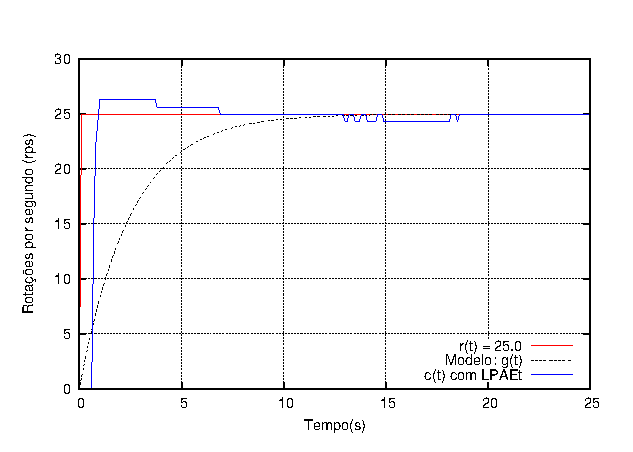
\includegraphics[scale=1.6]{./imagens/LPAEt-gct100.eps}
%\label{fig:acaoLPAEtgct100}

%{\small Fonte: Próprio autor}
%\end{figure}
%%%%%%%%%%%%%%%%%%%%%%%%%%%%%%%%%%%%%%%%%%%%%%%%%%





%######################################
%\begin{comment}


%\begin{figure}[!h]
%\centering
%\caption{Representação da região ativa no reticulado da LPA$E\tau$}
%\begin{tikzpicture}[scale=0.80]
%\tikzset{ >=latex, inner sep=0pt, outer sep=0pt,  }

%%\draw [lightgray, dashed](0,0) grid (10,10);

%\node [fill=black, circle] (V) at (9,5) {:};
%\node [fill=black, circle] (F) at (1,5) {:};
%\node [fill=black, circle] (T) at (5,9) {:};
%\node [fill=black, circle] (L) at (5,1) {:};

%\draw [->, thick] (V)   -- (10,5);
%\draw [    thick] (0,5) -- (F);
%\draw [->, thick] (T)   -- (5,10);
%\draw [    thick] (5,0) -- (L);

%\draw [thick] (V) -- (T);
%\draw [thick] (T) -- (F);
%\draw [thick] (F) -- (L);
%\draw [thick] (L) -- (V);

%\draw[thick] (SW) rectangle (NE);
%\fill[nearly transparent] (SW) rectangle (NE);

%\node at (10,4.5) {$G_{ce}$};
%\node at (5.5,10) {$G_{in}$};

%\node at (4.5,9.2) {$+1$};
%\node at (9.0,5.5) {$+1$};
%\node at (5.5,1.0) {$-1$};
%\node at (1.0,4.5) {$-1$};

%\node at (9.0,4.5) {V};
%\node at (1.0,5.5) {F};
%\node at (5.5,9.2) {$\top$};
%\node at (4.5,1.0) {$\bot$};

%\draw [fill, red,nearly transparent] (1.0,5.0) -- (1.5,5.5) -- (1.5,4.5) -- (1.0,5.0);
%\draw [fill, purple, nearly transparent] (1.5,5.5) -- (5.0,9.0) -- (5.2,8.8) -- (1.5,5.5);
%\draw [fill, blue, nearly transparent] (5.0,1.0) -- (8.0,4.0) -- (2.0,4.0) -- (5.0,1.0);
%\draw [fill, green, nearly transparent] (5.2,8.8) -- (2.1,6.0) -- (8.0,6.0) -- (5.2,8.8);

%\draw [fill, gray, nearly transparent] (4.0,6.0) -- (4.0,4.0)-- (6.0,4.0) -- (6.0,6.0) -- (4.0,6.0);


%\draw [dashed, purple] (5.2,8.8) -- (1.5,5.5);
%\draw [thick] (5.0,9.0) -- (1.0,5.0);
%\draw [gray,thick] (V) -- (F);


%\node at (5.0,7.0) {1};
%\node at (3.0,5.0) {$\mu_0 + \delta_0$};
%\node at (5.0,5.0) {$\mu_0 + \delta_1$};
%\node at (7.0,5.0) {$\mu_0 + \delta_n$};
%\node at (5.0,3.0) {0};

%\end{tikzpicture}
%\label{fig:regiaoAtivaMuDeltaN}

%{\small Fonte: Próprio autor }
%\end{figure}


%\end{comment}
%######################################




%Caso o tempo de 1 segundo seja muito alto para um 
%determinado processo, 
%para as perturbações envolvidas no processo,
%o tempo pode ser alterado para gerar uma resposta 
%mais rápida ou mais lenta. 




%%%%%%%%%%%%%%%%%%%%%%%%%%%%%%%%%%%%%%%%%%%%%%%%%%%%%%%%%%%%
%%%%%%%%%%%%%%%%%%%%%%%%%%%%%%%%%%%%%%%%%%%%%%%%%%%%%%%%%%%%


%\section{Diagrama PEREIRA-LEÃO}

%A LPA$E\tau$ pode estabelecer uma relação de semelhança com parâmetros
%típicos em automação e controle,
%de modo que podem ser facilmente interpretados e correlacionadas com
%variáveis manipulada e controlada, valores desejados e de sensores,
%bem como não linearidades, zona morta, saturação e histerese.



%%%%%%%%%%%%%%%%%%%%%%%%%%%%%%%%%%%%%%%%%%%%%% Fig
%\begin{figure}[!h]%%%%%%%%%%%%%%%%%%%%%%%%%%%%%%%%
%\centering
%\caption{Representação da LPA$E\tau$ no Diagrama Pereira-Leão}
%\begin{tikzpicture}[scale=0.70]
%\tikzset{ >=latex, inner sep=0pt, outer sep=0pt,  }

%\draw [lightgray, dashed](0,0) grid (10,10);

%\node [fill=black, circle] (V) at (9,5) {:};
%\node [fill=black, circle] (F) at (1,5) {:};
%\node [fill=black, circle] (T) at (5,9) {:};
%\node [fill=black, circle] (L) at (5,1) {:};

%\draw [->, thick] (V)   -- (10,5);
%\draw [    thick] (0,5) -- (F);
%\draw [->, thick] (T)   -- (5,10);
%\draw [    thick] (5,0) -- (L);

%\draw [thick] (V) -- (T);
%\draw [thick] (T) -- (F);
%\draw [thick] (F) -- (L);
%\draw [thick] (L) -- (V);

%\node at (10,4.5) {$G_{c}$};
%\node at (5.5,10) {$G_{i}$};

%\node at (4.5,9.2) {$+1$};
%\node at (9.0,5.5) {$+1$};
%\node at (5.5,1.0) {$-1$};
%\node at (1.0,4.5) {$-1$};

%\node at (9.0,4.5) {V};
%\node at (1.0,5.5) {F};
%\node at (5.5,9.2) {$\top$};
%\node at (4.5,1.0) {$\bot$};


%\draw [fill, purple,nearly transparent] (9.0,5.0) -- (8.5,5.5) -- (8.5,4.5) -- (9.0,5.0);
%\node at (10.0,7.5) {Região de};
%\node at (10.0,6.5) {Verdade};
%\draw [->, thick] (9.5,6.0) -- (8.70,5.20);

%\draw [fill, red,nearly transparent] (1.0,5.0) -- (1.5,5.5) -- (1.5,4.5) -- (1.0,5.0);
%\node at (0.0,3.5) {Região de};
%\node at (0.0,2.5) {Falsidade};
%\draw [->, thick] (0.5,4.0) -- (1.30,4.80);

%\draw [fill, green,nearly transparent] (1.5,5.5)--(2,6)--(8,6)--(8.5,5.5)--(8.5,4.5)--(8,4)--(2,4)--(1.5,4.5) -- (1.5,5.5);
%\node at (5.0,5.5) {Região de};
%\node at (5.0,4.5) {Trivialidade Admitida};



%\node at (0.0,9.5) {Região de Incerteza};
%\node at (0.0,8.5) {Máxima Positiva};
%\draw [->, thick] (2.5,8.0) -- (4.0,7.50);

%\node at (10.0,2.5) {Região de};
%\node at (10.0,1.5) {Incerteza Máxima Negativa};
%\draw [->, thick] (8.0,2.5) -- (6.00,3.00);

%\draw [fill, purple, nearly transparent] (1.5,5.5) -- (5.0,9.0) -- (5.2,8.8) -- (1.5,5.5);
%\draw [fill, blue, nearly transparent] (5.0,1.0) -- (8.5,4.5) -- (1.5,4.5) -- (5.0,1.0);
%\draw [fill, green, nearly transparent] (5.2,8.8) -- (2.1,6.0) -- (8.0,6.0) -- (5.2,8.8);

%\draw [thick] (5.0,9.0) -- (1.0,5.0);

%\node at (5.0,7.0) {1};
%\node at (5.0,5.0) {$\mu_0 + \delta$};
%\node at (5.0,3.0) {0};

%\draw [dashed, gray] (2.5,6.0) -- (2.5,4.5);
%\draw [dashed, gray] (3.5,6.0) -- (3.5,4.5);
%\draw [dashed, gray] (6.5,6.0) -- (6.5,4.5);
%\draw [dashed, gray] (7.5,6.0) -- (7.5,4.5);
%\draw [dashed, lightgray] (4.5,6.0) -- (4.5,4.5);
%\draw [dashed, lightgray] (5.5,6.0) -- (5.5,4.5);

%\end{tikzpicture}
%\label{fig:diagramaPereiraLeao}

%{\small Fonte: Próprio autor }
%\end{figure}
%%%%%%%%%%%%%%%%%%%%%%%%%%%%%%%%%%%%%%%%%%%%%%%%%%




%A aplicação da LPA$E\tau$ conforme estudada e implementada neste trabalho requer como
%proposição a correspondência direta à variável manipulada em seu valor máximo.
%Este valor máximo deve corresponder a condição verdade do diagrama.
%Assim, a proposição é verdadeira quando o máximo da variável manipulada é alcançada.

%Toda proposição apresenta duas anotações,
%sendo o grau de evidência favorável correspondente ao valor de referência do sistema, ou seja,
%ao valor desejado, $\mu$, enquanto que o grau de evidência contrária corresponde ao
%complemento do sinal do sensor, $\lambda$, desta forma,
%quando o sensor apresenta valor máximo, $\lambda = 0$, de maneira oposta,
%quando o sensor apresenta valor mínimo, $\lambda = 1$.

%O ponto gerado pela combinação $(\mu,\lambda)$ ao estar contido respectivamente em $(0,1)$,
%corresponde ao mínimo da variável controlada,
%enquanto que para a combinação extrema $(1,0)$ corresponde ao máximo da variável controlada.

%A primeira etapa de implementação do controlador utilizando LPA$E\tau$
%conforme apresentada neste trabalho,
%deve-se setar o máximo da variável manipulada com o máximo valor apresentado pelo sensor,
%de forma análoga a uma sistema em malha aberta, em que o máximo da referência produz o máximo
%valor da variável controlada.

%Para a condição em que o valor desejado e o sensor apresentam igualdade,
%o Grau de Incerteza é nulo, e o sistema não apresenta erro. Isso ocorre sempre que a
%anotação produzir um ponto sobre a reta do Grau de Certeza. Para uma variação dentro
%dos parâmetros admissíveis, a região correspondente, situada no entorno da linha de Grau de Certeza,
%próximo ao zero tanto quanto o sistema admitir, 
%recebe o nome de Região de Trivialidade Admitida. 


%A região que apresenta um Grau de Incerteza elevado recebe o nome de
%Região de Incerteza Máxima Positiva,
%e para o sistema estudado corresponde a condição em que a variável controlada está muito abaixo
%do valor desejado, assim, elevando a variável manipulada ao seu valor máximo, afim de anular o erro.

%A região que apresenta o Grau de de Incerteza mais baixo, recebe o nome de
%Região de Incerteza Máxima Negativa,
%o que corresponde à condição em que a variável controlada apresenta valor bem acima do valor desejado,
%produzindo um valor nulo na variável manipulada, situação tida como adequada para a situação aqui
%vista, e deve ser avaliada para cada situação em que o controlador venha ser utilizado.

%O conceito de zona morta pode ser representado pela região de falsidade,
%pois localiza-se em uma região em que a variável desejada apresenta um valor em que o sistema físico
%não reage ao estímulo, tendo um limiar em que a inércia de partida é vencida e o
%sistema se coloca em movimento, no caso do motor acoplado a uma carga.

%Em automação e controle, a zona morta é um conceito bem comum, assim como a saturação,
%que no diagrama Pereira-Leão pode ser apresentada na região de verdade, porém,
%ao ajustar os parâmetros,
%para o máximo da variável manipulada equivalente a máxima resposta do sistema,
%a saturação não ocorre, ou fica restrita a condição de verdade.




%A condição de falsidade é o Valor mínimo da variável controlada;
%O Grau de evidência favorável( $\mu$ ) como valor desejado, ou setpoint;
%O grau de evidência desfavorável ( $\lambda$ ) como valor do sensor da variável controlada;
%A região de falsidade é caracterizada como zona morta;
%A região de verdade é caracterizada como saturação;
%A trivialidade(incerteza) admitida corresponde a histerese.






%%%%%%%%%%%%%%%%%%%%%%%%%%%%%%%%%%%%%%%%%%%%%% Fig
%\begin{figure}[!h]%%%%%%%%%%%%%%%%%%%%%%%%%%%%%%%%
%\centering
%\caption{Representação da LPA$E\tau$ no Diagrama Pereira-Leão}
%\begin{tikzpicture}[scale=0.70]
%\tikzset{ >=latex, inner sep=0pt, outer sep=0pt,  }

%\draw [lightgray, dashed](0,0) grid (10,10);

%\node [fill=black, circle] (V) at (9,5) {:};
%\node [fill=black, circle] (F) at (1,5) {:};
%\node [fill=black, circle] (T) at (5,9) {:};
%\node [fill=black, circle] (L) at (5,1) {:};

%\draw [->, thick] (V)   -- (10,5);
%\draw [    thick] (0,5) -- (F);
%\draw [->, thick] (T)   -- (5,10);
%\draw [    thick] (5,0) -- (L);

%\draw [thick] (V) -- (T);
%\draw [thick] (T) -- (F);
%\draw [thick] (F) -- (L);
%\draw [thick] (L) -- (V);

%\node at (10,4.5) {$G_{c}$};
%\node at (5.5,10) {$G_{ct}$};

%\node at (4.5,9.2) {$+1$};
%\node at (9.0,5.5) {$+1$};
%\node at (5.5,1.0) {$-1$};
%\node at (1.0,4.5) {$-1$};

%\node at (9.0,4.5) {V};
%\node at (1.0,5.5) {F};
%\node at (5.5,9.2) {$\top$};
%\node at (4.5,1.0) {$\bot$};

%\draw [fill, red,nearly transparent] (1.0,5.0) -- (1.5,5.5) -- (1.5,4.5) -- (1.0,5.0);
%\draw [fill, purple, nearly transparent] (1.5,5.5) -- (5.0,9.0) -- (5.2,8.8) -- (1.5,5.5);
%\draw [fill, blue, nearly transparent] (5.0,1.0) -- (8.5,4.5) -- (1.5,4.5) -- (5.0,1.0);
%\draw [fill, green, nearly transparent] (5.2,8.8) -- (2.1,6.0) -- (8.0,6.0) -- (5.2,8.8);

%\draw [thick] (5.0,9.0) -- (1.0,5.0);

%\node at (5.0,7.0) {1};
%\node at (5.0,5.0) {$\mu_0 + \delta$};
%\node at (5.0,3.0) {0};

%\draw [dashed, gray] (2.5,6.0) -- (2.5,4.5);
%\draw [dashed, gray] (3.5,6.0) -- (3.5,4.5);
%\draw [dashed, gray] (6.5,6.0) -- (6.5,4.5);
%\draw [dashed, gray] (7.5,6.0) -- (7.5,4.5);
%\draw [dashed, lightgray] (4.5,6.0) -- (4.5,4.5);
%\draw [dashed, lightgray] (5.5,6.0) -- (5.5,4.5);

%\end{tikzpicture}
%\label{fig:diagramaPereiraLeao}

%{\small Fonte: Próprio autor }
%\end{figure}
%%%%%%%%%%%%%%%%%%%%%%%%%%%%%%%%%%%%%%%%%%%%%%%%%%




\chapter[Materiais e Métodos]{4. Materiais e Métodos}
Para o desenvolvimento deste trabalho foram dadas prioridade e
preferência para a utilização de um sistema embarcado de núcleo ARM,
com o intúito de desenvolver as capacidades de operar tal tecnologia
de processamento, trabalhando com sistema um eletrônico simples de fácil acesso mas que atenda as necessidades do projeto, bem como a utilização de ferramentas de uso livre.

Como metodologia foi adotado o procedimento de comparação de
resultados gerados entre uma técnica de controle bem estabalecida,
com uma lógica clássica utilizando um controlador
Proporcional+Integral (PI), e um controlador proposto
utilizando a LPA$E\tau$. 







\section{Materiais}

O protótipo físico foi constuído baseado em um microcontrolador da
família Texas Instruments, modelo $Tiva^{TM}$ TM4C123GH6PM, drive para
acionamento do tipo \emph{Pulse Width Modulation}(PWM) do motor com
circuito integrado de tecnologia CMOS (IRF540), motor de corrente
contínua acoplado a um disco compacto(CD), com uma etiqueta,
Figura \ref{fig:discoSensor}, para acionar o sensor óptico e servir de
indicador para contagem de giros do motor.
Fonte de alimentação chaveada de 12V 10W.
A maior parte do sistema pode ser visto na Figura \ref{fig:discoSensorGeral} .


\begin{figure}[!htb]
\center
\caption{Visão geral do sistema }
\subfloat[]{
	\label{fig:discoSensor}
	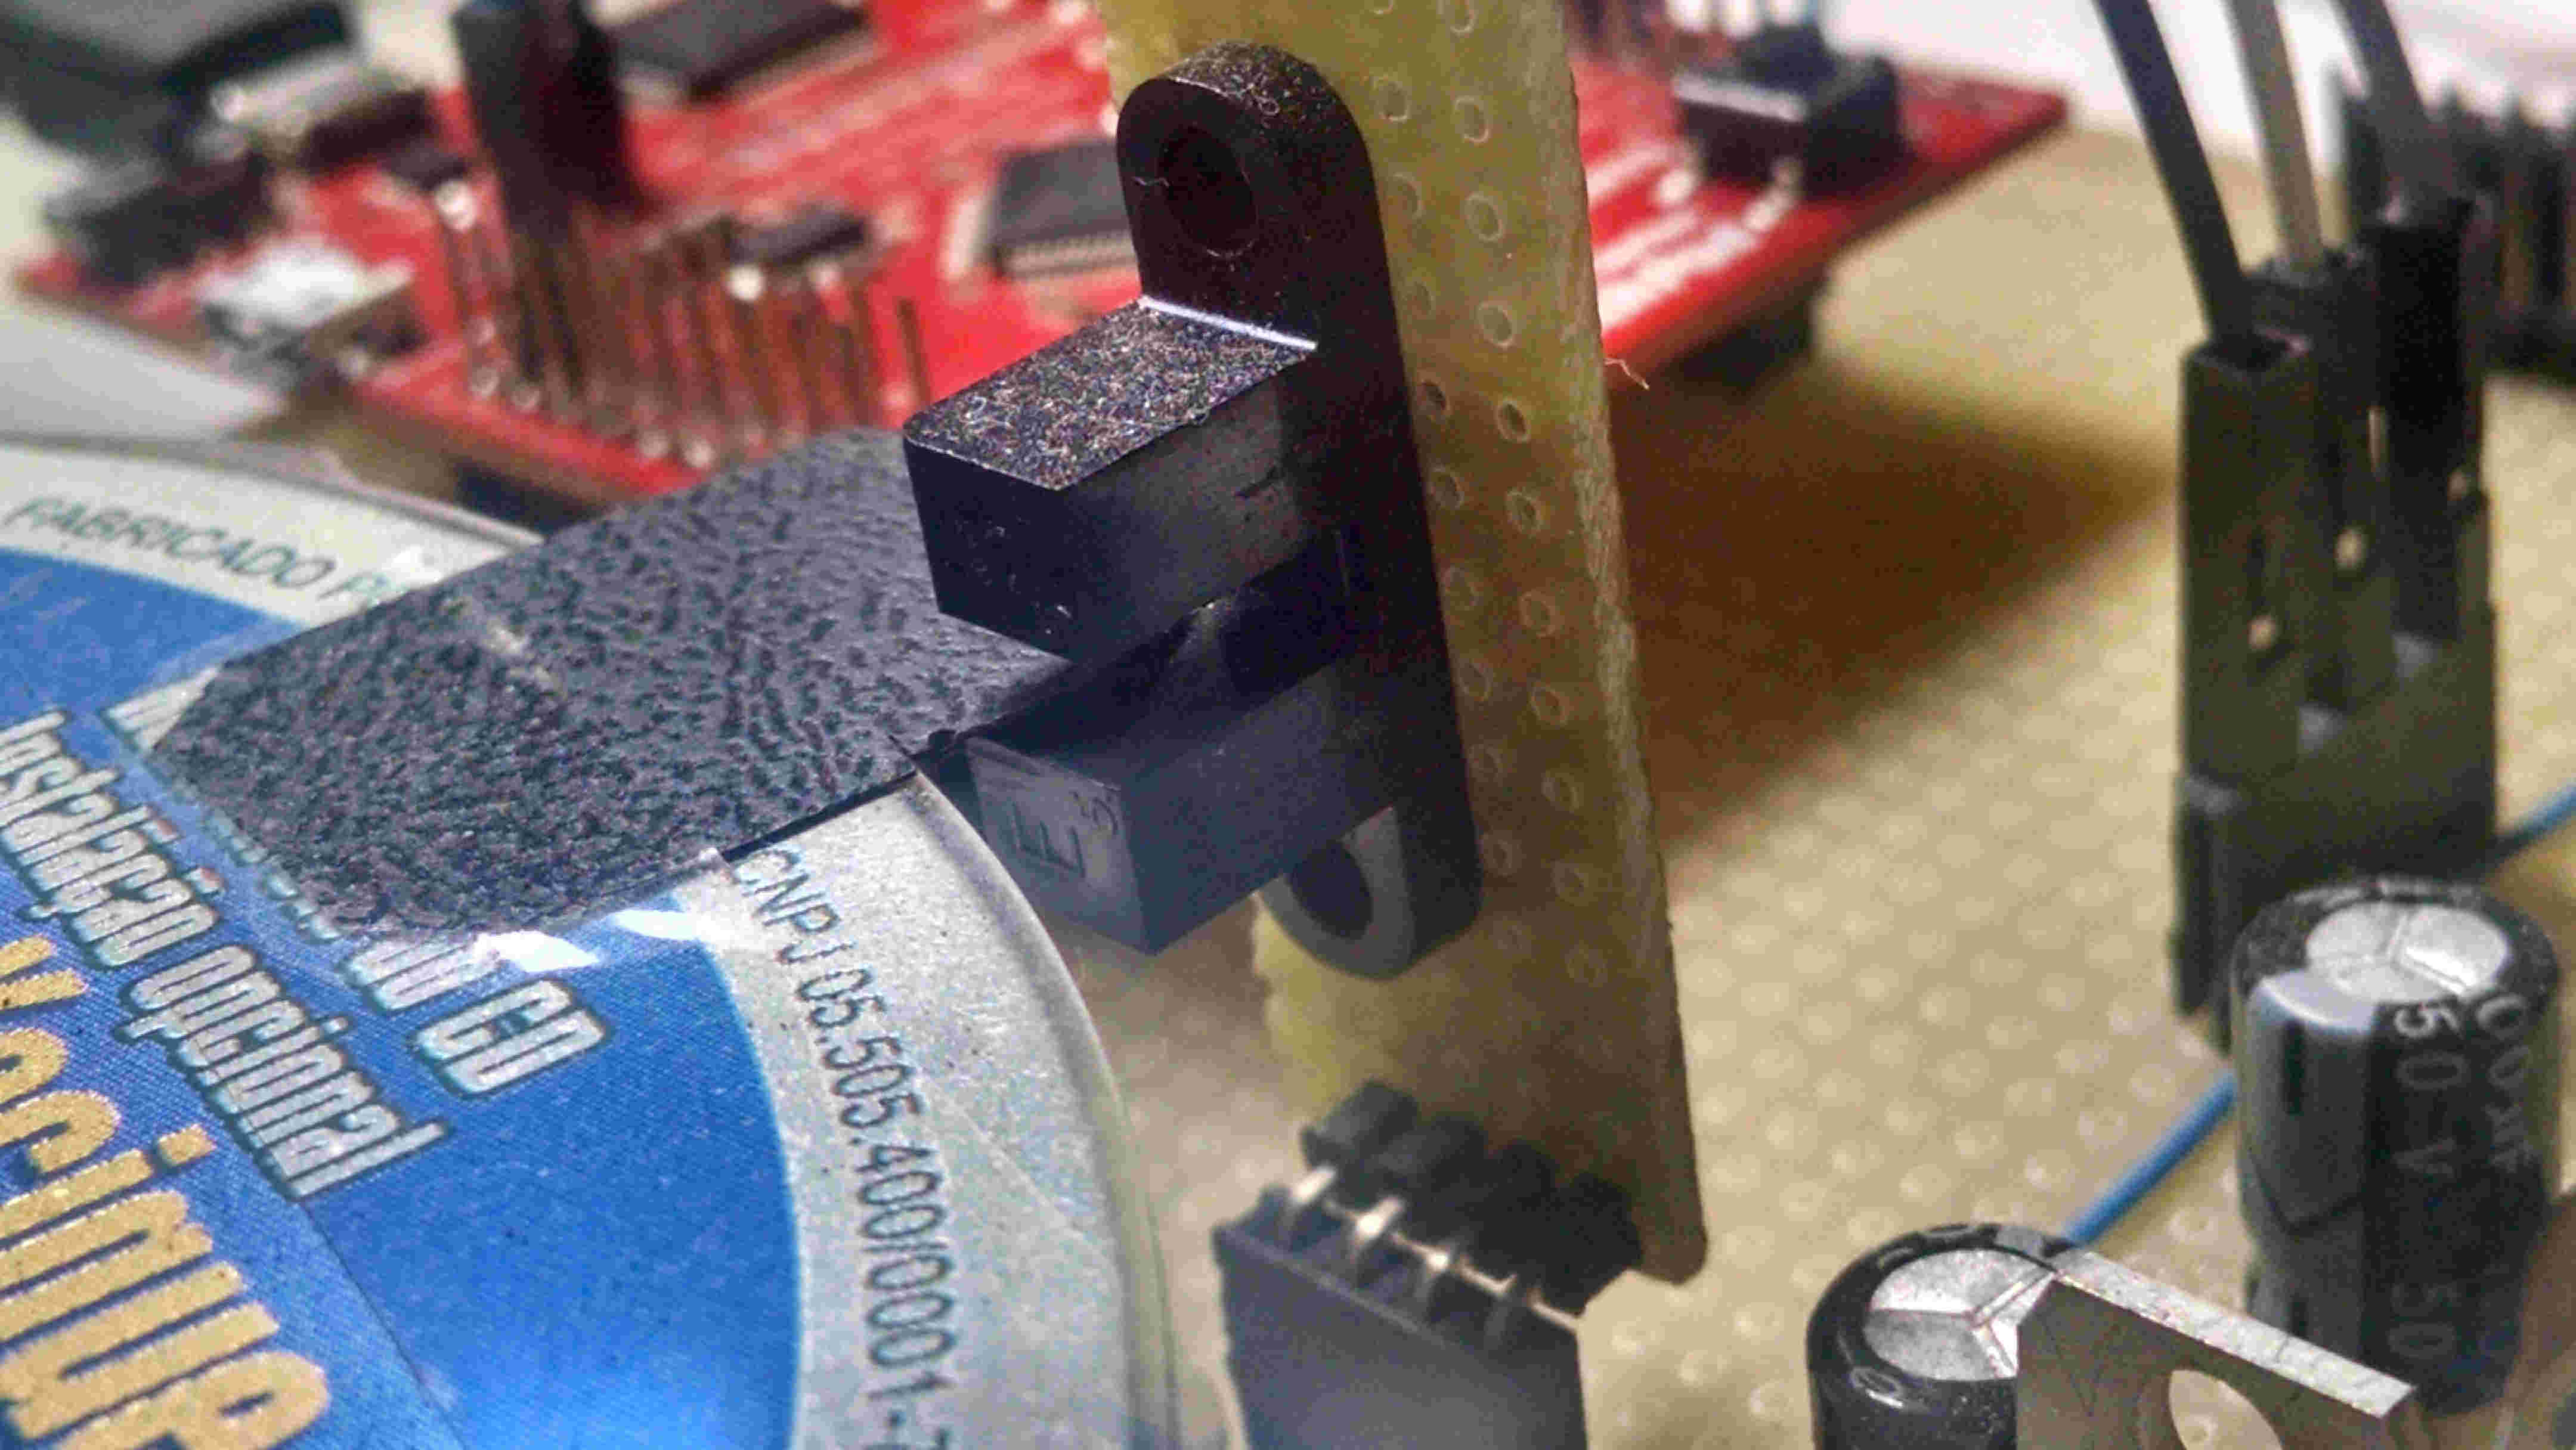
\includegraphics[scale=0.07, angle=0, clip=true, trim=300 200 1200 200]{./imagens/discoSensor.jpg}
	}
\subfloat[]{ 
	\label{fig:discoSensorGeral} 
	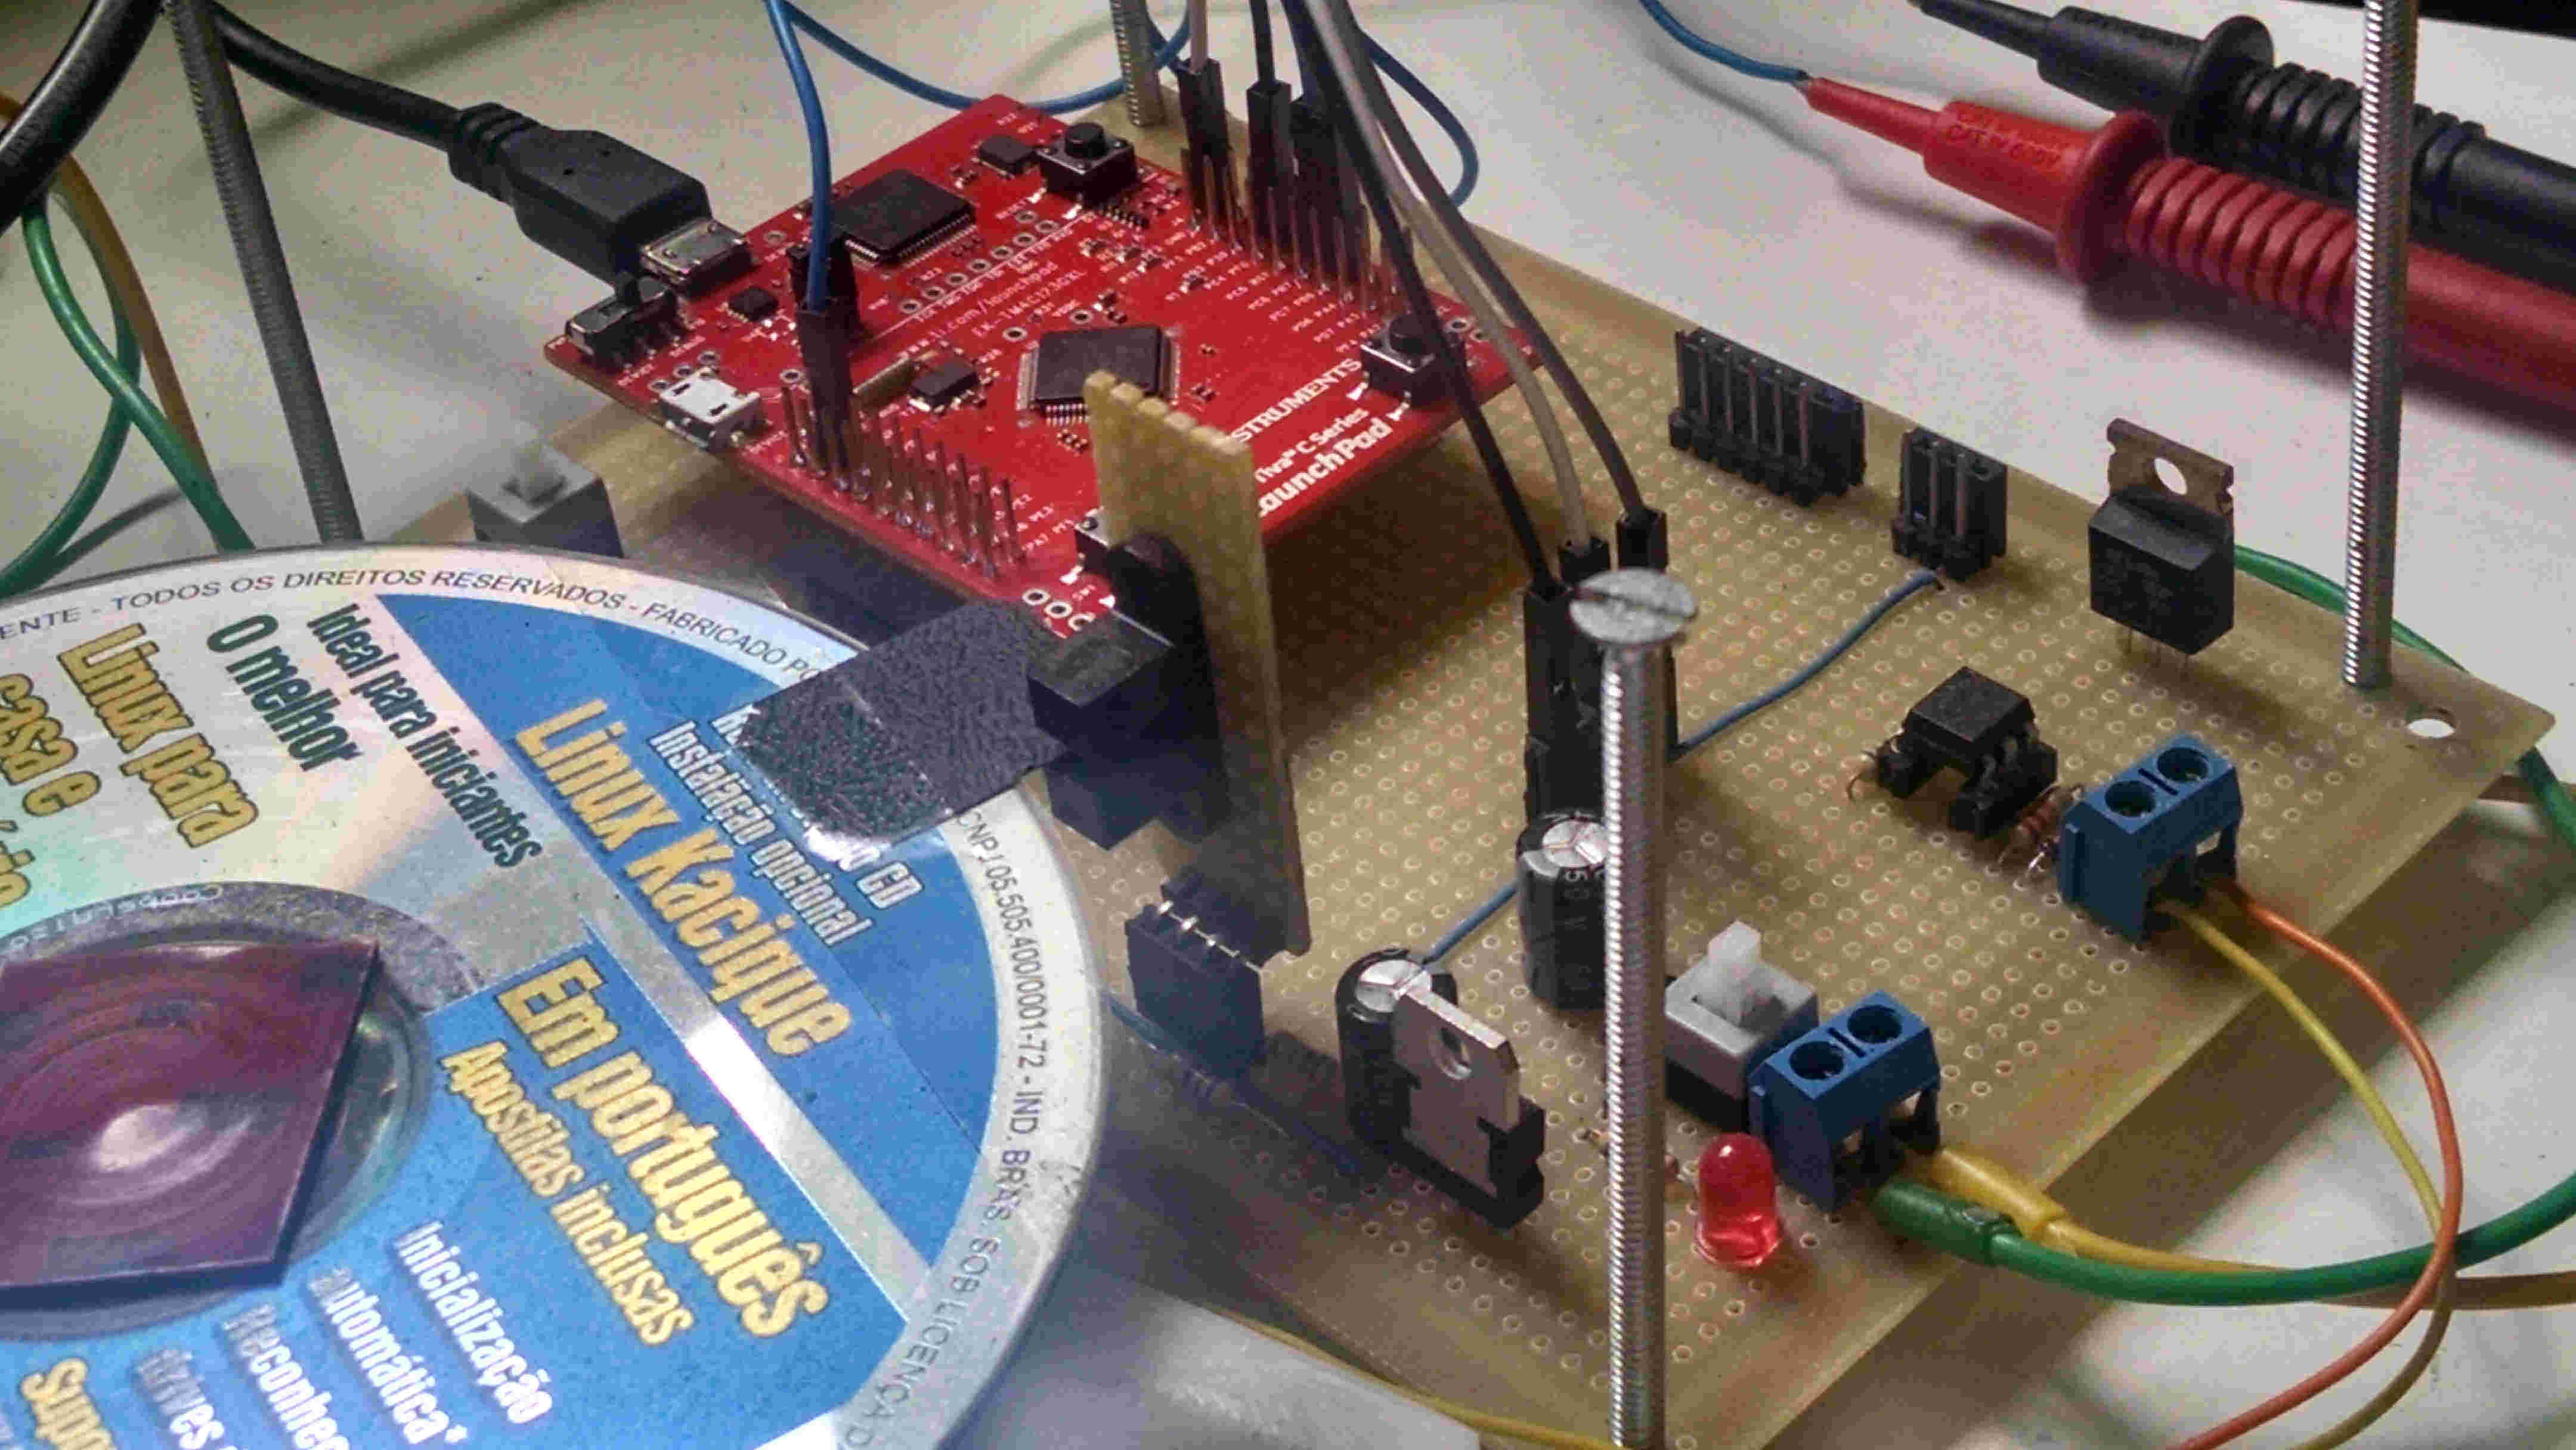
\includegraphics[scale=0.07, angle=0, clip=true, trim=300 200 400 200]{./imagens/discoSensorGeral.jpg} 
	}

{\small Figure: Próprio autor}
\end{figure}

As ferramentas de software utilizadas foram em sua totalidade de uso
livre ou de código aberto, sendo eles:

\begin{itemize}
\item Sistema Operacional GNU/Linux Debian 8(Jessie);
\item GNOME Shell;
\item Editores de texto e códigos fonte VIM e Emacs;
\item Compilador GCC para ARM (arm-none-eabi-gcc);
\item GNU Make;
\item Processador de texto \LaTeX - pdfTEX; 
\item Pacotes geradores de figuras TikZ, PGF e GNU pic(Groff);
\item Gerador de gráficos GNUPlot;
\item Teminal de comunicação Minicom;
\item Gravador para microcontrolador ARM LM4Flash.
\end{itemize}










\section{ Métodos }

Os métodos utilizados buscam mostrar como implementar e testar o
sistema de controle proposto, possibilitando uma posterior replicação
dos ensaios utilizados e análise da forma como o sistema foi
construído e testado.

%!@# rever frase completa
%Os métodos utilizados para a verificação do objetivo do projeto devem verificar quão próximo o resultado obtido empiricamente foi do objetivo esperado, de modo que as expectativas referentes aos objetivos propostos sejam atendidos ou sua 'negação' seja devidamente esclarecidas. 

Basicamente, são realizadas as seguintes etapas:

\begin{itemize}
\item Levantamento de um modelo matemático do sistema protótipo utilizado;
\item Verificação da qualidade desse modelo, com erro percentual médio
  menor do que 5\%, considerando um sistema não crítico. Se o erro
  percentual médio for maior do que os 5\%, retornar ao passo anterior e
  melhorar o modelo;
\item Definição dos requisitos de desempenho do sistema;
\item Realizar o controle utilizando um controlador PI;
\item Realizar o controle utilizando um controlador LPA$E\tau$;
\end{itemize}

\nomenclature{$PI$}{Proporcional-Integral}



\subsection{ Obtenção de um modelo matemático do processo }

A obtenção do modelo matemático do processo,
apresentada no anexo B, consiste em equacionar
regras matemáticas a partir da física básica do sistema,
de modo a obter uma função,
contemplando as as principais variáveis do sistema,
e que ajustadas adequadamente,
possam produzir um resultado semelhante ao comportamento do sistema
original, resultado empírico de funcionamento.



\subsection{ Qualidade do modelo }

Garantir uma boa qualidade ao modelo é importante para que se possa
utilizá-lo para calcular os parametros dos controladores.

A qualidade do modelo é relativa ao erro aceitável para o sistema estudado. Para o modelo obtido neste estudo foi aplicada o cálculo de Erro Relativo Percentual, e foram feitas análises em trechos diferentes em função da não linearidade inicial apresentada pelo comportamento do motor da planta em estudo.


A equação para o cálculo de Erro Relativo Percentual é:

\begin{equation}
 \% erro = \frac{| \text{\emph{valor real}} -\text{\emph{valor calculado}} |}{\text{\emph{valor real}}} x 100
\end{equation}

Realizando a somatória para o cálculo de erro médio com todas as
amostras a serem aquisitadas: 

\begin{equation}
 \% erro = \frac{100}{N} . \sum_{n = inicial}^{n = final} {\frac{| \text{\emph{r[n]}} -\text{\emph{c[n]}} |}{\text{\emph{r[n]}}} } 
\end{equation}


Onde:

\setlength{\parindent}{2cm}
r : valor real, empírico; 

c : valor calculado;

n : número da amostra aquisitada;

N : número total de amostras.




\subsection{ Requisitos de desempenho do sistema }

Os principais e mais comuns requisitos de desempenho dos sistemas são:

\begin{itemize}

\item Velocidade de resposta: A constante de tempo $\tau$ é a medida
  de tempo em que um sistema de primeira ordem alcança os $63\%$ do
  sinal máximo desejado, assumindo que para a estabilidade o sistema
  precisa de um tempo de cinco vezes o tempo do $\tau$. Assim, é
  definida como velocidade de resposta desejada uma estabilidade
  equivalente a duas vezes o  $\tau$, reduzindo a $\frac{2}{5}$ do valor
  inicial. 
%\item Velocidade de resposta: A Figura \ref{fig:acaoMalhaAberTau} mostra que para a constante de tempo $\tau$, foi registrado um intevalo de 2,5 segundos, assim, a estabilidade é alcançada em torno de 12,5 segundos, assumindo a partir daí o regime de estabilidade.
%Como requisito de desempenho é estipulada uma redução do tempo de resposta para $\frac{1}{2}$ do valor inicial, com o novo $\tau$ assimindo o valor máximo de 1,25 segundos.

\item Sobressinal: Para muitos sistemas ter um sobressinal elevado é algo completamente indesejado, outros permitem alguma oscilação, no caso aqui estudado é definido que o sobressinal aceitável é de no máximo $10\%$ do valor desejado.
  
\item Erro de regime estacionário: é a exatidão da resposta do sistema em relação ao valor desejado, assume-se um valor aceitável para o sistema, nesse caso não crítico, de $5\%$.
\end{itemize}



\subsection{ Ensaio com o controlador Liga/Desliga }

O controlador Liga/Desliga é o de mais fácil implementação, porém não
apresenta um controle muito eficiente. Consiste em acionar a carga
com 100$\%$ da alimentação até que a saída alcance o valor desejado,
desligando-a e retornando a ligá-la quando estiver abaixo do valor
desejado, ficando num ciclo de liga-desliga. 



\subsection{ Ensaio com o controlador PI }

A ação de controle Proporcional+Integral (PI) é adequada ao sistema
proposto utilizado neste estudo.

A Equação \ref{eq:metodoPI} descreve o controlador PI a ser implementado.

\begin{equation}
  u(t) = kp.e(t) + ki \int_{0}^{\infty} e(t) dt
\label{eq:metodoPI}  
\end{equation}


\subsection{ Ensaio com o controlador LPA$E\tau$ }

O controlador LPA$E\tau$ a ser implementado é mostrado na Figura 
\ref{fig:metodoControleLPAEt}, de modo que o $\mu_0 + \delta$ sejam
ajustados de acordo com a Tabela \ref{tab:correcaoDelta}, conforme
exposto no respectivo capítulo.

%%%%%%%%%%%%%%%%%%%%%%%%%%%%%%%%%%%%%%%%%%%%%% Fig
\begin{figure}[!h]%%%%%%%%%%%%%%%%%%%%%%%%%%%%%%%%
\centering
\caption{Representação do reticulado da LPA$E\tau$ para o controlador}
\begin{tikzpicture}[scale=0.80]
\tikzset{ >=latex, inner sep=0pt, outer sep=0pt,  }

%\draw [lightgray, dashed](0,0) grid (10,10);

\node [fill=black, circle] (V) at (9,5) {:};
\node [fill=black, circle] (F) at (1,5) {:};
\node [fill=black, circle] (T) at (5,9) {:};
\node [fill=black, circle] (L) at (5,1) {:};

\draw [->, thick] (V)   -- (10,5);
\draw [    thick] (0,5) -- (F);
\draw [->, thick] (T)   -- (5,10);
\draw [    thick] (5,0) -- (L);

\draw [thick] (V) -- (T);
\draw [thick] (T) -- (F);
\draw [thick] (F) -- (L);
\draw [thick] (L) -- (V);

\node at (10,4.5) {$G_{c}$};
\node at (5.5,10) {$G_{ct}$};

\node at (4.5,9.2) {$+1$};
\node at (9.0,5.5) {$+1$};
\node at (5.5,1.0) {$-1$};
\node at (1.0,4.5) {$-1$};

\node at (9.0,4.5) {V};
\node at (1.0,5.5) {F};
\node at (5.5,9.2) {$\top$};
\node at (4.5,1.0) {$\bot$};

\draw [fill, red,nearly transparent] (1.0,5.0) -- (1.5,5.5) -- (1.5,4.5) -- (1.0,5.0);
\draw [fill, purple, nearly transparent] (1.5,5.5) -- (5.0,9.0) -- (5.2,8.8) -- (1.5,5.5);
\draw [fill, blue, nearly transparent] (5.0,1.0) -- (8.5,4.5) -- (1.5,4.5) -- (5.0,1.0);
\draw [fill, green, nearly transparent] (5.2,8.8) -- (2.1,6.0) -- (8.0,6.0) -- (5.2,8.8);

\draw [thick] (5.0,9.0) -- (1.0,5.0);

\node at (5.0,7.0) {1};
\node at (5.0,5.0) {$\mu_0 + \delta$};
\node at (5.0,3.0) {0};

\draw [dashed, gray] (2.5,6.0) -- (2.5,4.5);
\draw [dashed, gray] (3.5,6.0) -- (3.5,4.5);
\draw [dashed, gray] (6.5,6.0) -- (6.5,4.5);
\draw [dashed, gray] (7.5,6.0) -- (7.5,4.5);
\draw [dashed, lightgray] (4.5,6.0) -- (4.5,4.5);
\draw [dashed, lightgray] (5.5,6.0) -- (5.5,4.5);

\end{tikzpicture}
\label{fig:metodoControleLPAEt}

{\small Fonte: Próprio autor }
\end{figure}
%%%%%%%%%%%%%%%%%%%%%%%%%%%%%%%%%%%%%%%%%%%%%%%%%%








\chapter[Resultados]{5. Resultados}
A obtenção do modelo matemático resulta em uma equação conforme segue.
Os detalhes do equacionamento podem ser acompanhados no Anexo B.
A Equação \ref{eq:resultadoModelo}, no formato canônico,  mostra a constante de tempo $\tau
= 2,5s$, para o sistema de primeira ordem utilizado neste estudo.  

\begin{equation}
  \frac{C(s)}{R(s)} = \frac{1}{\tau s+1} = \frac{1}{2,5 s+1}
\label{eq:resultadoModelo}
\end{equation}

Na Figura \ref{fig:resultadoft} pode ser visualisada a 
escala de tempo devidamente ajustada para um intervalo de mesmo
valor da constante de tempo $\tau$, facilitando a interpretação do
sinal aquisitado.

\begin{figure}[!htb]
\centering
\caption{Resultado gráfico do modelo matemático}
\center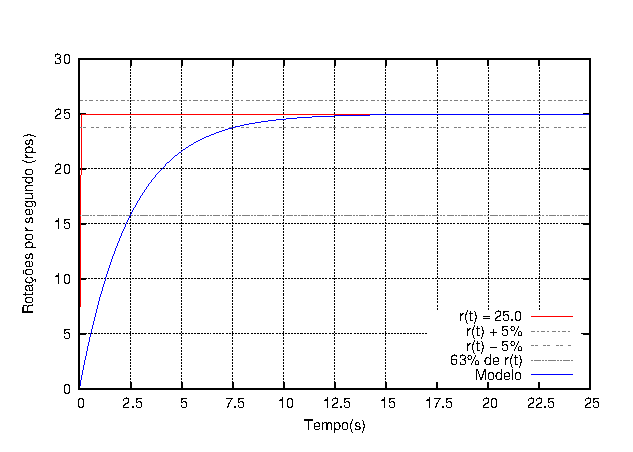
\includegraphics[scale=1.3]{./plot/ft.eps}

\label{fig:resultadoft}

{\small Fonte: Próprio autor}
\end{figure}



Ao aquisitar a curva de acionamento do sistema em malha aberta,
constuindo o gráfico das curvas aquisitada e calculada juntas  temos o
que é mostrado na Figura \ref{fig:resultadoMalhaAberta}:


\begin{figure}[!htb]
\centering
\caption{Comparação do modelo matemático com o comportamento empírico}
\center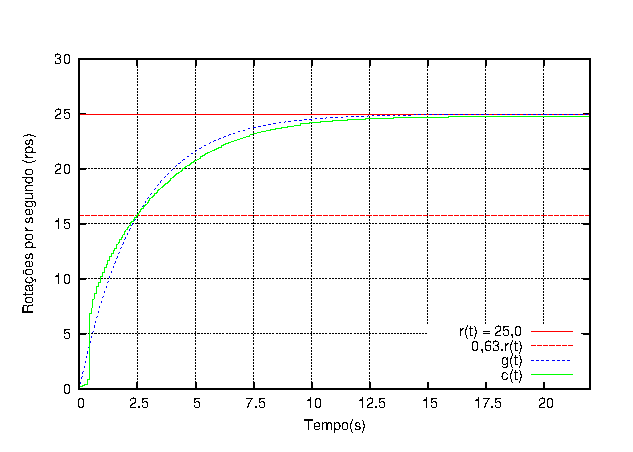
\includegraphics[scale=1.3]{./plot/acaoMalhaAbertaTau.eps}

\label{fig:resultadoMalhaAberta}

{\small Fonte: Próprio autor}
\end{figure}

Realizando a somatória para o cálculo de erro médio com todas as amostras aquisitadas: 

\begin{equation}
 \% erro = \frac{100}{N} . \sum_{n = 0,00}^{n=22,40} {\frac{| \text{\emph{r[n]}} -\text{\emph{c[n]}} |}{\text{\emph{r[n]}}} } 
\end{equation}


Onde:

\setlength{\parindent}{2cm}
r : valor real; 

c : valor calculado;

n : número da amostra aquisitada;

N : número total de amostras.

Obs.: As aquisições começaram com tempo inicial de 0,00 s até o tempo final de 22,40 segundos, com intervalo de 10 milisegundos entre aquisições, totalizando 2240 amostras.

\setlength{\parindent}{1cm}


Foi obtido um valor médio de 2,71\% de erro 
para o intervalo de aquisição de 50ms até os 22,40 s, 
que é o fim da aquisição, 
desconsiderando a região transitória não linear 
que ocorre nos instantes iniciais, 
mas que considera-se não relevante para a atual análise, 
inclusive pelo baixo valor de erro no restante do intervalo de comparação.


De forma mais detalhada, 
foram calculados os erros médios relativos para cada intervalo de 
tempo de um $\tau$, 
e pode-se notar, 
pela Tabela \ref{tab:resultadoErroModeloTau}, 
que o erro de estado estacionário, para o intervalo acima de 5 $\tau$, é menor do que 1\%. 


\begin{table}[h]
\centering
\caption{Erro Relativo Percentual para intervalos determinados por $\tau$ }
\label{tab:resultadoErroModeloTau}

\begin{tabular}{c|c}
\hline
Intervalo de amostras  &  erro médio relativo \\ \hline
\hline
%0 a 1 $\tau$ & 83,40 \% \\ \hline
1 a 2 $\tau$ &  3,16 \% \\ \hline
2 a 3 $\tau$ &  3,38 \% \\ \hline
3 a 4 $\tau$ &  2,00 \% \\ \hline
4 a 5 $\tau$ &  2,29 \% \\ \hline
$>$ 5 $\tau$ &  0,82 \% \\ \hline
\end{tabular}

{\vspace{0.2cm} \small Fonte: Próprio autor}
\end{table}

Desconsiderando a região transitória não linear 
que ocorre nos instantes iniciais do movimento do eixo do motor, 
o intervalo de maior erro é de 3,38\%, 
conforme mostrado na Tabela \ref{tab:resultadoErroModeloTau},
ressaltando ainda que no regime estacionário 
o erro é menor do que 1\%.
Assim, considera-se que o modelo utilizado é bom e representa razoavelmente bem o sistema físico real.

A Figura \ref{fig:resultadoAcaoPILPAEt} mostra de forma sobreposta os
resultados, em forma gráfica, para um sinal de referência do tipo
degrau e com valor em 25 rps, sendo acompanhado por linhas tracejadas
nos valores de tolerância de  $\pm 5\%$, bem como o comportamento da
planta em malha aberta, para que se possa ter uma melhor dimensão
do comportamente nos ensaios utilizando os controles PI e LPA$E\tau$ com diagrama Pereira-Leão.
A grade de apresentação do gráfico foi mantida com intervalo de 2,5s para o
período, mantendo cada unidade igual a um $\tau$. 





\begin{figure}[!htb]
\centering
\caption{Resultado dos controladores PI e LPA$E\tau$}
\center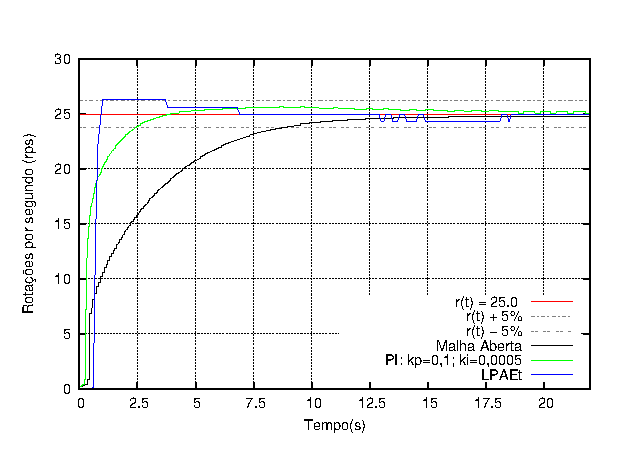
\includegraphics[scale=1.6]{./plot/resAcaoPI.eps}
\label{fig:resultadoAcaoPILPAEt}

{\small Fonte: Próprio autor}
\end{figure}









A resposta obtida para o sistema estudado pode ser vista na Figura \ref{fig:resultadoAcaoPILPAEt} onde podem ser destacados os seguintes pontos:

\begin{itemize}
\item No momento inicial, há um atraso de resposta devido à inércia do
  sistema físico, porém ao vencer esta condição inicial a velocidade
  de regime é alcançada rapidamente, em um tempo pouco menor do que $\frac{1}{2}$ do valor da constante de tempo $\tau$ do modelo do sistema.

\item O sobressinal apresentado alcança um valor ligeiramente acima da
  indicação superior de $5\%$ do valor de referência, metade do limite máximo aceitável de acordo com os requisitos de desempenho do sistema.

\item O sistema utilizando um controle PI entra em regime no tempo de
  2,5s, enquanto que para o controlador LPA$E\tau$ o regime é
  alcançado com um tempo de 3,75s, considerando que o sobressinal
  ligeiramente acima dos $5\%$ não é aceito para a janela do sistema
  em regime. Se tal valor for considerado e aceitável, o controlador
  LPA$E\tau$ entra em regima com um tempo de 1,75s aproximadamente.
Para o sistema em malha aberta o regime é alcançado com tempo de 8,75s. 

\end{itemize}


A Tabela \ref{tab:resultadoComparaErros}
mostra o erro médio relativo do
resultado dos dois controladores.
Em função do tempo de resposta
inicial, para esta tabela foi utilizado um intervalo de um segundo para gerar as amostras.

Um destaque pode ser dado aos dois primeiros intervalos de amostra,sendo que cada controlador obteve melhor desempenho em um deles.




\begin{table}[h]
\centering
\caption{Erro Médio Relativo Percentual }
\label{tab:resultadoComparaErros}


\begin{tabular}{c|c|c}
\hline
Intervalo de amostras  &  Controle PI &
Controle LPA$E\tau$ \\ \hline
\hline
 0 a  1 s & 50,57 \% &  75,68 \% \\ \hline
 1 a  2 s & 13,50 \% &  -5,20 \% \\ \hline
 2 a  3 s &  5,48 \% &  -5,20 \% \\ \hline
 3 a  4 s &  1,62 \% &  -4,64 \% \\ \hline
 4 a  5 s &  0,10 \% &  -2,40 \% \\ \hline
 5 a  6 s & -0,65 \% &  -2,40 \% \\ \hline
 6 a  7 s & -1,19 \% &  -2,16 \% \\ \hline
 7 a  8 s & -1,62 \% &   0,00 \% \\ \hline
 8 a  9 s & -1,78 \% &   0,00 \% \\ \hline
 9 a 10 s & -1,78 \% &   0,00 \% \\ \hline
10 a 11 s & -1,64 \% &   0,00 \% \\ \hline
11 a 12 s & -1,31 \% &   0,00 \% \\ \hline
12 a 13 s & -0,96 \% &   0,00 \% \\ \hline
13 a 14 s & -0,87 \% &   1,40 \% \\ \hline
14 a 15 s & -0,58 \% &   1,68 \% \\ \hline
15 a 16 s & -0,50 \% &   2,80 \% \\ \hline
16 a 17 s & -0,18 \% &   2,80 \% \\ \hline
17 a 18 s & -0,28 \% &   2,80 \% \\ \hline
18 a 19 s &  0,00 \% &   0,84 \% \\ \hline
19 a 20 s &  0,21 \% &   0,00 \% \\ \hline

\end{tabular}

{\vspace{0.2cm} \small Fonte: Próprio autor}
\end{table}




O primeiro intervalo de amostras (0 a 1s),
o controle PI obtem um resultado melhor,
pois apresenta um erro,
apesar de muito elevado,
muito menor do que o controlador LPA$E\tau$.
O segundo intervalo de amostras (1 a 2s),
pode-se notar que o erro está menor do que o
requisito de desempenho para este sistema
para o controlador LPA$E\tau$,
mas ainda não atingiu o mesmo limiar com
o controlador PI.  

O restante dos intervalos apresentam resultado satisfatório pois
apresentam-se dentro dos requisitos de desempenho do sistema, em ambos
os controles.













%\begin{figure}[!htb]
%\caption{Controle utilizando LPAE$\tau$}
%\center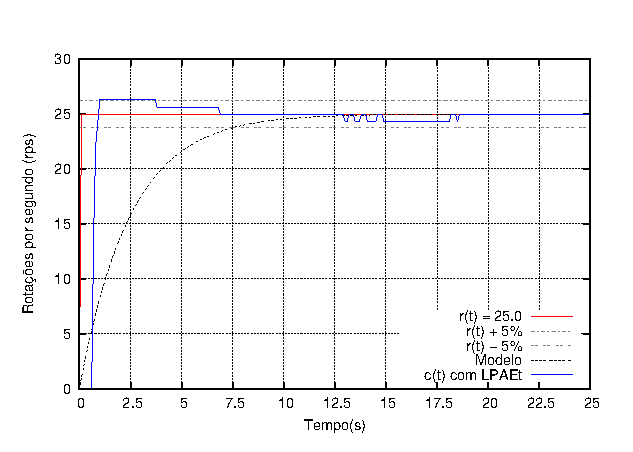
\includegraphics[scale=1.4]{./imagens/a3.eps}
%\label{fig:lpaet}

%{\small Fonte: Próprio autor}
%\end{figure}

%Todos os requisitos de desempenho do sistema foram atendidos, cumprindo com o objetivo inicial como pode-se ver na Figura \ref{fig:lpaet}. 





\section{Outros testes realizados}

Alguns testes foram realizados para validar a aplicação do $\delta$
(delta) na correção do controle na condição de regime.
Considerando que o intúito do presente trabalho não é gerar um
algorítmo de correção, mas que dentro da linha adotada houve a
necessidade de sua utilização. Cabendo a trabalhos futuros validar ou
refutar seu uso, bem como produzir formas de correção eficientes. 

A Figura \ref{fig:acaoLPAEtDelta} mostra a aquisição feita para
cinco(5) degraus de acionamento realizados sequencialmente.
Como pode-se ver, na resposta do primeiro degrau há um maior
sobressinal, sendo que este atenuado nos demais ciclos de acionamento,
em função de correção do $\delta$ do patamar em execução
correspondente a correção da velocidade desejada.

%%%%%%%%%%%%%%%%%%%%%%%%%%%%%%%%%%%%%%%%%%%%%% Fig
\begin{figure}[!htb]%%%%%%%%%%%%%%%%%%%%%%%%%%%%%%
\caption{Ação de controle utilizando LPA$E\tau$}
\vspace{-1cm}\center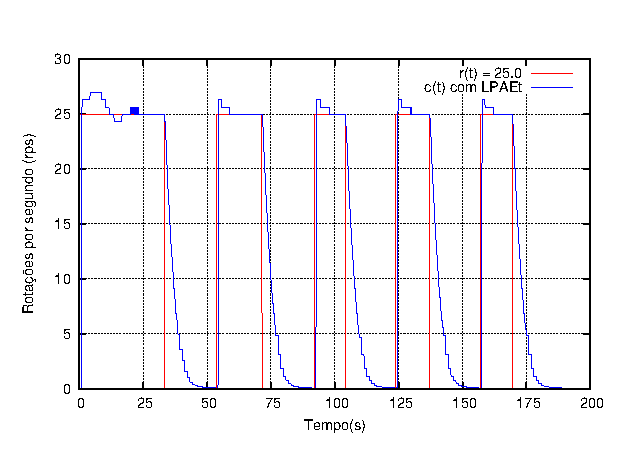
\includegraphics[scale=1.6]{./plot/LPAEt-delta.eps}
\label{fig:acaoLPAEtDelta}

{\small Fonte: Próprio autor}
\end{figure}
%%%%%%%%%%%%%%%%%%%%%%%%%%%%%%%%%%%%%%%%%%%%%%%%%%

Em outro teste, foram ajustandos os limiares,
e foi possível chegar ao resultado mostrado na Figura \ref{fig:LPAEterro}, 
onde pode-se comparar o resultado em dois momentos distintos,
no primeiro e no segundo ciclo,
comparativamente ao modelo gerado no Capítulo 3 deste trabalho.


%%%%%%%%%%%%%%%%%%%%%%%%%%%%%%%%%%%%%%%%%%%%%% Fig
\begin{figure}[!htb]%%%%%%%%%%%%%%%%%%%%%%%%%%%%%%
\caption{Erro na Ação de controle utilizando LPA$E\tau$}
\vspace{-1cm}\center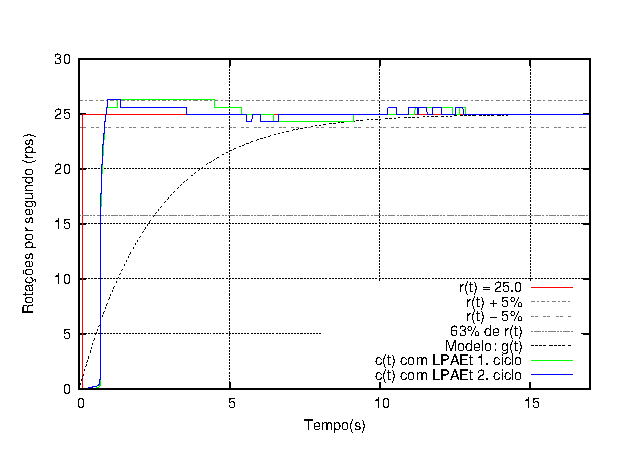
\includegraphics[scale=1.5]{./plot/LPAEt-erro.eps}
\label{fig:LPAEterro}

{\small Fonte: Próprio autor}
\end{figure}
%%%%%%%%%%%%%%%%%%%%%%%%%%%%%%%%%%%%%%%%%%%%%%%%%%

%A Figura \ref{fig:LPAEterro} mostra alguns parâmetros de 
%referência, como o valor de referência, 
%$r(t) = 25.0$ e linhas tracejadas indicando a 
%tolerância adotada como critério de desempenho de 
%$\pm $5\% além da curva do modelo do sistema.

O resultado obtido com o Controlador utilizando a 
LPA$E\tau$ proposta com o diagrama Pereira-Leão, é apresentada em dois sinais sobrepostos,
um para cada ciclo de operação, 
pois, no primeiro ciclo, a variável de correção $\delta$
ainda não foi ajustada, e a partir do segundo ciclo em diante, 
a resposta é mais rápida e mais acertiva pois já há um
valor de correção carregado, 
levando em consideração o ciclo anterior. 
Mesmo que não seja o mais adequado, 
deve ser o mais próximo do valor desejado, 
permitindo uma correção mais rápida, 
como se vê na resposta do segundo ciclo.


Pode ser destacada a redução do período em que o sistema atua
ligeiramente acima do limiar de $5\%$, consideravelmente reduzido.


Para evidenciar o ganho de performance, 
foi calculado o erro relativo percentual médio,
da mesma forma como foi realizado para obtenção do modelo
do sistema em estudo, 
apresentado neste capítulo.

A Tabela \ref{tab:ErroLPAEt} mostra
a comparação entre o primeiro e o segundo ciclo de acionamento do
sistema. Para cada ciclo foi feita a amostragem do sinal em um
intervalo que varia de 0,00s até 17,00s. A análise de cada um dos ciclos é
apresentada considerando a zona morta em uma das amostras e
desconsiderando-a em outra. Para ambos os tipos de intervalo, o erro médio
relativo cai no segundo ciclo, independente de considerar ou não a
zona morta. Mas ressalta-se que a zona morta causa um erro relativo
considerável à análise completa do sinal. Lembrando que o erro é
calculado em relação ao valor de referência $r(t)$. 
Como pode ser visto, há um ganho percentual de 
aproximadamento 1\% entre a atuação do primeiro 
para o segundo ciclo de acionamento. 



%%%%%%%%%%%%%%%%%%%%%%%%%%%%%%%%%%%%%%%%%%%%%% Tab
\begin{table}[h]%%%%%%%%%%%%%%%%%%%%%%%%%%%%%%%%%%
\centering
\caption{Erro Relativo Percentual do controlador LPA$E\tau$}
\label{tab:ErroLPAEt}

\begin{tabular}{c|c|c|c}
\hline
Ciclo de Atuação & Tipo de intervalo & Intervalo de amostras  &  erro médio relativo \\ \hline
\hline
1º & com zona morta & 0,00 a 17,00 s &  5,44 \% \\ \hline
1º & sem zona morta & 0,88 a 17,00 s &  1,90 \% \\ \hline
2º & com zona morta & 0,00 a 17,00 s &  4,41 \% \\ \hline
2º & sem zona morta & 0,88 a 17,00 s &  0,82 \% \\ \hline
\end{tabular}

{\vspace{0.2cm} \small Fonte: Próprio autor}
\end{table}
%%%%%%%%%%%%%%%%%%%%%%%%%%%%%%%%%%%%%%%%%%%%%%%%%%



%%%%%%%%%%%%%%%%%%%%%%%%%%%%%%%%%%%%%%%%%%%%%%%%%%
%%%%%%%%%%%%%%%%%%%%%%%%%%%%%%%%%%%%%%%%%%%%%%%%%%


\chapter[Conclusão]{6. Conclusão}
O presente trabalho apresentou uma
proposta ousada pela inovação na utilização da
Lógica Paraconsistente Anotada Evidencial $E\tau$
(LPA$E\tau$) aplicada em constrole de sistemas,
mesmo que de modo ainda inicial,
procurando conciliar
alguns conceitos e contornar outros.
Por se tratar de uma forma
até então não explorada,
pode-se perceber algumas possibilidades
tanto em configurações alternativas do
controlador como nas possibilidades de
que se apresentam como promissoras.

A nova proposta para realização do
controle dinâmico de sistema utilizando a
LPA$E\tau$,
através da configuração Pereira-Leão
para o controlador,
pôde ser verificada através da
aplicação de um método de validação
dessa nova proposta baseada em
comparação com uma implementação bem estabelecida,
aceita e utilizada pelo meio
acadêmico e industrial,
é destacadamente um passo de
considerável relevância na exploração de
novas aplicações da LPA$E\tau$.

Aplicação se mostrou bem sucedida mediante o objetivo e aos requisitos de desempenho do sistema apresentados, considerando satisfatória a aplicação da LPA$E\tau$ em sistema de controle através do controlador baseado no diagrama Pereira-Leão.

A compreensão da LPA$E\tau$ e
suas formas de aplicação,
a investigação das possibilidades e
áreas distintas de aplicação
contribuem para a ampliação do
seu conhecimento sob uma perspectiva
até então não explorada,
possibilitando o início de
uma linha de pesquisa
tendo como base o estudo da LPA$E\tau$
aplicada ao controle de sistemas e
evidenciar possibilidades de trabalhos futuros.



Os resultados obtidos neste trabalho são iniciais do ponto de vista de exploração da Lógica Paraconsistente Anotada Evidencial $E\tau$ utilizada para o controle dinâmico de sistemas, e apresenta-se como promissor o caminho associado à técnicas de sistemas adaptativos, inteligência artificial, para alteração de parâmetros de controle.


\section{Trabalhos futuros}

Como um dos principais resultados do presente trabalho está o apontamento de possíveis caminhos a serem trilhados futuramente, dando prosseguimento à linha de trabalho, ampliando os horizontes, sedimentando os conhecimentos aqui apresentados, corrigindo os posssíveis equívocos e aprofundando conceitos.

Como principais sugestões para trabalhos futuros são citados:

\begin{itemize}

\item Controle de sistemas não lineares: o presente trabalho, por se tratar de uma abordagem inicial, buscou uma aplicação em um sistemas mais simples, para validar os conceitos iniciais, reduzindo as possíveis fontes de complexidade e problemas;

\item Aplicar o controlador Pereira-Leão com a LPA$E\tau$ em um sistema de segunda ordem e avaliar as implicações, limitações e potenciais;
  
\item Controle de sistems críticos: aplicar a LPA$E\tau$ em sistemas cuja criticidade é mandatória, exigindo um processamento e tomada de decisão consistente, precisa e de resposta imediata;

\item Utilizar um sistema operacional de tempo real para gerenciar o comportamento do controlador, explorando o viés comportamental da implementação do controlador LPA$E\tau$ em um RTOS tanto \emph{soft} quanto \emph{hard}, com aplicações não críticas e críticas;

\nomenclature{$RTOS$}{$\emph{Real Time Operating Systems}$ - Sistema Operacional de Tempo Real}
  
\item Melhoria da geração do parâmetro $\delta$, utilizando um algorítmo adaptativo, inteligência artificial, ou alguma técnica que permita um melhor ajuste deste valor de correção.
  
\end{itemize}




%O processo de implementação do controlador utilizando a 
%Lógica Paraconsistente Anotada Evidencial $E\tau$
%produziu diversas tentativas, configurações, alterações, 
%sendo que segue aquela que melhor resultado apresentou até
%o devido ponto que se adotou nessa dissertação, 
%não esgotando as formas e tentativas que poderão se seguir 
%no decorrer da pesquisa.

%Apesar de não ser o foco do trabalho, que ficou restrito a uma implementação inicial da LPA$E\tau$ em sistemas de controle, cabe ainda uma maior investigação do seu uso juntamente com o controle clássico,
%bem como outras tecnicas de controle, e outros tipos de aplicações.






%%-------------------------------------- Bibliografia
\bibliographystyle{abnt-alf}
\bibliography{./bib/bibliografia}




%%-------------------------------------- Apendice
\appendix

\chapter[Apêndice A: Controle clássico de sistemas]{Apêndice A: \\ Controle clássico de sistemas}
\newpage

%%%%%%%%%%%%%%%%%%%%%%%%%%%%%%%%%%%%%%%%%%%%%%%%%%%%%%%%%%%%
\section{Representação dos Sistemas - Diagrama de Blocos}
%%%%%%%%%%%%%%%%%%%%%%%%%%%%%%%%%%%%%%%%%%%%%%%%%%%%%%%%%%%%



Os sistemas de controle são geralmente representados através de diagramas de blocos ou fluxo de sinais, como na Figura \ref{fig:AnexoAprocesso}, convenientes ao seu desenvolvimento e análise. 
É composto por uma caixa representando o sistema a ser controlado, setas no sentido da caixa representando as entradas do processo e setas no sentido para fora da caixa para indicar a saída do sistema.


Em um sistema real podem haver muitas variáveis de entrada e de saída, mas a abordagem clássica de controle isola apenas uma das variáveis de entrada e uma de saída, ficando o sistema conhecido pela sigla em inglês SISO (\emph{Single In Single Out} - Única Entrada e Única Saída).


\begin{figure}[!htb]
\centering
\caption{ Diagrama de blocos de sistema de controle}
\begin{tikzpicture}[scale=1]
%\draw [lightgray](0,0) grid (9,2);
\draw (0,1) -- (3,1);
\draw [black, thick](3,0) rectangle (6, 2) ; 
\draw (6,1) -- (9,1);
\draw [fill](3,1) -- (2.8, 1.1) -- (2.8,0.9) -- (3,1);
\draw [fill](9,1) -- (8.8, 1.1) -- (8.8,0.9) -- (9,1);
\node at (4.5, 1){Sistema};
\node [above] at (1.5,1){Valor de};
\node [below] at (1.5,1){Referência};
\node [above] at (7.5,1){Variável};
\node [below] at (7.5,1){Controlada};
\end{tikzpicture}
\label{fig:AnexoAprocesso}

{\small Fonte: \cite{Ogata} }
\end{figure}


%O diagrama de blocos mostrado na Figura \ref{fig:processo} é uma simplificação ao máximo de um sistema de controle, contém apenas o bloco representando o sistema, uma entrada, para o valor de referência, e uma saída com o valor da variável controlada.


Em \citeauthor{Ogata}(\citeyear{Ogata}) % - Capítulo 3.3 - 
são encontradas definições, comentários sobre vantagens, aplicações e procedimento para construção de Diagramas de blocos, assim como a representação de sistemas em malha aberta, malha fechada, perturbações, técnicas e regras da álgebra de blocos.


O diagrama de blocos mostrado na Figura \ref{fig:AnexoAprocesso} é uma simplificação ao máximo de um sistema de controle, contém apenas o bloco representando o sistema, uma entrada, para o valor de referência, e uma saída com o valor da variável controlada. A Figura \ref{fig:AnexoAmalhaAberta}, divide os bloco do sistema em dois: controlador e planta. Neste caso, um sistema de controle em malha aberta, ou seja, não há uma reinserção do sinal de saída à entrada, chamada de realimentação ou retroalimentação. Assim, a entrada possui o valor de resposta desejada, que alimenta o processo e a saída apresenta a resposta real, porém nada garante que a resposta real está coerente ao valor de entrada.

\begin{figure}[!htb]
\centering
\caption{ Diagrama de blocos de sistema de controle em malha aberta}
\begin{tikzpicture}[scale=1]
%\draw [lightgray](0,0) grid (15,2);
\draw (0,1) -- (3,1);
\draw [black, thick](3,0) rectangle (6, 2) ; 
\draw (6,1) -- (9,1);
\draw [black, thick](9,0) rectangle (12, 2) ; 
\draw (12,1) -- (15,1);

\draw [fill]( 3,1) -- ( 2.8, 1.1) -- ( 2.8,0.9) -- ( 3,1);
\draw [fill]( 9,1) -- ( 8.8, 1.1) -- ( 8.8,0.9) -- ( 9,1);
\draw [fill](15,1) -- (14.8, 1.1) -- (14.8,0.9) -- (15,1);

\node at ( 4.5, 1){Controlador};
\node at (10.5, 1){Planta};
\node [above] at ( 1.5,1){Valor de};
\node [below] at ( 1.5,1){Referência};
\node [above] at ( 7.5,1){Variável};
\node [below] at ( 7.5,1){Manipulada};
\node [above] at (13.5,1){Variável};
\node [below] at (13.5,1){Controlada};
\end{tikzpicture}
\label{fig:AnexoAmalhaAberta}

{\small Fonte: \cite{Ogata}}
\end{figure}

O diagrama da Figura \ref{fig:AnexoAmalhaFechada} apresenta realimentação, ou seja, uma amostra da resposta real é lida por um elemento sensor e é reinserida à entrada da malha, aonde é realizada a comparação entre resposta real e desejada, a diferença entre ambos os valores é chamado de Erro do Sistema e é baseado nesse valor que o controlador tem condições de efetuar as devidas correções, geralmente, afim de manter o sistema estável no valor de resposta desejada.

\begin{figure}[!htb]
\centering
\caption{ Diagrama em blocos de sistema de controle em malha fechada}
\begin{tikzpicture}[scale=0.8]
%\draw [lightgray](-3,0) grid (17, 2);
%\draw [lightgray](-3,0) grid (17,-3);
%\draw [semithick,red] (0,0) circle (0.1);

\draw (-3,1) -- (0,1);
\draw [fill]( 0,1) -- (-0.2, 1.1) -- ( -0.2,0.9) -- (0,1);
\draw [semithick,black] (1,1) circle (1.0); % Somador
\draw (2.0,1) -- (4,1);
\draw [fill]( 4,1) -- ( 3.8, 1.1) -- ( 3.8,0.9) -- ( 4,1);
\draw [black, thick](4,0) rectangle (7, 2) ; % Controlador 
\draw (7,1) -- (11,1);
\draw [fill]( 11,1) -- (10.8, 1.1) -- (10.8,0.9) -- (11,1);
\draw [black, thick](11,0) rectangle (14, 2) ; % Planta
\draw (14,1) -- (17,1);
\draw [fill](17,1) -- (16.8, 1.1) -- (16.8,0.9) -- (17,1);

\draw [black, thick](7.5,-1) rectangle (10.5, -3) ; % Sensor
\draw (14.4, 1) -- (14.4, -2) -- (10.5,-2);
\draw ( 7.5,-2) -- ( 1, -2) -- (1,0);
\draw [fill](1,0) -- (1.2,-0.2) -- (0.8,-0.2) -- (1,0);

\node [above] at (-1.5,1){Valor de};
\node [below] at (-1.5,1){Referência};
\node at (0.4,1){+};
\node at (1,0.4){-};
\node [above] at (3.0,1){Erro};
\node at ( 5.5, 1){Controlador};
\node [above] at (9.0,1){Variável};
\node [below] at (9.0,1){Manipulada};
\node at (12.5, 1){Planta};
\node [above] at (16.0,1){Variável};
\node [below] at (16.0,1){Controlada};
\node at ( 9.0,-2){Sensor};

\end{tikzpicture}
\label{fig:AnexoAmalhaFechada}

{\small Fonte: \cite{Ogata}}
\end{figure}


Como notação para os elementos do diagrama de blocos, são adotadas letras para representar matematicamente as relações entre as grandezas conforme Figura \ref{fig:AnexoAmalhaFechadaLetras}


\begin{figure}[!htb]
\centering
\caption{ Diagrama em blocos de sistema de controle em malha fechada utilizando notação matemática}
\begin{tikzpicture}[scale=0.8]
%\draw [lightgray](-3,0) grid (17, 2);
%\draw [lightgray](-3,0) grid (17,-3);
%\draw [semithick,red] (0,0) circle (0.1);

\draw (-3,1) -- (0,1);
\draw [fill]( 0,1) -- (-0.2, 1.1) -- ( -0.2,0.9) -- (0,1);
\draw [semithick,black] (1,1) circle (1.0); % Somador
\draw (2.0,1) -- (4,1);
\draw [fill]( 4,1) -- ( 3.8, 1.1) -- ( 3.8,0.9) -- ( 4,1);
\draw [black, thick](4,0) rectangle (7, 2) ; % Controlador 
\draw (7,1) -- (11,1);
\draw [fill]( 11,1) -- (10.8, 1.1) -- (10.8,0.9) -- (11,1);
\draw [black, thick](11,0) rectangle (14, 2) ; % Planta
\draw (14,1) -- (17,1);
\draw [fill](17,1) -- (16.8, 1.1) -- (16.8,0.9) -- (17,1);

\draw [black, thick](7.5,-1) rectangle (10.5, -3) ; % Sensor
\draw (14.4, 1) -- (14.4, -2) -- (10.5,-2);
\draw ( 7.5,-2) -- ( 1, -2) -- (1,0);
\draw [fill](1,0) -- (1.2,-0.2) -- (0.8,-0.2) -- (1,0);

\node [above] at (-1.5,1){r(t)};
\node at (0.4,1){+};
\node at (1,0.4){-};
\node [above] at (3.0,1){e(t)};
\node at ( 5.5, 1){f(t)};
\node [above] at (9.0,1){u(t)};
\node at (12.5, 1){g(t)};
\node [above] at (16.0,1){c(t)};
\node at ( 9.0,-2){h(t)};

\end{tikzpicture}
\label{fig:AnexoAmalhaFechadaLetras}

{\small Fonte: \cite{Ogata}}
\end{figure}


\nomenclature{$r(t)$}{Valor de Referência em função do tempo}%
\nomenclature{$e(t)$}{Erro em função do tempo}%
\nomenclature{$f(t)$}{Modelo do Controlador em função do tempo}%
\nomenclature{$u(t)$}{Variável manipulada}%
\nomenclature{$g(t)$}{Modelo da Planta do sistema}%
\nomenclature{$c(t)$}{Variável Controlada}%
\nomenclature{$h(t)$}{Modelo do elemento sensor}%


%%%%%%%%%%%%%%%%%%%%%%%%%%%%%%%%%%%%%%%%%%%%%%%%%%%%%%%%%%%%
\section{Controle Clássico}
%%%%%%%%%%%%%%%%%%%%%%%%%%%%%%%%%%%%%%%%%%%%%%%%%%%%%%%%%%%%

Os sistemas de controle clássicos possuem a predileção por tratar sistemas monovariáveis, lineares e invariantes no tempo, mas esta não é a condição mais provável para um sistema físico. 
Ao longo do tempo foram desenvolvidas ferramentas, como a Transformada de Laplace, para contornar algumas dificuldades inerentes ao equacionamento dos modelos matemáticos e também métodos como o dos lugares das raízes ou resposta de frequência.

Os sistemas de controle modernos possuem o índice de desempenho em termos de variáveis de estado, e possuem técnicas para tratar sistemas multivariáveis, não lineares e variantes no tempo.

A forma prática de trabalhar com sistemas de controle clássicos é através de modelos matemáticos para descrever a dinâmica dos sistemas a partir das leis físicas que regem seus comportamento e desempenho.
As variáveis dos sistemas articulam-se dinamicamente e são expressas matematicamente utilizando, geralmente, equações diferencias, e podem ser relações lineares ou não lineares. 
Para sistemas não lineares é habitual que seja feita a linearização do sistema, ou de uma região que se queira controlar, utilizando como ferramenta a Série de Taylor. 

Outra ferramenta extremamente importante é a Transformada de Laplace que converte uma equação diferencial no domínio do tempo em uma equação algébrica no domínio da frequência, facilitando a manipulação matemática na utilização dos métodos de controle. 

A relação das variáveis de saída com a de entrada do sistema, é denominada de Função de Transferência(FT) \nomenclature{$FT$}{Função de Transferência}%
e apresenta as características dinâmicas do sistema.



%%%%%%%%%%%%%%%%%%%%%%%%%%%%%%%%%%%%%%%%%%%%%%%%%%%%%%%%%%%
\subsection{Modelagem matemática}
%%%%%%%%%%%%%%%%%%%%%%%%%%%%%%%%%%%%%%%%%%%%%%%%%%%%%%%%%%%

A maioria dos sitemas físicos pode ser modelado matematicamente através de equações diferenciais parciais e é comum que os sistemas apresentem comportamento exponencial, e também apresentam não linearidades, que dependendo da aplicação, podem ser aproximadas em regiões específicas de operação e as equações sofrem transformadas para simplificar a manipulação e resolução dos problemas encontrados nos diversos sistemas assim como o apresentado neste estudo.


%%%%%%%%%%%%%%%%%%%%%%%%%%%%%%%%%%%%%%%%%%%%%%%%%%%%%%%%%%%
\subsection{Sistema Linear}
%%%%%%%%%%%%%%%%%%%%%%%%%%%%%%%%%%%%%%%%%%%%%%%%%%%%%%%%%%%

Quase que a totalidade dos processos naturais apresentam aspectos não lineares, porém a técnica de controle clássico trabalha apenas com sistemas lineares, assim exitem duas opções para trabalhar com sistemas não lineares: mudar o método de controle para uma ténica não convencional ou linearizar em torno de um ponto de operação. 
A linearização é o processo de encontrar um modelo linear que atenda bem a aproximação do modelo não linear em questão \cite{Ogata}.

%Lyapunov ??? provou que em uma região próxima ao ponto de operação um sistema não linear pode ser estável.

Dado um sistema \emph{S(t)} para uma entrada $u(t) = u_1(t)$ tem-se
uma saída $y(t) = y_1(t)$ e para uma entrada $u(t) = u_2(t)$ tem-se
uma saída $y(t) = y_2(t)$, conforme Figura \ref{fig:AnexoAsistemaSimples}.

\begin{figure}[!htb]
\centering
\caption{ Sistema simples}
\begin{tikzpicture}[scale=0.8]
%\draw [lightgray](0,0) grid (20, 2);

\draw (0,1) -- (3,1);
\draw [fill]( 3,1) -- ( 2.8, 1.1) -- ( 2.8,0.9) -- ( 3,1);
\draw [black, thick](3,0) rectangle (6, 2) ; % S1 
\draw (6,1) -- (9,1);
\draw [fill]( 9,1) -- (8.8, 1.1) -- (8.8,0.9) -- (9,1);

\draw (11,1) -- (14,1);
\draw [fill]( 14,1) -- ( 13.8, 1.1) -- ( 13.8,0.9) -- ( 14,1);
\draw [black, thick](14,0) rectangle (17, 2) ; % S2
\draw (17,1) -- (20,1);
\draw [fill]( 20,1) -- (19.8, 1.1) -- (19.8,0.9) -- (20,1);


\node [above] at (1.5,1){$u_1(t)$};
\node at ( 4.5, 1){S(t)};
\node [above] at (7.5,1){$y_1(t)$};

\node [above] at (12.5,1){$u_2(t)$};
\node at ( 15.5, 1){S(t)};
\node [above] at (18.5,1){$y_2(t)$};

\end{tikzpicture}
\label{fig:AnexoAsistemaSimples}

{\small Fonte: \cite{Ogata}}
\end{figure}

Assim para a região linear próxima ao ponto de operação, uma combinação linear na entrada $u(t) = \alpha u_1(t) + \beta u_2(t)$ produz $y(t) = \alpha y_1(t) + \beta y_2(t), \forall \alpha ,  \beta \in \Re $, que é o princípio da superposição ilustrado na Figura \ref{fig:AnexoAprincipioSuperposicao}.


\begin{figure}[!htb]
\centering
\caption{ Princípio da Superposição}
\begin{tikzpicture}[scale=0.8]
%\draw [lightgray](0,0) grid (11, 2);

\draw (0,1) -- (4,1);
\draw [fill]( 4,1) -- ( 3.8, 1.1) -- ( 3.8,0.9) -- ( 4,1);
\draw [black, thick](4,0) rectangle (7, 2) ; % S1 
\draw (7,1) -- (11,1);
\draw [fill]( 11,1) -- (10.8, 1.1) -- (10.8,0.9) -- (11,1);

\node [above] at (2,1){$\alpha u_1(t) + \beta u_2(t)$};
\node at ( 5.5, 1){S(t)};
\node [above] at (9,1){$\alpha y_1(t) + \beta y_2(t)$};

\end{tikzpicture}
\label{fig:AnexoAprincipioSuperposicao}

{\small Fonte: \cite{Ogata}}
\end{figure}


%%%%%%%%%%%%%%%%%%%%%%%%%%%%%%%%%%%%%%%%%%%%%%%%%%%%%%%%%%%
\subsubsection{Linearização}
%%%%%%%%%%%%%%%%%%%%%%%%%%%%%%%%%%%%%%%%%%%%%%%%%%%%%%%%%%%

Para o processo de linearização de um sinal, uma forma comumente utilizada é através da Série de Taylor, onde dado um plano cartesiano e uma função \emph{f} com um ponto qualquer com coordenadas \emph{x} e \emph{y} com pequenas variações $\overline{x}$ e $\overline{y}$, temos que:

\begin{center}
\begin{equation}
y = \overline{y} + 
\frac{df}{dx} \left| \frac{ }{ } _{\overline{x}} \right. \, (x - \overline{x}) + 
\frac{1}{2!} \frac{d²f}{dx²} \left| \frac{ }{ } _{\overline{x}} \right. \, (x - \overline{x})² +
\frac{1}{3!} \frac{d³f}{dx³} \left| \frac{ }{ } _{\overline{x}} \right. \, (x - \overline{x})³ + ...
\label{eqn:SerieTaylor}
\end{equation}
\end{center}

A Série de Taylor é truncada após o segundo membro da somatória, pois $(x - \overline{x}^n )$ é cada vez menor na medida em que o expoente aumenta, fazendo com que tal parcela da somatória tenda a zero, assim despreza-se tais termos e tem-se:

\begin{center}
\begin{equation}
y = \overline{y} + 
\frac{df}{dx} \left| \frac{ }{ } _{\overline{x}} \right. \, (x - \overline{x})
\label{eqn:SerieTaylorTruncada}
\end{equation}
\end{center}



%%%%%%%%%%%%%%%%%%%%%%%%%%%%%%%%%%%%%%%%%%%%%%%%%%%%%%%%%%%
\subsection{Transformada de Laplace}
%%%%%%%%%%%%%%%%%%%%%%%%%%%%%%%%%%%%%%%%%%%%%%%%%%%%%%%%%%%
 
A Transformada de Laplace é utilizada em controle como uma ferramenta matemática para facilitar a solução de equações diferenciais lineares, utilizando uma variável complexa \emph{s}, operações como derivação e integração podem ser substituidas por operações algébricas no plano complexo, domínio da frequência, e após a resolução realiza-se a Transformada Inversa de Laplace para retornar a solução para o domínio do tempo.

A definição e sua dedução de forma rigorosa podem ser encontradas em \cite{Ogata} e não será discutida neste trabalho, mas vale aqui apresentar apenas a sua definição e uma parte da tabela de conversão.

A Transformada de Laplace é definida como:

\begin{equation}
\mathscr{L}\{f(t)\} = F(s) = \int_{0}^{\infty} f(t) e^{-st} dt
\label{eq:transfLaplace}
\end{equation} 

Onde:

\setlength{\parindent}{2cm}
$\mathscr{L}$ : Operador da Transformada de Laplace 

$f(t)$ : função da variável $t$ tal que $f(t) = 0$ para $t < 0$ 

$F(s)$ : Transformada de Laplace de $f(t)$

$s$ : variável complexa
\\

\setlength{\parindent}{0cm}
A Transformada Inversa de Laplace é definida como:

\begin{equation}
\mathscr{L}^{-1} \{F(s)\} =  \frac{1}{2 \pi j} \int_{c-j\infty}^{c+j\infty}F(s) e^{st} ds  \text{ , para } t > 0
\label{eq:transfInvLaplace}
\end{equation}

Onde:

\setlength{\parindent}{2cm}
$\mathscr{L}^{-1}$ : Operador da Transformada Inversa de Laplace

$c$ : Número real constante, abscissa da convergência.

\setlength{\parindent}{1cm}

Dificilmente a Transformada Inversa de Laplace é utilizada, podendo ser utilizado o método de frações parciais ou a tabela de conversão.

A Tabela \ref{tab:Laplace} mostra alguns pares de Transformadas de Laplace, e uma tabela mais completa pode ser encontrada no Capítulo 2 de \cite{Ogata}. 

\begin{table}[h]
\centering
\caption{Pares de Transformadas de Laplace}
\label{tab:Laplace}
\begin{tabular}{c|c}
\hline
$f(t)$ & $F(s)$ \\
\hline
\hline
Impulso unitário $\delta(t)$ 		& $1$ 			\\ \hline
Degrau unitário $1(t)$ 			& $\frac{1}{s}$		\\ \hline
$t$ 					& $\frac{1}{s^2}$ 	\\ \hline
$\frac{t^{n-1}}{(n-1)!} (n=1,2,3,...)$ 	& $\frac{1}{s^n}$ 	\\ \hline
$t^n (n=1,2,3,...)$ 			& $\frac{n!}{s^{n+1}}$ 	\\ \hline
$e^{-at}$ 				& $\frac{1}{s+a}$ 	\\ \hline
$t^n e^{-at} (n=1,2,3,...)$ 		& $\frac{n!}{(s+a)^{n+1}}$ \\\hline
$\frac{1}{a} (1-e^{-at})$ 		& $\frac{1}{s(s+a)}$ 	\\ \hline
$\frac{1}{b-a}(e^{-at}-e^{-bt})$ 	& $\frac{1}{(s+a)(s+b)}$ \\ \hline
\end{tabular}
\end{table}



%%%%%%%%%%%%%%%%%%%%%%%%%%%%%%%%%%%%%%%%%%%%%%%%%%%%%%%%%%%
\section{Ação de Controle}
%%%%%%%%%%%%%%%%%%%%%%%%%%%%%%%%%%%%%%%%%%%%%%%%%%%%%%%%%%%



A ação de controle é a forma como se busca atender os chamados requisitos de desempenho do sistema, que de um modo geral se efetuam através de modificações das características da relação entrada/saída para se obter os valores desejados dessa relação, ou ainda ajustar o comportamento da saída para uma dada entrada específica.


Os principais e mais comuns requisitos de desempenho dos sistemas são associados a velocidade de resposta, presença ou não de oscilações na estabilização e a exatidão da resposta do sistema em relação ao valor desejado, chamada de erro de regime estacionário.


O erro de regime estacionário, mostrada na Figura \ref{fig:AnexoAfuncaoResposta}, é uma medida que vai tender a zero em sistemas ideais, mas que na realidade não alcança o valor zero, assim assume-se um valor aceitável, 5\% do valor da resposta desejada para sistemas não críticos e 2\% para sistemas de maior grau de criticidade, para assumir que o sistema entrou em estabilidade, e a resposta real é aceita como tendo atingido o valor de resposta desejada. 



\begin{figure}[!htb]
\centering
\caption{Gráfico da função Resposta}
\begin{tikzpicture}[scale=1.00]
%\draw [lightgray, dashed](0,0) grid (8.8,5.8);

\draw [->] (0,0) -- (9,0); 
\draw [fill] (0,6.2) -- (-0.1, 5.8) -- (0.1,5.8) -- (0,6.2);

\draw [->] (0,0) -- (0,6);
\draw [fill] (9.2,0) -- (8.8,0.1) -- (8.8,-0.1)--(9.2,0.0);

\draw [purple, ->] (7.5,4.0) -- (7.5,4.6); 
\draw [purple, fill] (7.5,4.8) -- (7.4,4.5) -- (7.6,4.5)--(7.5,4.8);

\draw [purple, ->] (7.5,6.0) -- (7.5,5.2); 
\draw [purple, fill] (7.5,5.0) -- (7.4,5.3) -- (7.6,5.3)--(7.5,5.0);

\node at (9.0,-0.5) {$t$};
\node at (0.2,6.5) {$r(t)$};

\draw [blue, ultra thick] (0.0,5.0) -- (9.0,5.0);
\draw [blue, ultra thick] (0.0,0.0) -- (0.0,5.0);

\draw [red, ultra thick] (0,0) to [out=85, in=180] (6,4.8);

\draw [purple, ultra thick] (6,4.8) -- (9,4.8);

\node at (2.0,5.4)[blue]{{resposta desejada}};
\node at (3.0,2.2)[red]{{resposta transiente}};
\node at (7.0,3.4)[purple]{{Erro de Regime Estacionário}};

\end{tikzpicture} 
\label{fig:AnexoAfuncaoResposta}

{\small Fonte: \cite{dorf2011modern} }
\end{figure}




Para realizar o controle de um sistema é necessário que estejam bem definidos os seus requisitos, que são os objetivos a serem atendidos. 
Quando um sistema por si só já atende aos requisitos, não há a necessidade de controle. 
De forma oposta, é projetado o sistema de controle, que pode ser em malha aberta ou fechada, clássico ou moderno, convencional ou não-convencional, dependendo das características físicas do sistema. 


Para a execução de um sistema de controle podem ser verificados requisitos do sistema de duas formas básicas, sendo a primeira através dos testes e levantamento empírico da sua curva de resposta ou através de seu modelo matemático, quando trabalha-se com elementos já bem estudados e com a equação que representa seu comportamento empírico bem estabelecida por diversos estudos anteriores.


Em \citeauthor{dorf2011modern}(\citeyear{dorf2011modern}) 
%- Capítulo 7.6 - \emph{PID Controllers} 
é abordado o controlador PID, uma das principais soluções e a mais encontrada em aplicações industriais segundo \citeauthor{Ogata}(\citeyear{Ogata}), que trata do mesmo tema e as versões de PID modificados no Capítulo 10 de seu trabalho. 
Ações de controle do tipo PID são responsáveis por controlar a planta e atender aos requisitos de desempenho desejados ao sistema.





%\newpage

O controle em malha aberta é o sistema mais simples de ser
implementado, mostrada sua representação na Figura \ref{fig:AnexoAAcaoMalhaAberta}, não possui realimentação, ou seja, o controlador não possui uma indicação da variável controlada, não sendo possível a sua correção caso haja alguma interferência, oscilação, ruído, ou mesmo que o sistema não apresente baixo rendimento.

\begin{figure}[!htb]
\centering
\caption{ Sistema de controle em malha aberta}
\begin{tikzpicture}[scale=1.0]
%\draw [lightgray](0,0) grid (15,2);
\draw (0,1) -- (3,1);
\draw [black, thick](3,0) rectangle (6, 2) ; 
\draw (6,1) -- (9,1);
\draw [black, thick](9,0) rectangle (12, 2) ; 
\draw (12,1) -- (15,1);

\draw [fill]( 3,1) -- ( 2.8, 1.1) -- ( 2.8,0.9) -- ( 3,1);
\draw [fill]( 9,1) -- ( 8.8, 1.1) -- ( 8.8,0.9) -- ( 9,1);
\draw [fill](15,1) -- (14.8, 1.1) -- (14.8,0.9) -- (15,1);

\node at ( 4.5, 1.4){Controlador};
\node at ( 4.5, 0.6){f(t)};
\node at (10.5, 1.4){Planta};
\node at (10.5, 0.6){g(t)};
\node [above] at ( 1.5,1){r(t)};
\node [above] at ( 7.5,1){u(t)};
\node [above] at (13.5,1){c(t)};
\end{tikzpicture}
\label{fig:AnexoAAcaoMalhaAberta}

{\small Fonte: \cite{Ogata}}
\end{figure}

O sistema físico aqui estudado possui comportamento exponencial que pode ser descrito pela equação \ref{eq:ftSistOrdem1a}. 




\begin{equation}
	 \frac{d c(t)}{dt} + c(t) = r(t) \rightarrow  \mathscr{L} \to \frac{C(s)}{R(s)} = \frac{K}{s + a} 
\label{eq:ftSistOrdem1a}
\end{equation}

%\begin{equation}
%\therefore \frac{C(s)}{R(s)} = \frac{k}{s+a}
%\label{eq:ftSistOrdem1}
%\end{equation}

Onde:

\setlength{\parindent}{2cm}

$t$ : tempo,$ r(t) = 0$ , para t $<$ 0;

$\mathscr{L}$ : Operador de Laplace;

$c(t)$ : Variável controlada no domínio do tempo;

$C(s)$ : Variável controlada no domínio da frequência;

$r(t)$ : Valor de referência (\emph{setpoint}) no domínio do tempo;

$R(s)$ : Valor de referência (\emph{setpoint}) no domínio da frequência.

$K$ : Constantede proporcionalidade;

$s$ : Variável complexa de Laplace;

$a$ : Polo da função.
\setlength{\parindent}{1cm}

Sendo assim, para um estímulo de entrada do tipo \textbf{degrau}, conforme Tabela \ref{tab:Laplace}, com amplitude \textbf{A}, temos $ R(s) = \frac{A}{s}$ e aplicando a Transformada Inversa de Laplace:

\begin{equation}
C(s) = \frac{K}{s+a} \frac{A}{s} \rightarrow \mathscr{L}^{-1} \to c(t) = \frac{K A}{a} (1 - e^{-at})
\label{eq:degrauAa}
\end{equation}

A Figura \ref{fig:AnexoAdegrauA}
mostra um sinal do tipo degrau com amplitude \textbf{A} aplicado ao sistema de teste, que responde conforme um conforme um sistema de primeira ordem como mostrado na Figura \ref{fig:AnexoAcRegime}. A partir de um determinado instante de tempo, entra em regime constante ($c_{reg}$), alcançando o valor de referência dado pelo degrau de amplitude A. Assim quando $ t \rightarrow \infty $  então $ c_{reg} \rightarrow A $:


\begin{figure}
\centering
\caption{Sistema de Primeira Ordem}
\subfloat[Sinal de entrada tipo degrau com amplitude A]{\label{fig:AnexoAdegrauA}
\begin{tikzpicture}[scale=0.8]
\draw [lightgray, dashed](0,0) grid (8.8,5.8);
\draw [->] (0,0) -- (9,0);
\draw [fill] (0,6.2) -- (-0.1, 5.8) -- (0.1,5.8) -- (0,6.2);
\draw [->] (0,0) -- (0,6);
\draw [fill] (9.2,0) -- (8.8,0.1) -- (8.8,-0.1)--(9.2,0.0);
\node at (9.0,-0.5) {$t$};
\node at (0.2,6.5) {$r(t)$};
\draw [red, ultra thick] (0.0,5.0) -- (9.0,5.0);
\draw [red, ultra thick] (0.0,0.0) -- (0.0,5.0);
\node at (-0.5,5.0)[red]{$A$};
\end{tikzpicture} }
\subfloat[Resposta transitória e regime de acomodação]{\label{fig:AnexoAcRegime}
\begin{tikzpicture}[scale=0.8]
\draw [lightgray, dashed](0,0) grid (8.8,5.8);
\draw [->] (0,0) -- (9,0);
\draw [fill] (0,6.2) -- (-0.1, 5.8) -- (0.1,5.8) -- (0,6.2);
\draw [->] (0,0) -- (0,6);
\draw [fill] (9.2,0) -- (8.8,0.1) -- (8.8,-0.1)--(9.2,0.0);
\node at (9.0,-0.5) {$t$};
\node at (0.2,6.5) {$c(t)$};
\node at (-0.5,5.0)[blue]{$C_{reg}$};
\draw [blue, ultra thick] (0,0) to [out=85, in=180] (6,5);
\draw [blue, ultra thick] (6,5) -- (9,5);
\end{tikzpicture}}
\label{fig:AnexoAsistPrimeiraOrdem}

{\small Fonte: \cite{Ogata}}
\end{figure}

%\begin{equation}
%c_{reg} = \lim_{t \rightarrow \infty} \frac{KA}{a}(1-e^{-at}) = \frac{KA}{a}
%\label{eq:cregime}
%\end{equation}

Aplicando o Teorema do Valor Final pode-se ver que o \emph{$c_{reg}$} estabiliza em um valor constante como mostrado pela Equação \ref{eq:teoremaValorFinal}:

\begin{equation}
C_{reg} = \lim_{s \rightarrow 0} sC(s) = \lim_{s \rightarrow 0} s\ \frac{K}{s+a}\frac{A}{s} = \frac{KA}{a}
\label{eq:teoremaValorFinal}
\end{equation}

Matematicamente, quanto maior o valor de \emph{t} na Equação \ref{eq:degrauAa}, o resultado de sua exponenencial tende a zero, levando a um resultado que depende apenas das constantes, como mostrado na Equação \ref{eq:teoremaValorFinal}. 

Tomando $t= \frac{1}{a} = a^{-1} = \tau$ para gerar um valor conhecido em $e^{-at}$, da Equação \ref{eq:degrauAa} temos:


\begin{equation}
c(a^-1) = \frac{KA}{a}(1-e^{-(a.a^{-1})}) = \frac{KA}{a}(1-e^{-1}) = \frac{KA}{a}.0,63 = 0,63 . C_{reg}
\end{equation}

A Figura \ref{fig:AnexoAconstTempo} mostra a constante de tempo $\tau$, que é atingida quando o sistema alcança 63\% do seu valor de regime. Como sabemos que $\tau = \frac{1}{a}$, então o polo do sistema, que leva o denominador da Equação \ref{eq:degrauAa} a zero, é:

\begin{equation}
a = \frac{1}{\tau}
\end{equation}



\begin{figure}
\centering
\caption{Constante de tempo}
\begin{tikzpicture}[scale=1.0]
\draw [lightgray, dashed](0,0) grid (8.8,5.8);

\draw [->] (0,0) -- (9,0);
\draw [fill] (0,6.2) -- (-0.1, 5.8) -- (0.1,5.8) -- (0,6.2);
\draw [->] (0,0) -- (0,6);
\draw [fill] (9.2,0) -- (8.8,0.1) -- (8.8,-0.1)--(9.2,0.0);

\node at (9.0,-0.5) {$t$};
\node at (0.2,6.5) {$c(t)$};

\node at (-0.5,5.0)[blue]{$C_{reg}$};
\node at (-1,5.0*0.63)[purple]{$0,63.c_{reg}$};
\draw [purple, ultra thick, dashed] (0.0,5.0*0.63) -- (1.45,5.0*0.63)
						   -- (1.45,0.0);
\draw [blue, ultra thick] (0,0) to [out=85, in=180] (6,5);
\draw [blue, ultra thick] (6,5) -- (9,5);

\draw [<->] (0.0,-0.4) -- (1.45,-0.4); 
\node at (1.45/2,-0.7){$\tau$};

\end{tikzpicture}
\label{fig:AnexoAconstTempo}

{\small Fonte: \cite{Ogata}}
\end{figure}

Portanto:

\begin{equation}
K = \frac{ac_{reg}}{A}
\label{eq:calcK}
\end{equation}

%\begin{tikzpicture}
%\begin{axis}
%\addplot[title=Gráfico de uma função, 
%	xlabel = {$x$}, ylabel={$y$},
% 	red!70!blue, very thick, samples=200,
%	domain=-3:3]{x/(x^4-3*x^2+4)};
%\end{axis}
%\end{tikzpicture}


\subsection{ Duas posições ou Liga-Desliga }
É o tipo de ação de controle mais simples de ser implementado, porém o de menor precisão, pois opera com potência máxima até que o sensor atinja um determinado valor limite, mudando a ação para potência mínima, geralmente zero.

\begin{figure}[!htb]
\centering
\caption{Ação de Controle Liga-Desliga}
\center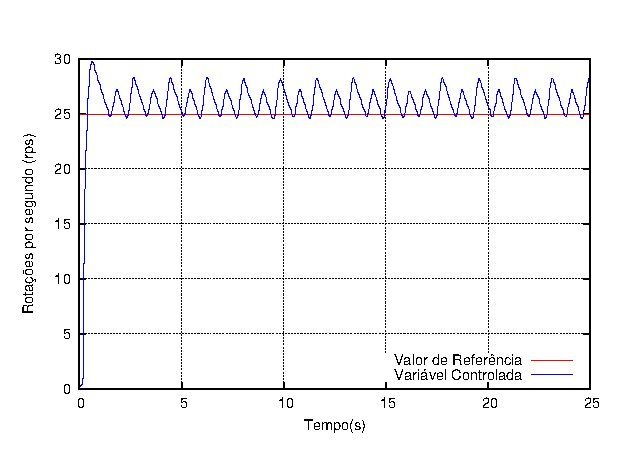
\includegraphics[scale=1]{./plot/acaoControle-ligaDesliga.eps}
\label{fig:AnexoAacaoControleLigaDesliga}

{\small Fonte: Próprio autor}
\end{figure}

A Figura \ref{fig:AnexoAacaoControleLigaDesliga} mostra o gráfico obtido no sistema de teste, onde a velocidade de rotação do motor oscila entre os valores de 25 e 30 rps, sendo o valor desejado em 25 rps. 
Todas estas oscilações podem representar perda de energia, pois o motor está recebendo energia em excesso sem necessidade, porém sua implementação é simples e não requer um conhecimento específico e aprofundado de controle.


%
%\begin{figure}[!htb]
%\centering
%\caption{Código da Ação de Controle Liga-Desliga}
%\begin{minipage}{0.8\linewidth}
%\begin{lstlisting}
%long controlador_LigaDesliga{ long setpoint, long sensor }
%{
%  if( sensor > setpoint }
%    return( 0 );
%  else
%    return( 100 );
%}
%\end{lstlisting}
%\end{minipage}
%\label{fig:codigoAcaoLigaDesliga}

%{\small Fonte: Próprio autor}
%\end{figure}

%O código fonte que gerou o resultado obtido na Figura \ref{fig:acaoControleLigaDesliga} é  mostrado na Figura \ref{fig:codigoAcaoLigaDesliga}, sendo apresentada apenas a função que realiza função de controle, que neste caso tem como parâmetros de entrada os valores de \textit{\texttt{setpoint}} e do \textit{\texttt{sensor}} e o seu valor de retorno é o parâmetro de entrada da função de acionamento da modulação por largura de pulso (\textit{PWM - Pulse Width Modulation}), que neste caso utiliza apenas os valores extremos.



\subsection{ Controlador Proporcional (P) } 

 No controle proporcional, 
o erro é multiplicado por uma constante \emph{kp} 
gerando o sinal \emph{u\{t\}}, 
que é a variável manipulada que atua sobre o 
sistema \emph{g(t)}.

\begin{equation}
 u(t) = kp . e(t)
\label{eq:acaoP}
\end{equation}


O diagrama de blocos da Figura \ref{fig:AnexoAmalhaFechadaP} mostra o bloco \emph{kp} que tem seu comportamento descrito pela Equação \ref{eq:acaoP} e que atua diretamente sobre o sistema através da variável manipulada $u(t)$.

\begin{figure}[!htb]
\centering
\caption{ Diagrama em blocos de sistema de controle em malha fechada utilizando notação matemática}
\begin{tikzpicture}[scale=0.6]
%\draw [lightgray](-3,0) grid (17, 2);
%\draw [lightgray](-3,0) grid (17,-3);
%\draw [semithick,red] (0,0) circle (0.1);

\draw (-3,1) -- (0,1);
\draw [fill]( 0,1) -- (-0.2, 1.1) -- ( -0.2,0.9) -- (0,1);
\draw [semithick,black] (1,1) circle (1.0); % Somador
\draw (2.0,1) -- (4,1);
\draw [fill]( 4,1) -- ( 3.8, 1.1) -- ( 3.8,0.9) -- ( 4,1);
\draw [black, thick](4,0) rectangle (7, 2) ; % Controlador 
\draw (7,1) -- (11,1);
\draw [fill]( 11,1) -- (10.8, 1.1) -- (10.8,0.9) -- (11,1);
\draw [black, thick](11,0) rectangle (14, 2) ; % Planta
\draw (14,1) -- (17,1);
\draw [fill](17,1) -- (16.8, 1.1) -- (16.8,0.9) -- (17,1);

\draw [black, thick](7.5,-1) rectangle (10.5, -3) ; % Sensor
\draw (14.4, 1) -- (14.4, -2) -- (10.5,-2);
\draw ( 7.5,-2) -- ( 1, -2) -- (1,0);
\draw [fill](1,0) -- (1.2,-0.2) -- (0.8,-0.2) -- (1,0);

\node [above] at (-1.5,1){r(t)};
\node at (0.4,1){+};
\node at (1,0.4){-};
\node [above] at (3.0,1){e(t)};
\node at ( 5.5, 1){kp};
\node [above] at (9.0,1){u(t)};
\node at (12.5, 1){g(t)};
\node [above] at (16.0,1){c(t)};
\node at ( 9.0,-2){h(t)};

\end{tikzpicture}
\label{fig:AnexoAmalhaFechadaP}

{\small Fonte: Próprio autor}
\end{figure}

Variando o valor de $kp$ pode-se ver pela Figura \ref{fig:AnexoAacaoP} que quanto maior o seu valor, mais rápida é a resposta do sistema, ou seja, menor é o tempo necessário para alcançar o valor de referência, porém, depois de um determinado valor, o sistema apresenta um sobressinal, que pode ou não ser tolerável, dependendo das exigências da aplicação.

\begin{figure}[!htb]
\centering
\caption{Ação de Controle Proporcional}
\center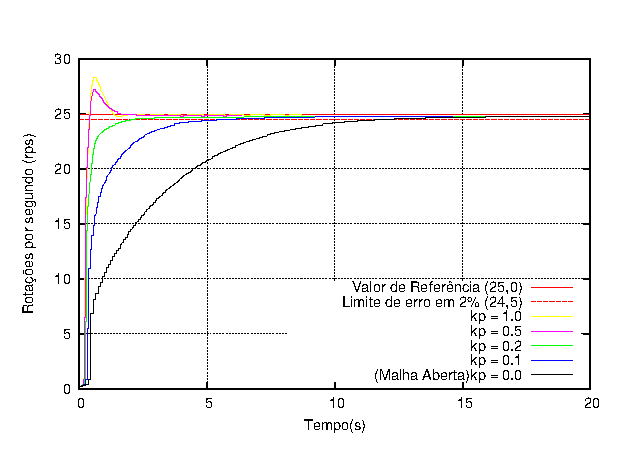
\includegraphics[scale=1.4]{./plot/acaoP.eps}
\label{fig:AnexoAacaoP}

{\small Fonte: Próprio autor}
\end{figure}

%O controlador que foi implementada a função proporcional está apresentado na Figura \ref{fig:codigoControladorP}, onde pode-se verificar a utilização de variáveis do tipo ponto flutuante (\emph{float}) para obtenção de maior precisão nos cálculos e consequantemente, no controle. O nome das variáveis faz alusão a sua representação no diagrama de blocos da Figura \ref{fig:malhaFechadaP}.

%A função implementada, declarada na linha 7 possui três parâmetros de entrada e possui um parâmetro de retorno, sendo:
%\begin{itemize}
%  \item $setpoint$ : recebe o valor de rotação desejado ao sistema, o valor de referência;
%  \item $max$ : representa o máximo valor que o sistema alcança;
%  \item $sensor$ : recebe o valor de rotação atual da planta;
%  \item $return $ : Parâmetro de retorno da função que assume um valor entre 0 e 100, pois é o parâmetro de entrada do controlador PWM que efetua o acionamento do motor.

%\end{itemize}



%\begin{figure}[!htb]
%\centering
%\caption{Código da Ação de Controle Proporcional}
%\begin{minipage}{0.8\linewidth}
%\lstset{firstnumber=1}
%\begin{lstlisting}
%float kp = 0.1;
%float ki = 0.0002;
%float kd = 2.0;
%float yT, rT, eT, iT, dT, uT;
%long  Cout, pwmAlvo;

%long controlador{ long setpoint, long max, long sensor }
%{
%    rT = (float) setpoint;
%    yT = (float) sensor;
%    pwmAlvo = ((setpoint*100)/max);

    
%    eT = rT - yT;
    
%    uT = kp*eT;

%    Cout = pwmAlvo + uT;

%    if( Cout < 0 )
%        Cout = 0;
%    else if( Cout >= 100 )
%        Cout = 100;

%    return( Cout );
%}
%\end{lstlisting}
%\end{minipage}
%\label{fig:codigoControladorP}

%{\small Fonte: Próprio autor}
%\end{figure}


%Nas linhas 9 e 10 os parâmetros de entradas são convertidos em ponto flutuante para realização dos cálculos e atribuidos às respectivas variáveis auxiliares.

%A variável \emph{pwmAlvo} recebe o valor percentual da velocidade de referência, como a velocidade mínima é zero, basta dividir o \emph{setpoint} pelo valor \emph{max} e multiplicar por \emph{100} conforme feito na linha 11.


%A linha 14 realiza o cálculo do erro, subtraindo do valor de referência (\emph{rT}) o valor do erro (\emph{ht}).

%Na linha 18 a variável manipilada recebe o erro (\emph{eT}) sendo multiplicado proporcionalmente pelo coeficiente kp, que caracteriza esta configuração de controle.

%A variável \emph{Cout}, é a variável com o valor que será o retorno da função, que serve de parâmetro de entrada ao gerador de sinal PWM que atua sobre o motor.

%\emph{Cout} recebe o valor da variável \emph{pwmAlvo} que é a aplicação de um degrau com valor de referência do sistema somado somada a \emph{uT} que possui o valor proporcional ao erro do sistema. 

%Inicialmente, considerando o sistema em repouso, o erro possui um valor alto, então, Cout é inicializada com um valor bem maior do que o necessário para gerar o valor de referência, ou seja, um valor de pwm referente a uma velocidade bem maior do que os \emph{25 rps} de referência da aquisição mostrada na Figura \ref{fig:acaoP}. Conforme o sistema começa a girar, e a velocidade aumenta, o erro diminui, o que diminui o incremento ao \emph{pwmAlvo}, até que este incremento seja zero quando o valor lido pelo sensor alcançar o valor de referência, que é o próprio valor do degrau que está em \emph{pwmAlvo}.

%O código entre as linhas 20 e 23 são necessárias apenas para não gerar um valor incorreto para o parâmetro do PWM, o que poderia causar falhas no acionamento. 








\subsection{ Controlador Integral (I) }

O controlador integral atua acumulando o erro do sistema, conforme equação descrita abaixo:


\begin{equation}
u(t) = ki \int_{0}^{\infty} e(t) dt
\end{equation}

A resposta apresentada pelo sistema está plotada na Figura \ref{fig:AnexoAacaoI} e mostra que ao aumentar o valor do coeficiente \emph{ki} o sistema começou a oscilar e demorou mais para estabilizar dentro de um valor limite próximo ao valor de referência. 

\begin{figure}[!h]
\centering
\caption{Ação de Controle Integral}
\center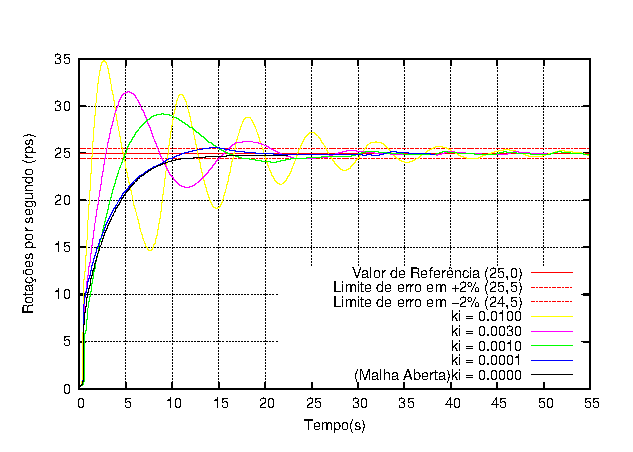
\includegraphics[scale=1.3]{./plot/acaoI.eps}
\label{fig:AnexoAacaoI}

{\small Fonte: Próprio autor}
\end{figure}

%A Figura \ref{fig:codigoControladorI} mostra o código da função que implementou o controlador com ação integral, responsáveis por gerar propriamente a ação de integração do erro.


%\begin{figure}[!htb]
%\centering
%\caption{Código da Ação de Controle Integral}
%\begin{minipage}{0.8\linewidth}
%\lstset{firstnumber=13}
%\begin{lstlisting}

%    eT = rT - yT;
%    iT += eT * i; 
%    uT = iT;
%\end{lstlisting}
%\end{minipage}
%\label{fig:codigoControladorI}

%{\small Fonte: Próprio autor}
%\end{figure}

A ação de integração é uma somatória de pequenas amostras do erro, que somadas ao longo do tempo levam o sistema a um erro zero, porém demoram mais tempo para alcançar a estabilidade e facilmente geram sobressinal.










\subsection{ Controlador Proporcional + Integral (PI) }

O controlador Proporcional Integral (PI) como o próprio nome indica, é a união das ações de controle que levam seu nome, e busca unir as suas propriedades.
 
\begin{equation}
u(t) = kp.e(t) + ki \int_{0}^{\infty} e(t) dt
\end{equation}


O intuito neste controlador é reduzir o tempo de resposta do sistema pelo controle proporcional e ao mesmo tempo gerar um erro nulo quando a estabilidade é atingida.





\begin{figure}[!htb]
\centering
\caption{ Diagrama em blocos de sistema de controle em malha fechada utilizando notação matemática}
\begin{tikzpicture}[scale=0.6]

%\draw [lightgray](-3,0) grid (18, 2);
%\draw [lightgray](-3,0) grid (18,-5);
%\draw [semithick,red] (0,0) circle (0.1);

\draw (-3,1) -- (0,1);
\draw [fill]( 0,1) -- (-0.2, 1.1) -- ( -0.2,0.9) -- (0,1);
\draw [semithick,black] (1,1) circle (1.0); % Somador
\draw (2.0,1) -- (4,1);
\draw [fill]( 4,1) -- ( 3.8, 1.1) -- ( 3.8,0.9) -- ( 4,1);
\draw [black, thick](4,0) rectangle (6, 2) ; % Controlador P 
\draw (6,1) -- (8,1);
\draw [fill]( 8,1) -- (7.8, 1.1) -- ( 7.8,0.9) -- (8,1);
\draw [semithick,black] (9,1) circle (1.0); % Somador 2
\draw (10.0,1) -- (12,1);
\draw [fill]( 12,1) -- (11.8, 1.1) -- (11.8,0.9) -- (12,1);
\draw [black, thick](12,0) rectangle (15, 2) ; % Planta
\draw (15,1) -- (18,1);
\draw [fill](18,1) -- (17.8, 1.1) -- (17.8,0.9) -- (18,1);

\draw (3,1) -- (3,-2) -- (4,-2);
\draw [fill](4,-2) -- (3.8, -2.1) -- (3.8,-1.9) -- (4,-2);
\draw [black, thick](4,-1) rectangle (6,-3) ; % Controlador I
\draw (6,-2) -- (9,-2) -- (9,0);
\draw [fill](9,0) -- (8.9, -0.2) -- (9.1,-0.2) -- (9,0);



\draw [black, thick](7.5,-3) rectangle (10.5, -5) ; % Sensor
\draw (16, 1) -- (16, -4) -- (10.5,-4);
\draw ( 7.5,-4) -- ( 1, -4) -- (1,0);
\draw [fill](1,0) -- (1.2,-0.2) -- (0.8,-0.2) -- (1,0);

\node [above] at (-1.5,1){r(t)};
\node at (0.4,1){+};
\node at (1,0.4){-};
\node [above] at (3.0,1){e(t)};
\node at ( 5.0, 1){kp};
\node at (5.0,-2) {ki};
\node at (8.4,1){+};
\node at (9,0.4){+};
\node [above] at (11.0,1){u(t)};
\node at (13.5, 1){g(t)};
\node [above] at (17.0,1){c(t)};
\node at ( 9.0,-4){h(t)};

\end{tikzpicture}
\label{fig:AnexoAmalhaFechadaPI}

{\small Fonte: Próprio autor}
\end{figure}

Variando o valor de $kp$ pode-se ver pela Figura \ref{fig:AnexoAacaoP} que quanto maior o seu valor, mais rápida é a resposta do sistema, ou seja, menor é o tempo necessário para alcançar o valor de referência, porém, depois de um determinado valor, o sistema apresenta um sobressinal, que pode ou não ser tolerável, dependendo das exigências da aplicação.

%\begin{figure}[!htb]
%\centering
%\caption{Ação de Controle Proporcional}
%\center\includegraphics[scale=1.4]{./imagens/acaoPI.eps}
%\label{fig:acaoP}

%{\small Fonte: Próprio autor}
%\end{figure}






\begin{figure}[!htb]
\caption{Ação de Controle Proporcional Integral}
\center\includegraphics[scale=1.2]{./plot/acaoPI.eps}
\label{fig:AnexoAacaoPI}

{\small Fonte: Próprio autor}
\end{figure}

Como pode-se ver no gráfico da Figura \ref{fig:AnexoAacaoPI} foi utilizado um valor de $ki = 0.1$ para obter uma subida em um tempo tido como bom, ou seja, subida mais rápida e sem gerar sobressinal, de acordo com os valores mostrados na Figura \ref{fig:AnexoAacaoP}.





%\begin{figure}[!htb]
%\centering
%\caption{Código da Ação de Controle Proporcional Integral}
%\begin{minipage}{0.8\linewidth}
%\lstset{firstnumber=13}
%\begin{lstlisting}

%    eT = rT - yT;
%    iT += eT * i; 
%    uT = iT + p*eT;
%\end{lstlisting}
%\end{minipage}
%\label{fig:codigoControladorPI}

%{\small Fonte: Próprio autor}
%\end{figure}

%O código da Figura \ref{fig:codigoControladorPI} mostra a implementação das funções de controle proporcional e integral, sendo que a linha 15 mostra a somatória característica do controle integral.










%\subsection{ Controlador Proporcional + Derivativo (PD) }

%A ação de controle proporcional e derivativo propicia uma resposta mais rápida, pois a ação derivativa gera um grande erro se houver variações abruptas.

%\begin{equation}
%u(t) = kp.e(t) + kd. \frac{d e(t)}{dt}
%\end{equation}

%A figura \ref{fig:acaoPD} mostra que a resposta do sistema é a mais rápida dos ações de controle estudadas, e também gera o maior sobressinal. 


%\begin{figure}[!htb]
%\centering
%\caption{Ação de Controle Proporcional Derivativo}
%\center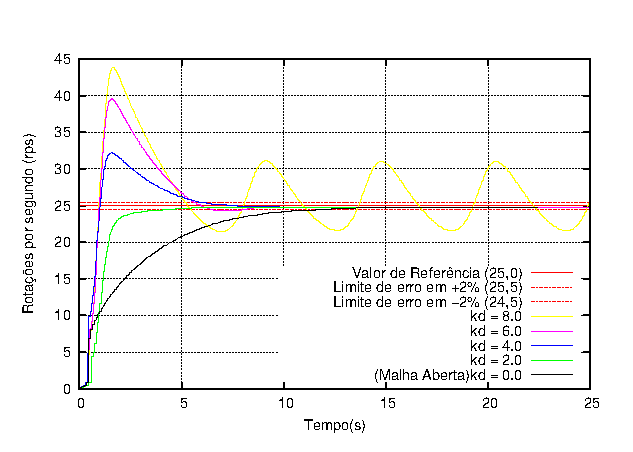
\includegraphics[scale=1.1]{./imagens/acaoPD.eps}
%\label{fig:acaoPD}

%{\small Fonte: Próprio autor}
%\end{figure}

% A linha 13 da Figura \ref{fig:codigoControladorPD} mostra como foi codificada a ação de controle Derivativa modificada.

%\begin{figure}[!htb]
%\centering
%\caption{Código da Ação de Controle Proporcional Derivativo}
%\begin{minipage}{0.8\linewidth}
%\lstset{firstnumber=13}
%\begin{lstlisting}
%    dT = (eT - (rT-yT)) * d;
%    eT = rT - yT;
%
%    uT = dT + p*eT;
%\end{lstlisting}
%\end{minipage}
%\label{fig:codigoControladorPD}

%{\small Fonte: Próprio autor}
%\end{figure}

%A ação de controle derivativa (PD) é modificada pois é utilizada a diferença do erro na iteração anterior com o erro com os dados atuais, diferente do que ocorre com o controlador PD teórico, onde a derivada implica na diferença entre o valor atual e uma pequena variação positiva do tempo, ou seja, uma amostra futura, que é impossível de ser obtida na pratica. 










%\subsection{ Controlador Proporcional + Integral + Derivativo (PID) }

%O controlador Proporcional Integral Derivativo é uma das configurações mais utilizadas por sua versatilidade, unindo as características que permitem ajustar o tempo de subida, o sobressinal e o erro de estado estacionário, conforme a necessidade e a aplicação.

%\begin{equation}
%u(t) = kp.e(t) + ki \int_{0}^{\infty} e(t) dt + kd. \frac{d e(t)}{dt}
%\end{equation}

%O controlador PID pode ser implementado de diversas formas, pode ter o parâmetro proporcional influenciando diretamente as demais ações, ou não, como neste caso onde as ações de controle são utilizadas de forma independentes, e o erro é utilizado para cada uma das partes da soma do sinal da variável manipulada ($u(t)$).

%\begin{figure}[!htb]
%\centering
%\caption{Ação de Controle Proporcional Integral Derivativo}
%\center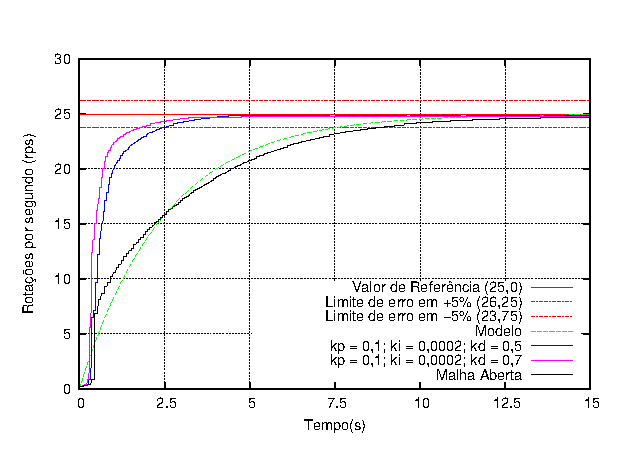
\includegraphics[scale=1.4]{./imagens/acaoPID.eps}
%\label{fig:acaoPID}

%{\small Fonte: Próprio autor}
%\end{figure}

%Os dois sinais utilizando o controle PID utilizou parâmetros já testados nos controladores anteriores para obter um resultado desejado, onde o sistema responde de forma bem rápida ao estímulo de entrada, tendo um tempo de subida entre 3 e 4 segundos para atingir a estabilidade com erro de estado estacionário menor do que 2\%, sem gerar sobressinal.


%Em comparação ao sinal de controle em malha aberta, que a estabilidade é alcançada em um tempo de aproximadamente 12 segundos, o ganho de velocidade é consideravel para o sistema estudado, pois foi reduzido a pelo menos um terço do tempo original.

%A Figura \ref{fig:codigoControladorPID} mostra a codificação completa dos parâmetros do PID, onde pode-se perceber que sua implementação é simples, apesar da teoria ser complexa. 

%\begin{figure}[!htb]
%\centering
%\caption{Código da Ação de Controle Proporcional Integral Derivativo}
%\begin{minipage}{0.8\linewidth}
%\lstset{firstnumber=13}
%\begin{lstlisting}
%    dT = (eT - (rT-yT)) * d;
%    eT = rT - yT;
%    iT += eT * i; 
%    uT = p*eT + iT + dT;
%\end{lstlisting}
%\end{minipage}
%\label{fig:codigoControladorPID}

%{\small Fonte: Próprio autor}
%\end{figure}


%Para o microcontrolador efetuar as subtrações é algo que requer pouco processamento, mas as multiplicações são bem mais complexas e exigem mais memória e tempo de processamento, e é claro que trabalhando em ponto flutuante esta complexidade também é muito grande. O controlador utilizado possui uma unidade de processamento de ponto flutuante, o que possibilitou uma performance capaz de efetuar todos os cálculos sem afetar a leitura de velocidade do sistema.

%%%%%%%%%%%%%%%%%%%%%%%%%%%%%%%%%%%%%%%%%%%%%%%%%%%%%%%%%%%
%\section{Requisitos de desempenho do sistema}
%%%%%%%%%%%%%%%%%%%%%%%%%%%%%%%%%%%%%%%%%%%%%%%%%%%%%%%%%%%

%Os sistemas de controle buscam atender os chamados requisitos de desempenho do sistema, que de um modo geral se efetuam através de modificações das características da relação entrada/saída para se obter os valores desejados dessa relação, ou ainda ajustar o comportamento da saída para uma dada entrada específica.

%Os principais e mais comuns requisitos de desempenho dos sistemas são associados a velocidade de resposta, presença ou não de oscilações e a exatidão da resposta do sistema em relação ao valor desejado, chamada de erro de regime estacionário.

%O erro de regime estacionário, mostrada na Figura \ref{fig:funcaoResposta}, é uma medida que vai tender a zero em sistemas ideais, mas que na realidade não alcança o valor zero, assim assume-se um valor aceitável, 5\% do valor da resposta desejada para sistemas não críticos e 2\% para sistemas de maior grau de criticidade, para assumir que o sistema entrou em estabilidade, e a resposta real é aceita como tendo atingido o valor de resposta desejada. 

%\begin{figure}[!htb]
%\centering
%\caption{Gráfico da função Resposta}
%\center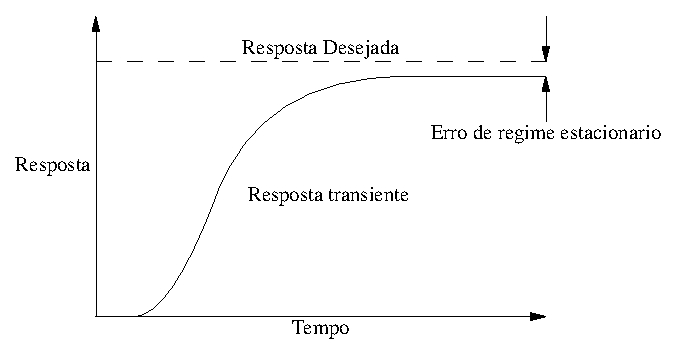
\includegraphics[scale=1]{./imagens/C400grafico.eps}
%\label{fig:funcaoResposta}

%{\small Fonte: Próprio autor}
%\end{figure}

%Para realizar o controle de um sistema é necessário que estejam bem definidos os seus requisitos, que são os objetivos a serem atendidos. Quando um sistema por si só já atende aos requisitos, não há a necessidade de controle. De forma oposta, é projetado o sistema de controle, que pode ser em malha aberta ou fechada, clássico ou moderno dependendo das características físicas do sistema. 

%Para a execução de um sistema de controle podem ser verificados requisitos do sistema de duas formas básicas, sendo a primeira através dos testes e levantamento empírico da sua curva de resposta ou através de seu modelo matemático, quando trabalha-se com elementos já bem estudados e com a equação que representa seu comportamento empírico bem estabelecida por diversos estudos anteriores.



%\newpage






\chapter[Apêndice B: Modelo matemático do processo]{Apêndice B: \\ Modelo matemático do processo}
\newpage
%\section*{ Obtenção de um modelo do processo }
Para melhor compreensão dos modelos dinâmicos dos sistemas, é utilizado o Diagrama de blocos do comportamento do sistema em malha aberta, conforme Figura \ref{fig:AnexoBmalhaAberta}\cite{Ogata}.


%\begin{comment}


\begin{figure}[!htb]
\centering
\caption{ Diagrama de blocos de sistema de controle em malha aberta}
\begin{tikzpicture}[scale=0.85]
%\draw [lightgray](0,0) grid (15,2);
\draw (0,1) -- (3,1);
\draw [black, thick](3,0) rectangle (6, 2) ; 
\draw (6,1) -- (9,1);
\draw [black, thick](9,0) rectangle (12, 2) ; 
\draw (12,1) -- (15,1);

\draw [fill]( 3,1) -- ( 2.8, 1.1) -- ( 2.8,0.9) -- ( 3,1);
\draw [fill]( 9,1) -- ( 8.8, 1.1) -- ( 8.8,0.9) -- ( 9,1);
\draw [fill](15,1) -- (14.8, 1.1) -- (14.8,0.9) -- (15,1);

\node at ( 4.5, 1){Controlador};
\node at (10.5, 1){Planta};
\node [above] at ( 1.5,1){Valor de};
\node [below] at ( 1.5,1){Referência};
\node [above] at ( 7.5,1){Variável};
\node [below] at ( 7.5,1){Manipulada};
\node [above] at (13.5,1){Variável};
\node [below] at (13.5,1){Controlada};
\end{tikzpicture}
\label{fig:AnexoBmalhaAberta}

{\small Fonte: \cite{Ogata}}
\end{figure}

%\end{comment}

Utilizando variáveis para cada elemento do Diagrama de blocos,
conforme Figura \ref{fig:AnexoBAcaoMalhaAberta},
de forma a representá-los nas equações, temos então que:



\begin{figure}[!htb]
\centering
\caption{ Sistema de controle em malha aberta}
\begin{tikzpicture}[scale=0.85]
%\draw [lightgray](0,0) grid (15,2);
\draw (0,1) -- (3,1);
\draw [black, thick](3,0) rectangle (6, 2) ; 
\draw (6,1) -- (9,1);
\draw [black, thick](9,0) rectangle (12, 2) ; 
\draw (12,1) -- (15,1);

\draw [fill]( 3,1) -- ( 2.8, 1.1) -- ( 2.8,0.9) -- ( 3,1);
\draw [fill]( 9,1) -- ( 8.8, 1.1) -- ( 8.8,0.9) -- ( 9,1);
\draw [fill](15,1) -- (14.8, 1.1) -- (14.8,0.9) -- (15,1);

\node at ( 4.5, 1.4){Controlador};
\node at ( 4.5, 0.6){f(t)};
\node at (10.5, 1.4){Planta};
\node at (10.5, 0.6){g(t)};
\node [above] at ( 1.5,1){r(t)};
\node [above] at ( 7.5,1){u(t)};
\node [above] at (13.5,1){c(t)};
\end{tikzpicture}
\label{fig:AnexoBAcaoMalhaAberta}

{\small Fonte: Próprio autor}
\end{figure}


Onde: 

%\begin{itemize}
%\item 
\hspace{1cm} $r(t)$: Valor de Referência em rotações por segundo [rps];

%\item 
$\hspace{1cm} f(t)$: Controlador que converte rps em \% PWM para acionar o motor;

%\item 
$\hspace{1cm} u(t)$: Variável Manipulada é o valor percentual do PWM;

%\item 
$\hspace{1cm} g(t)$: Planta ou Processo formado pelo motor DC com o disco acoplado no eixo;

%\item 
$\hspace{1cm}  c(t)$: Variável Controlada é a velocidade de rotação do eixo em rps.

%\end{itemize}



O sistema físico aqui estudado possui comportamento exponencial que pode ser descrito pela equação \ref{eq:ftSistOrdem1}. 






\begin{equation}
	 \frac{d c(t)}{dt} + c(t) = r(t) \rightarrow  \mathscr{L} \to \frac{C(s)}{R(s)} = \frac{K}{s + a} 
\label{eq:ftSistOrdem1}
\end{equation}

Onde:

\setlength{\parindent}{2cm}

$t$ : tempo,$ r(t) = 0$ , para t $<$ 0;

$\mathscr{L}$ : Operador de Laplace;

$c(t)$ : Variável controlada no domínio do tempo;

$C(s)$ : Variável controlada no domínio da frequência;

$r(t)$ : Valor de referência (\emph{setpoint}) no domínio do tempo;

$R(s)$ : Valor de referência (\emph{setpoint}) no domínio da frequência.

$K$ : Constante de proporcionalidade;

$s$ : Variável complexa de Laplace;

$a$ : Polo da função.
\setlength{\parindent}{1cm}



Sendo assim, para um estímulo de entrada do tipo \textbf{degrau}, com amplitude \textbf{A}, temos $ R(s) = \frac{A}{s}$ e aplicando a Transformada Inversa de Laplace:

\begin{equation}
C(s) = \frac{K}{s+a} \frac{A}{s} \rightarrow \mathscr{L}^{-1} \to c(t) = \frac{K A}{a} (1 - e^{-at})
\label{eq:degrauA}
\end{equation}

A Figura \ref{fig:AnexoBacaoMalhaAberTau} mostra um sinal do tipo degrau com amplitude \textbf{A} aplicado ao sistema de teste, que responde conforme um sistema de primeira ordem como mostrado na Figura \ref{fig:AnexoBcRegime}. 


%A partir de um determinado instante de tempo, entra em regime constante ($c_{reg}$), alcançando o valor de referência dado pelo degrau de amplitude A. Assim quando $ t \rightarrow \infty $  então $ c_{reg} \rightarrow A $:




\begin{figure}[!htb]
\centering
\caption{Sistema de Primeira Ordem}
\subfloat[Sinal de entrada tipo degrau com amplitude A]{\label{fig:AnexoBdegrauA}
\begin{tikzpicture}[scale=0.75]
\draw [lightgray, dashed](0,0) grid (8.8,5.8);
\draw [->] (0,0) -- (9,0);
\draw [fill] (0,6.2) -- (-0.1, 5.8) -- (0.1,5.8) -- (0,6.2);
\draw [->] (0,0) -- (0,6);
\draw [fill] (9.2,0) -- (8.8,0.1) -- (8.8,-0.1)--(9.2,0.0);
\node at (9.0,-0.5) {$t$};
\node at (0.2,6.5) {$r(t)$};
\draw [red, ultra thick] (0.0,5.0) -- (9.0,5.0);
\draw [red, ultra thick] (0.0,0.0) -- (0.0,5.0);
\node at (-0.5,5.0)[red]{$A$};
\end{tikzpicture} }
\subfloat[Resposta transitória e regime de acomodação]{\label{fig:AnexoBcRegime}
\begin{tikzpicture}[scale=0.75]
\draw [lightgray, dashed](0,0) grid (8.8,5.8);
\draw [->] (0,0) -- (9,0);
\draw [fill] (0,6.2) -- (-0.1, 5.8) -- (0.1,5.8) -- (0,6.2);
\draw [->] (0,0) -- (0,6);
\draw [fill] (9.2,0) -- (8.8,0.1) -- (8.8,-0.1)--(9.2,0.0);
\node at (9.0,-0.5) {$t$};
\node at (0.2,6.5) {$c(t)$};
\node at (-0.5,5.0)[blue]{$C_{reg}$};
\draw [blue, ultra thick] (0,0) to [out=85, in=180] (6,5);
\draw [blue, ultra thick] (6,5) -- (9,5);
\end{tikzpicture}}
\label{fig:AnexoBsistPrimeiraOrdem}

{\small Fonte: Próprio autor}
\end{figure}

%\begin{equation}
%c_{reg} = \lim_{t \rightarrow \infty} \frac{KA}{a}(1-e^{-at}) = \frac{KA}{a}
%\label{eq:cregime}
%\end{equation}



%Aplicando o Teorema do Valor Final pode-se ver que o \emph{$c_{reg}$} estabiliza em um valor constante como mostrado pela Equação \ref{eq:teoremaValorFinal}:

%\begin{equation}
%C_{reg} = \lim_{s \rightarrow 0} sC(s) = \lim_{s \rightarrow 0} s\ \frac{K}{s+a}\frac{A}{s} = \frac{KA}{a}
%\label{eq:teoremaValorFinal}
%\end{equation}



Matematicamente, quanto maior o valor de \emph{t} na Equação \ref{eq:degrauA}, o resultado da exponenencial tende a zero, levando a um resultado que depende apenas das constantes para o valor de referência. 

Tomando $t= \frac{1}{a} = a^{-1} = \tau$ para gerar um valor conhecido em $e^{-at}$, da Equação \ref{eq:degrauA} temos:


\begin{equation}
c(a^-1) = \frac{KA}{a}(1-e^{-(a.a^{-1})}) = \frac{KA}{a}(1-e^{-1}) = \frac{KA}{a}.0,63 = 0,63 . C_{reg}
\end{equation}

A Figura \ref{fig:AnexoBconstTempo} mostra a constante de tempo $\tau$, que é atingida quando o sistema alcança 63\% do seu valor de regime. Como sabemos que $\tau = \frac{1}{a}$, então o polo do sistema, que leva o denominador da Equação \ref{eq:degrauA} a zero, é:

\begin{equation}
a = \frac{1}{\tau}
\end{equation}



\begin{figure}
\centering
\caption{Constante de tempo}
\begin{tikzpicture}[scale=1.0]
\draw [lightgray, dashed](0,0) grid (8.8,5.8);

\draw [->] (0,0) -- (9,0);
\draw [fill] (0,6.2) -- (-0.1, 5.8) -- (0.1,5.8) -- (0,6.2);
\draw [->] (0,0) -- (0,6);
\draw [fill] (9.2,0) -- (8.8,0.1) -- (8.8,-0.1)--(9.2,0.0);

\node at (9.0,-0.5) {$t$};
\node at (0.2,6.5) {$c(t)$};

\node at (-0.5,5.0)[blue]{$C_{reg}$};
\node at (-1,5.0*0.63)[purple]{$0,63.c_{reg}$};
\draw [purple, ultra thick, dashed] (0.0,5.0*0.63) -- (1.45,5.0*0.63)
						   -- (1.45,0.0);
\draw [blue, ultra thick] (0,0) to [out=85, in=180] (6,5);
\draw [blue, ultra thick] (6,5) -- (9,5);

\draw [<->] (0.0,-0.4) -- (1.45,-0.4); 
\node at (1.45/2,-0.7){$\tau$};

\end{tikzpicture}
\label{fig:AnexoBconstTempo}

{\small Fonte: Próprio autor}
\end{figure}

Portanto:

\begin{equation}
K = \frac{ac_{reg}}{A}
\label{eq:calcK}
\end{equation}

%\begin{tikzpicture}
%\begin{axis}
%\addplot[title=Gráfico de uma função, 
%	xlabel = {$x$}, ylabel={$y$},
% 	red!70!blue, very thick, samples=200,
%	domain=-3:3]{x/(x^4-3*x^2+4)};
%\end{axis}
%\end{tikzpicture}



%\begin{figure}[!htb]
%\center	
%\includegraphics[scale=1.2]{./imagens/ftMalhaAberta.eps} 
%\label{fig:ftMalhaAberta} 
%\caption{ Função de Transferência empírica da planta}
%\end{figure}





A Figura \ref{fig:AnexoBacaoMalhaAberTau} mostra um sinal do tipo
degrau aplicado como referência no valor de \emph{25 rps}, a curva de
comportamento real medida empiricamente e a curva aproximada calculada
pelo método determinístico como segue, e ainda possui uma linha
indicativa que mostra o ponto de intercepção da curva ao valor de 63\%
do valor de referência, e foi gerado um gráfico com
divisões no eixo do Tempo no valor de $\tau = 2,5s $.

\begin{figure}[!htb]
\caption{Ação de Controle em Malha Aberta}
\center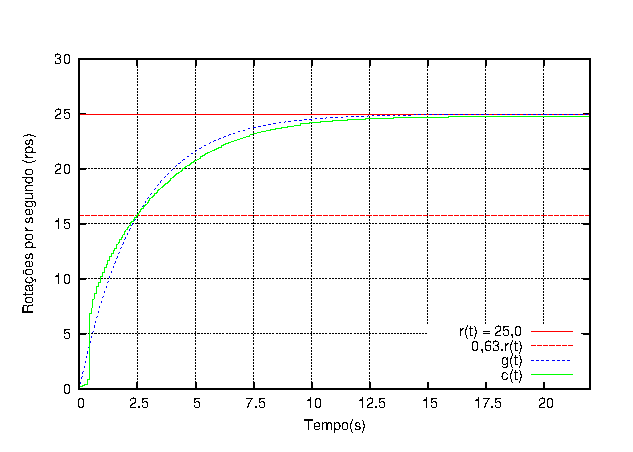
\includegraphics[scale=1.4]{./plot/acaoMalhaAbertaTau.eps}
\label{fig:AnexoBacaoMalhaAberTau}

{\small Fonte: Próprio autor}
\end{figure}


Calculando o polo da função:
\begin{equation}
  a = \frac{1}{\tau} = \frac{1}{2,5} = 0,4
\end{equation}

Como $c_{reg} = 25$ e $A$ também é $25$ então na Equação \ref{eq:calcK} $K = a$ e assim temos que:

\begin{equation}
c(t) = \frac{KA}{a}(1-e^{-at}) = \frac{0,4.25}{0,4}(1-e^{-0,4.t}) = 25(1-e^{-0.4.t})
\end{equation}


Aplicando a Transformada de Laplace:

\begin{equation}
  \frac{C(s)}{R(s)} = \frac{K}{s+a} = \frac{0,4}{s+0,4}
\end{equation}


Para a equação no formato canônico tanto o numerador quanto o denominador são divididos pelo próprio valor de $K$. Assim temos que:

\begin{equation}
  \frac{C(s)}{R(s)} = \frac{1}{\tau s+1} = \frac{1}{2,5 s+1}
\end{equation}


Baseado no gráfico mostrado na Figura \ref{fig:AnexoBacaoMalhaAberTau}, o valor de tempo em que o motor assume a velocidade de referência é aproximadamente $5\tau$, 12,5 s, e como objetivo para uma primeira versão da implementação do controle utilizando LPA$E\tau$ é proposto que o sistema reduza o tempo de alcance da velocidade alvo em um tempo de no máximo $1\tau$, ou seja, $2,5 s$.






\end{document}





% bibliographystyle tipos
%http://www.cs.stir.ac.uk/~kjt/software/latex/showbst.html

%%%% Estrutura base do arquivo
%%[] http://www.demat.ufma.br/monografia.php <acesso em 12/10/2015>
%%%% Inclusão de pacote de acentuação Francês/Portugues
%%[] https://www.overleaf.com/help/61-how-do-i-do-to-use-letters-with-accents-e-dot-g-in-french-or-portuguese#.Vhwirc8Tr18 <acesso em 12/10/2015 


%http://link.periodicos.capes.gov.br/sfxlcl41?frbrVersion=2&ctx_ver=Z39.88-2004&ctx_enc=info:ofi/enc:UTF-8&ctx_tim=2015-10-27T23%3A55%3A45IST&url_ver=Z39.88-2004&url_ctx_fmt=infofi/fmt:kev:mtx:ctx&rfr_id=info:sid/primo.exlibrisgroup.com:primo3-Article-doaj&rft_val_fmt=info:ofi/fmt:kev:mtx:journal&rft.genre=article&rft.atitle=Implementation+of+PID+and+Fuzzy+PID+controllers+for+Temperature+control+in+CSTR&rft.jtitle=International+Journal+of+Advanced+Research+in+Computer+Science&rft.btitle=&rft.aulast=&rft.auinit=&rft.auinit1=&rft.auinitm=&rft.ausuffix=&rft.au=S.+Srinivasulu+Raju&rft.aucorp=&rft.date=20130501&rft.volume=04&rft.issue=05&rft.part=&rft.quarter=&rft.ssn=&rft.spage=12&rft.epage=&rft.pages=&rft.artnum=&rft.issn=0976-5697&rft.eissn=&rft.isbn=&rft.sici=&rft.coden=&rft_id=info:doi/&rft.object_id=&svc_val_fmt=info:ofi/fmt:kev:mtx:sch_svc&rft.eisbn=&rft_dat=%3Cdoaj%3E01c00f89709d40549e219bbc941a6a0a%3C/doaj%3E%3Cgrp_id%3E7778711627802309381%3C/grp_id%3E%3Coa%3E%3C/oa%3E&rft_id=info:oai/&svc.fulltext=yes&req.language=por

% http://link.periodicos.capes.gov.br/sfxlcl41?frbrVersion=3&ctx_ver=Z39.88-2004&ctx_enc=info:ofi/enc:UTF-8&ctx_tim=2015-10-27T23%3A55%3A45IST&url_ver=Z39.88-2004&url_ctx_fmt=infofi/fmt:kev:mtx:ctx&rfr_id=info:sid/primo.exlibrisgroup.com:primo3-Article-springer_jour&rft_val_fmt=info:ofi/fmt:kev:mtx:&rft.genre=&rft.atitle=Adaptive+fuzzy+tuning+of+PID+controllers&rft.jtitle=Neural+Computing+and+Applications&rft.btitle=&rft.aulast=Esfandyari&rft.auinit=&rft.auinit1=&rft.auinitm=&rft.ausuffix=&rft.au=Esfandyari%2C+Morteza&rft.aucorp=&rft.date=201312&rft.volume=23&rft.issue=1&rft.part=&rft.quarter=&rft.ssn=&rft.spage=19&rft.epage=28&rft.pages=&rft.artnum=&rft.issn=0941-0643&rft.eissn=1433-3058&rft.isbn=&rft.sici=&rft.coden=&rft_id=info:doi/10.1007%2Fs00521-012-1215-8&rft.object_id=&svc_val_fmt=info:ofi/fmt:kev:mtx:sch_svc&rft.eisbn=&rft_dat=%3Cspringer_jour%3E10.1007%2Fs00521-012-1215-8%3C/springer_jour%3E%3Cgrp_id%3E6653138538760267648%3C/grp_id%3E%3Coa%3E%3C/oa%3E&rft_id=info:oai/&svc.fulltext=yes&req.language=por

%http://link.periodicos.capes.gov.br/sfxlcl41?frbrVersion=2&ctx_ver=Z39.88-2004&ctx_enc=info:ofi/enc:UTF-8&ctx_tim=2015-10-27T23%3A55%3A45IST&url_ver=Z39.88-2004&url_ctx_fmt=infofi/fmt:kev:mtx:ctx&rfr_id=info:sid/primo.exlibrisgroup.com:primo3-Article-sciversesciencedirect_elsevier&rft_val_fmt=info:ofi/fmt:kev:mtx:&rft.genre=article&rft.atitle=A+multivariable+predictive+fuzzy+PID+control+system&rft.jtitle=Applied+Soft+Computing+Journal&rft.btitle=&rft.aulast=Savran&rft.auinit=&rft.auinit1=&rft.auinitm=&rft.ausuffix=&rft.au=Savran%2C+Aydogan&rft.aucorp=&rft.date=2012&rft.volume=&rft.issue=&rft.part=&rft.quarter=&rft.ssn=&rft.spage=&rft.epage=&rft.pages=&rft.artnum=&rft.issn=1568-4946&rft.eissn=&rft.isbn=&rft.sici=&rft.coden=&rft_id=info:doi/10.1016%2Fj.asoc.2012.11.021&rft.object_id=&svc_val_fmt=info:ofi/fmt:kev:mtx:sch_svc&rft.eisbn=&rft_dat=%3Csciversesciencedirect_elsevier%3ES1568-4946%2812%2900505-4%3C/sciversesciencedirect_elsevier%3E%3Cgrp_id%3E824269217450252803%3C/grp_id%3E%3Coa%3E%3C/oa%3E&rft_id=info:oai/&svc.fulltext=yes&req.language=por

%http://link.periodicos.capes.gov.br/sfxlcl41?frbrVersion=3&ctx_ver=Z39.88-2004&ctx_enc=info:ofi/enc:UTF-8&ctx_tim=2015-10-27T23%3A55%3A45IST&url_ver=Z39.88-2004&url_ctx_fmt=infofi/fmt:kev:mtx:ctx&rfr_id=info:sid/primo.exlibrisgroup.com:primo3-Article-gale_ofa&rft_val_fmt=info:ofi/fmt:kev:mtx:&rft.genre=article&rft.atitle=A+multivariable+predictive+fuzzy+PID+control+system.&rft.jtitle=Applied+Soft+Computing+Journal&rft.btitle=&rft.aulast=&rft.auinit=&rft.auinit1=&rft.auinitm=&rft.ausuffix=&rft.au=Savran%2C+Aydogan&rft.aucorp=&rft.date=20130501&rft.volume=13&rft.issue=5&rft.part=&rft.quarter=&rft.ssn=&rft.spage=2658&rft.epage=&rft.pages=&rft.artnum=&rft.issn=1568-4946&rft.eissn=&rft.isbn=&rft.sici=&rft.coden=&rft_id=info:doi/&rft.object_id=&svc_val_fmt=info:ofi/fmt:kev:mtx:sch_svc&rft.eisbn=&rft_dat=%3Cgale_ofa%3E339267889%3C/gale_ofa%3E%3Cgrp_id%3E8626435848081561867%3C/grp_id%3E%3Coa%3E%3C/oa%3E&rft_id=info:oai/&svc.fulltext=yes&req.language=por

%http://link.periodicos.capes.gov.br/sfxlcl41?frbrVersion=4&ctx_ver=Z39.88-2004&ctx_enc=info:ofi/enc:UTF-8&ctx_tim=2015-10-27T23%3A57%3A23IST&url_ver=Z39.88-2004&url_ctx_fmt=infofi/fmt:kev:mtx:ctx&rfr_id=info:sid/primo.exlibrisgroup.com:primo3-Article-springer_jour&rft_val_fmt=info:ofi/fmt:kev:mtx:&rft.genre=article&rft.atitle=Neuro+PID+control+of+power+generation+using+a+low+temperature+gap&rft.jtitle=Artificial+Life+and+Robotics&rft.btitle=&rft.aulast=Han&rft.auinit=&rft.auinit1=&rft.auinitm=&rft.ausuffix=&rft.au=Han%2C+Kun-Young&rft.aucorp=&rft.date=201109&rft.volume=16&rft.issue=2&rft.part=&rft.quarter=&rft.ssn=&rft.spage=178&rft.epage=184&rft.pages=&rft.artnum=&rft.issn=1433-5298&rft.eissn=1614-7456&rft.isbn=&rft.sici=&rft.coden=&rft_id=info:doi/10.1007%2Fs10015-011-0913-0&rft.object_id=&svc_val_fmt=info:ofi/fmt:kev:mtx:sch_svc&rft.eisbn=&rft_dat=%3Cspringer_jour%3E10.1007%2Fs10015-011-0913-0%3C/springer_jour%3E%3Cgrp_id%3E5844933895106062701%3C/grp_id%3E%3Coa%3E%3C/oa%3E&rft_id=info:oai/&svc.fulltext=yes&req.language=por



